\chapter{Linear Systems of Differential Equations}

\noindent
IN THIS CHAPTER we consider
  systems of differential equations
involving more than one unknown function. Such systems
arise in many physical applications.

\medskip\noindent
SECTION~10.1 presents examples of physical situations
that lead to systems of differential equations.

\medskip\noindent
 SECTION~10.2  discusses
linear systems of differential equations.

\medskip\noindent
SECTION~10.3 deals with the basic theory of homogeneous
linear systems.

\medskip\noindent
SECTIONS~10.4, 10.5, AND 10.6
present the theory of constant coefficient homogeneous systems.

\medskip\noindent
SECTION~10.7 presents the method of variation of parameters
for nonhomogeneous linear systems.

\vspace*{4in}


\newpage

\section{Introduction to Systems of Differential Equations}

\noindent
Many physical situations are modelled by systems of $n$ differential equations in $n$ unknown
functions, where $n\ge2$. The next three examples illustrate physical problems that lead to systems
of differential equations. In these examples and throughout this chapter we'll denote the
independent variable by $t$.

\begin{example}
  \label{example:10.1.1} \rm Tanks $T_{1}$ and $T_{2}$ contain 100 gallons and 300 gallons of salt
  solutions, respectively. Salt solutions are simultaneously added to both tanks from external
  sources, pumped from each tank to the other, and drained from both tanks
  (Figure~\ref{figure:10.1.1}). A solution with $1$ pound of salt per gallon is pumped into $T_{1}$
  from an external source at $5$~gal/min, and a solution with $2$ pounds of salt per gallon is
  pumped into $T_{2}$ from an external source at $4$~gal/min. The solution from $T_{1}$ is pumped
  into $T_{2}$ at 2 gal/min, and the solution from $T_{2}$ is pumped into $T_{1}$ at $3$ gal/min.
  $T_{1}$ is drained at $6$~gal/min and $T_{2}$ is drained at 3~gal/min. Let $Q_{1}(t)$ and
  $Q_{2}(t)$ be the number of pounds of salt in $T_{1}$ and $T_{2}$, respectively, at time $t>0$.
  Derive a system of differential equations for $Q_{1}$ and $Q_{2}$. Assume that both mixtures are
  well stirred.
\end{example}

\begin{figure}[H]
  \centering
  \color{blue}
  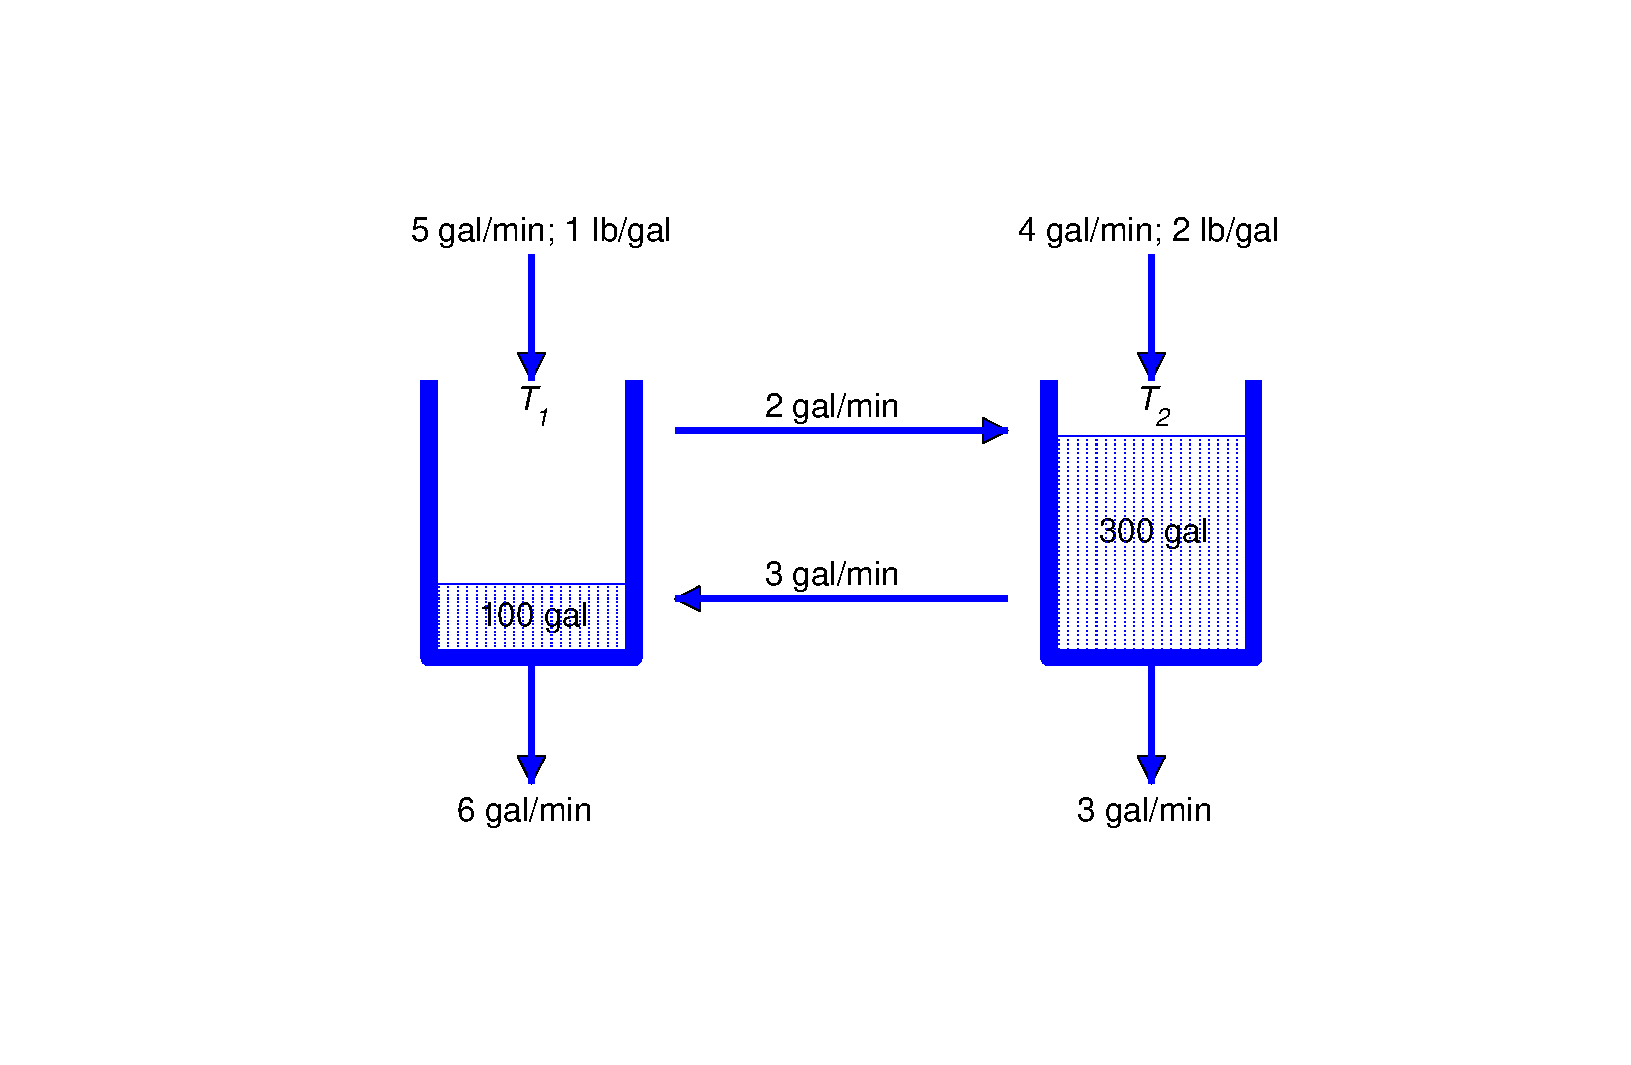
\includegraphics[bb=-78 148 689 643, width=5.67in, height=3.66in, keepaspectratio]{fig100101}
  \caption{}
  \label{figure:10.1.1}
\end{figure}

\solution As in Section~4.2, let {\color{blue}\it rate in\/} and {\color{blue}\it rate out\/} denote
the rates (lb/min) at which salt enters and leaves a tank; thus,
\begin{eqnarray*}
  Q_{1}' & = & (\mbox{rate in})_{1}-(\mbox{rate out})_{1}, \\[2\jot]
  Q_{2}' & = & (\mbox{rate in})_{2}-(\mbox{rate out})_{2}.
\end{eqnarray*}
Note that the volumes of the solutions in $T_{1}$ and $T_{2}$ remain constant at 100~gallons and
300~gallons, respectively.

$T_{1}$ receives salt from the external source at the rate of
\[
  \mbox{(1 lb/gal) }\times\mbox{ (5~gal/min)}=\mbox{ 5 lb/min},
\]
and from $T_{2}$ at the rate of
\[
  \mbox{(lb/gal in }T_{2})\times\mbox{ (3~gal/min) }=\frac{1}{300}Q_{2}\times3\\[2\jot]=\frac{1}{100}Q_{2}\mbox{ lb/min}.
\]
Therefore
\begin{equation}
  \label{eq:10.1.1}\mbox{(rate in)}_{1}=5+\frac{1}{100}Q_{2}.
\end{equation}
Solution leaves $T_{1}$ at the rate of 8~gal/min, since 6~gal/min are drained and 2~gal/min are
pumped to $T_{2}$; hence,
\begin{equation}
  \label{eq:10.1.2}(\mbox{rate out})_{1}=(\mbox{ lb/gal in T}_{1})\times\mbox{(8~gal/min) }=\frac{1}{100}Q_{1}\times8=\frac{2}{25}Q_{1}.
\end{equation}
Eqns.~\eqref{eq:10.1.1} and \eqref{eq:10.1.2} imply that
\begin{equation}
  \label{eq:10.1.3}Q_{1}'=5+\frac{1}{100}Q_{2}-\frac{2}{25}Q_{1}.
\end{equation}

$T_{2}$ receives salt from the external source at the rate of
\[
  \mbox{(2 lb/gal) }\times\mbox{ (4~gal/min)}=\mbox{ 8 lb/min},
\]
and from $T_{1}$ at the rate of
\[
  \mbox{(lb/gal in }T_{1})\times\mbox{ (2~gal/min) }=\frac{1}{100}Q_{1}\times2\\[2\jot]=\frac{1}{50}Q_{1}\mbox{ lb/min}.
\]
Therefore
\begin{equation}
  \label{eq:10.1.4}\mbox{(rate in)}_{2}=8+\frac{1}{50}Q_{1}.
\end{equation}
Solution leaves $T_{2}$ at the rate of $6$~gal/min, since $3$~gal/min are drained and $3$~gal/min
are pumped to $T_{1}$; hence,
\begin{equation}
  \label{eq:10.1.5}(\mbox{rate out})_{2}=(\mbox{ lb/gal in T}_{2})\times\mbox{(6~gal/min) }=\frac{1}{300}Q_{2}\times6=\frac{1}{50}Q_{2}.
\end{equation}
Eqns.~\eqref{eq:10.1.4} and \eqref{eq:10.1.5} imply that
\begin{equation}
  \label{eq:10.1.6}Q_{2}'=8+\frac{1}{50}Q_{1}-\frac{1}{50}Q_{2}.
\end{equation}

We say that \eqref{eq:10.1.3} and \eqref{eq:10.1.6} form a {\color{blue}\it system of two first
order equations in two unknowns\/}, and write them together as
\begin{eqnarray*}
  Q_{1}' & = & \dst{5-\frac{2}{25}Q_{1}+\frac{1}{100}Q_{2}} \\
  Q_{2}' & = & \dst{8+\frac{1}{50}Q_{1}-\frac{1}{50}Q_{2}}.\quad\bbox
\end{eqnarray*}

\begin{example}
  \label{example:10.1.2} \rm A mass $m_{1}$ is suspended from a rigid support on a spring $S_{1}$
  and a second mass $m_{2}$ is suspended from the first on a spring $S_{2}$
  (Figure~\ref{figure:10.1.2}). The springs obey Hooke's law, with spring constants $k_{1}$ and
  $k_{2}$. Internal friction causes the springs to exert damping forces proportional to the rates of
  change of their lengths, with damping constants $c_{1}$ and $c_{2}$. Let $y_{1}=y_{1}(t)$ and
  $y_{2}=y_{2}(t)$ be the displacements of the two masses from their equilibrium positions at time
  $t$, measured positive upward. Derive a system of differential equations for $y_{1}$ and $y_{2}$,
  assuming that the masses of the springs are negligible and that vertical external forces $F_{1}$
  and $F_{2}$ also act on the objects.
\end{example}

\solution In equilibrium, $S_{1}$ supports both $m_{1}$ and $m_{2}$ and $S_{2}$ supports only
$m_{2}$. Therefore, if $\Delta\ell_{1}$ and $\Delta\ell_{2}$ are the elongations of the springs in
equilibrium then
\begin{equation}
  \label{eq:10.1.7}(m_{1}+m_{2})g=k_{1}\Delta\ell_{1}\quad\mbox{ and }\quad m_{2}g=k_{2}\Delta\ell_{2}.
\end{equation}

\begin{figure}[tbp]
  \centering
  \color{blue}
  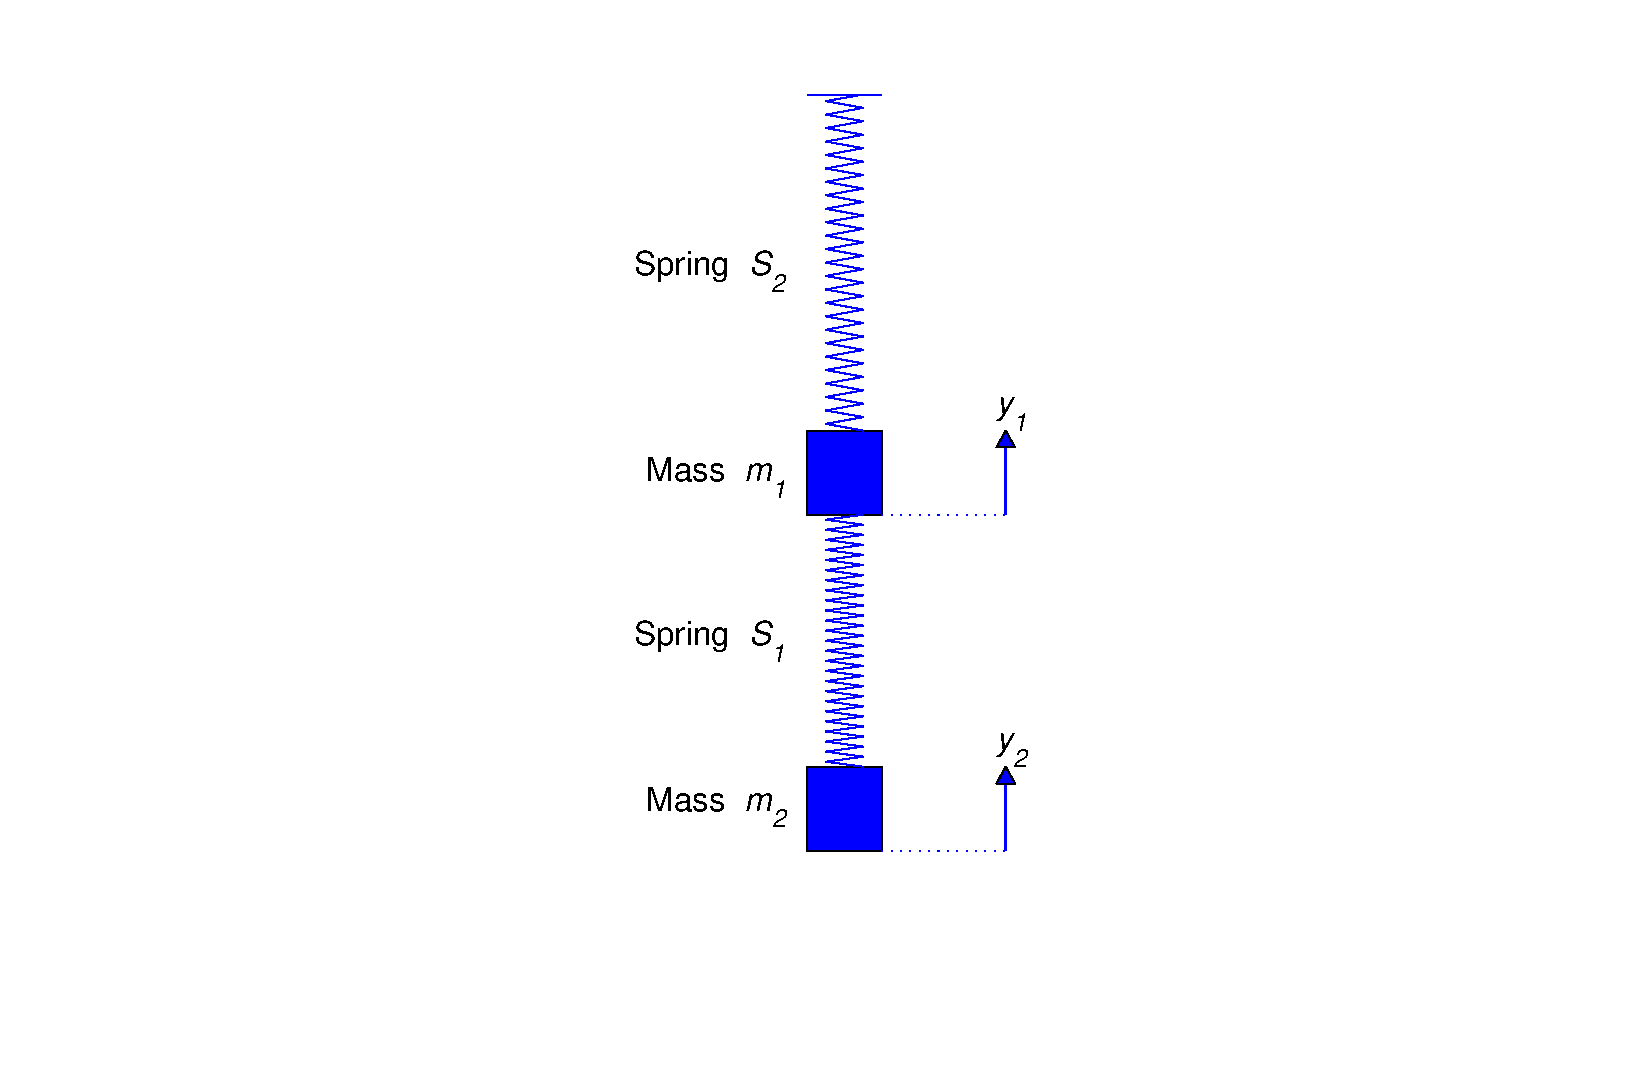
\includegraphics[bb=-78 148 689 643, width=5.67in, height=3.66in, keepaspectratio]{fig100102}
  \caption{}
  \label{figure:10.1.2}
\end{figure}

Let $H_{1}$ be the Hooke's law force acting on $m_{1}$, and let $D_{1}$ be the damping force on
$m_{1}$. Similarly, let $H_{2}$ and $D_{2}$ be the Hooke's law and damping forces acting on $m_{2}$.
According to Newton's second law of motion,
\begin{equation}
  \label{eq:10.1.8}
  \begin{array}{ccl}
    m_{1}y_{1}''=-m_{1}g+H_{1}+D_{1}+F_{1}, \\[1\jot]
    m_{2}y_{2}''=-m_{2}g+H_{2}+D_{2}+F_{2}.
  \end{array}
\end{equation}
When the displacements are $y_{1}$ and $y_{2}$, the change in length of $S_{1}$ is
$-y_{1}+\Delta\ell_{1}$ and the change in length of $S_{2}$ is $-y_{2}+y_{1}+\Delta\ell_{2}$. Both
springs exert Hooke's law forces on $m_{1}$, while only $S_{2}$ exerts a Hooke's law force on
$m_{2}$. These forces are in directions that tend to restore the springs to their natural lengths.
Therefore
\begin{equation}
  \label{eq:10.1.9}H_{1}=k_{1}(-y_{1}+\Delta\ell_{1})-k_{2}(-y_{2}+y_{1}+\Delta\ell_{2})\quad\mbox{ and }\quad H_{2}=k_{2}(-y_{2}+y_{1}+\Delta\ell_{2}).
\end{equation}
When the velocities are $y_{1}'$ and $y_{2}'$, $S_{1}$ and $S_{2}$ are changing length at the rates
$-y_{1}'$ and $-y_{2}'+y_{1}'$, respectively. Both springs exert damping forces on $m_{1}$, while
only $S_{2}$ exerts a damping force on $m_{2}$. Since the force due to damping exerted by a spring
is proportional to the rate of change of length of the spring and in a direction that opposes the
change, it follows that
\begin{equation}
  \label{eq:10.1.10}D_{1}=-c_{1}y_{1}'+c_{2}(y_{2}'-y_{1}')\quad\mbox{ and }\quad D_{2}=-c_{2}(y_{2}'-y_{1}').
\end{equation}

From \eqref{eq:10.1.8}, \eqref{eq:10.1.9}, and \eqref{eq:10.1.10},
\begin{equation}
  \label{eq:10.1.11}
  \begin{array}{ccl}
    m_{1}y_{1}'' & =       & -m_{1}g+k_{1}(-y_{1}+\Delta\ell_{1})-k_{2}(-y_{2}+y_{1}+\Delta\ell_{2})         \\[1\jot]
                 & \mbox{} & -c_{1}y_{1}'+c_{2}(y_{2}'-y_{1}')+F_{1}                                         \\[1\jot]
                 & =       & -(m_{1}g-k_{1}\Delta\ell_{1}+k_{2}\Delta\ell_{2})-k_{1}y_{1}+k_{2}(y_{2}-y_{1}) \\[1\jot]
                 & \mbox{} & -c_{1}y_{1}'+c_{2}(y_{2}'-y_{1}')+F_{1}
  \end{array}
\end{equation}
and
\begin{equation}
  \label{eq:10.1.12}
  \begin{array}{ccl}
    m_{2}y_{2}'' & = & -m_{2}g+k_{2}(-y_{2}+y_{1}+\Delta\ell_{2})-c_{2}(y_{2}'-y_{1}')+F_{2}        \\[1\jot]
                 & = & -(m_{2}g-k_{2}\Delta\ell_{2})-k_{2}(y_{2}-y_{1})-c_{2}(y_{2}'-y_{1}')+F_{2}.
  \end{array}
\end{equation}
From \eqref{eq:10.1.7},
\[
  m_{1}g-k_{1}\Delta\ell_{1}+k_{2}\Delta\ell_{2}=-m_{2}g+k_{2}\Delta\ell_{2}=0.
\]
Therefore we can rewrite \eqref{eq:10.1.11} and \eqref{eq:10.1.12} as
\begin{eqnarray*}
  m_{1}y_{1}'' & = & -(c_{1}+c_{2})y_{1}'+c_{2}y_{2}'-(k_{1}+k_{2})y_{1}+k_{2}y_{2}+F_{1} \\
  m_{2}y_{2}'' & = & c_{2}y_{1}'-c_{2}y_{2}'+k_{2}y_{1}-k_{2}y_{2}+F_{2}.\quad\bbox
\end{eqnarray*}

\begin{example}
  \label{example:10.1.3} \rm Let ${\bf X}={\bf X}(t)=x(t)\,{\bf i}+y(t)\,{\bf j}+z(t)\,{\bf k}$ be
  the position vector at time $t$ of an object with mass $m$, relative to a rectangular coordinate
  system with origin at Earth's center (Figure~\ref{figure:10.1.3}). According to Newton's law of
  gravitation, Earth's gravitational force ${\bf F}={\bf F}(x,y,z)$ on the object is inversely
  proportional to the square of the distance of the object from Earth's center, and directed toward
  the center; thus,
  \begin{equation}
    \label{eq:10.1.13}{\bf F}=\frac{K}{\|{\bf X}\|^{2}}\left(-\frac{{\bf X}}{\|{\bf X}\|}\right)=-K\frac{x\,{\bf i}+y\,{\bf j}+z\,{\bf k}}{\mbox{}\left(x^{2}+y^{2}+z^{2}\right)^{3/2}},
  \end{equation}
  where $K$ is a constant. To determine $K$, we observe that the magnitude of ${\bf F}$ is
  \[
    \|{\bf F}\|=K\frac{\|{\bf X}\|}{\|{\bf X}\|^{3}}=\frac{K}{\|{\bf X}\|^{2}}=\frac{K}{(x^{2}+y^{2}+z^{2})}.
  \]
  Let $R$ be Earth's radius. Since $\|{\bf F}\|=mg$ when the object is at Earth's surface,
  \[
    mg=\frac{K}{R^{2}},\quad\mbox{ so }\quad K=mgR^{2}.
  \]
  Therefore we can rewrite \eqref{eq:10.1.13} as
  \[
    {\bf F}=-mgR^{2}\frac{x\,{\bf i}+y\,{\bf j}+z\,{\bf k}}{\mbox{}\left(x^{2}+y^{2}+z^{2}\right)^{3/2}}.
  \]
  Now suppose ${\bf F}$ is the only force acting on the object. According to Newton's second law of
  motion, ${\bf F}=m{\bf X}''$; that is,
  \[
    m(x''\,{\bf i}+y''\,{\bf j}+z''\,{\bf k})= -mgR^{2}\frac{x\,{\bf i}+y\,{\bf j}+z\,{\bf k}}{\left(x^{2}+y^{2}+z^{2}\right)^{3/2}}.
  \]
  Cancelling the common factor $m$ and equating components on the two sides of this equation yields
  the system
  \begin{equation}
    \label{eq:10.1.14}
    \begin{array}{rcl}
      x'' & = & -\dst\frac{gR^{2}x}{(x^{2}+y^{2}+z^{2})^{3/2}}  \\[2\jot]
      y'' & = & -\dst\frac{gR^{2}y}{(x^{2}+y^{2}+z^{2})^{3/2}}  \\[2\jot]
      z'' & = & -\dst\frac{gR^{2}z}{(x^{2}+y^{2}+z^{2})^{3/2}}.
    \end{array}
  \end{equation}
\end{example}

\begin{figure}[tbp]
  \centering
  \color{blue}
  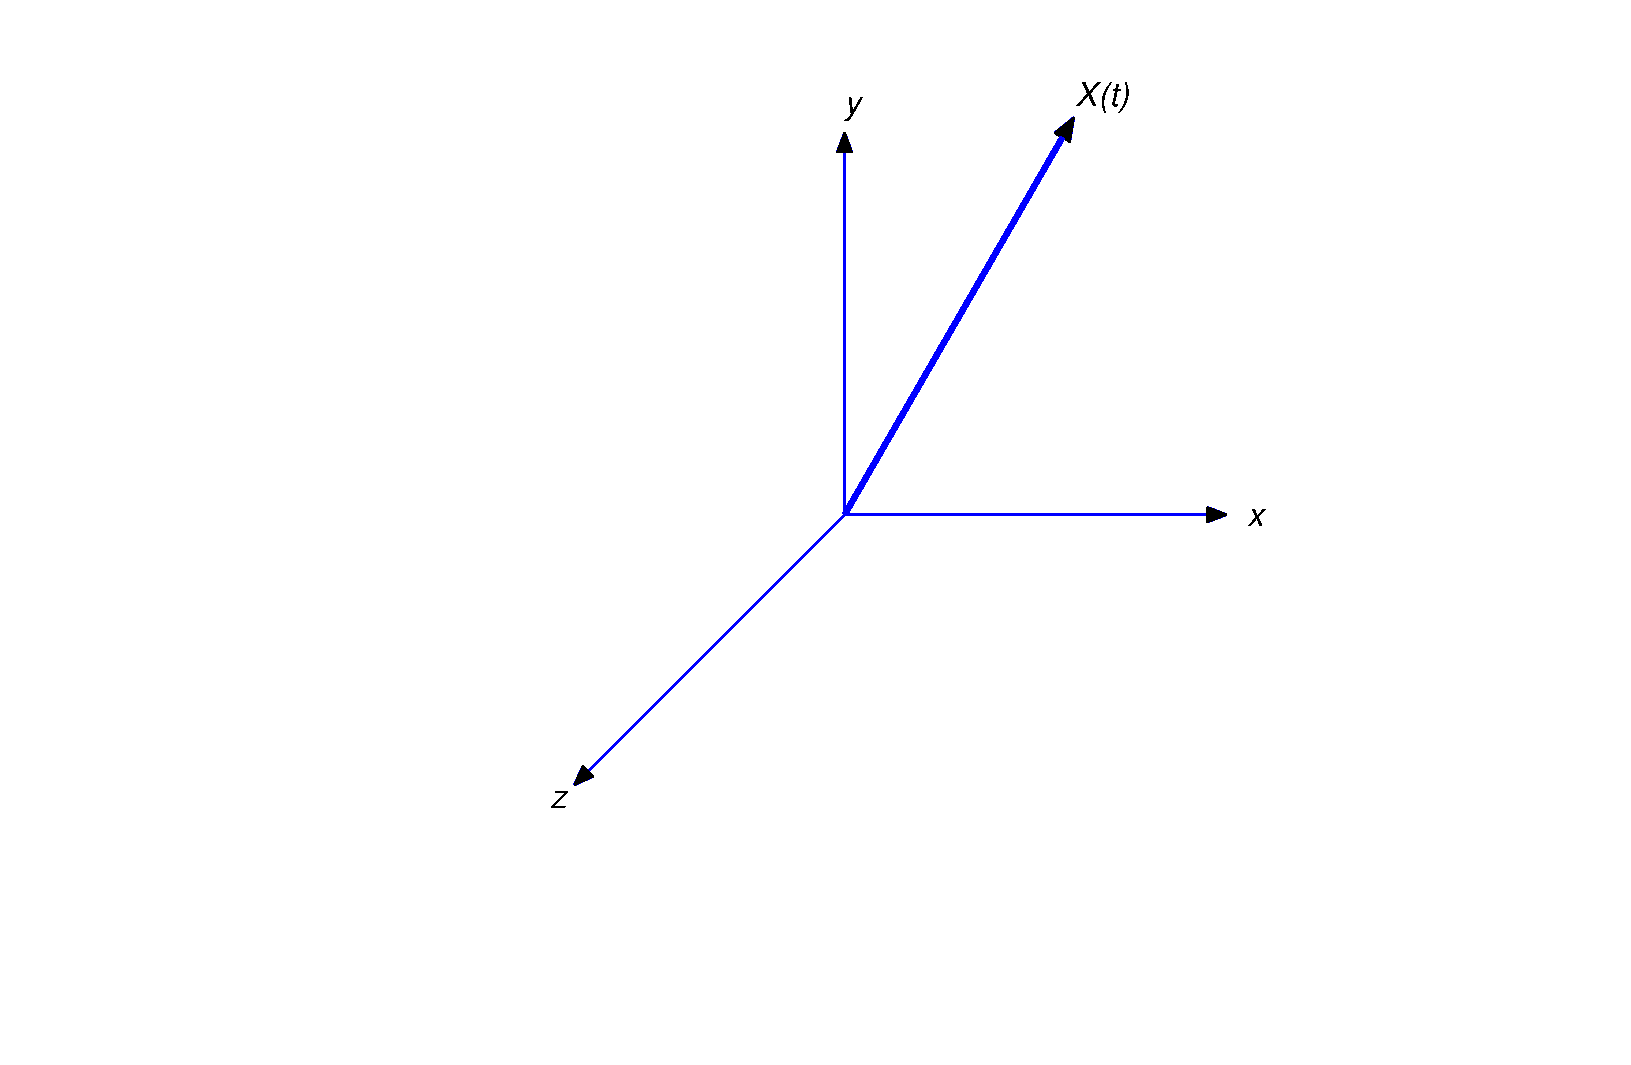
\includegraphics[bb=-78 148 689 643, width=5.67in, height=3.66in, keepaspectratio]{fig100103}
  \caption{}
  \label{figure:10.1.3}
\end{figure}

\boxit{Rewriting Higher Order Systems as First Order Systems}

\noindent
A system of the form
\begin{equation}
  \label{eq:10.1.15}
  \begin{array}{ccl}
    y_{1}' & =      & g_{1}(t,y_{1},y_{2},\dots,y_{n}) \\
    y_{2}' & =      & g_{2}(t,y_{1},y_{2},\dots,y_{n}) \\
           & \vdots &                                  \\
    y_{n}' & =      & g_{n}(t,y_{1},y_{2},\dots,y_{n})
  \end{array}
\end{equation}
is called a {\color{blue}\it first order system\/}, since the only derivatives occurring in it are
first derivatives. The derivative of each of the unknowns may depend upon the independent variable
and all the unknowns, but not on the derivatives of other unknowns. When we wish to emphasize the
number of unknown functions in \eqref{eq:10.1.15} we will say that \eqref{eq:10.1.15} is an
$n\times n$ system.

Systems involving higher order derivatives can often be reformulated as first order systems by
introducing additional unknowns. The next two examples illustrate this.

\begin{example}
  \label{example:10.1.4} \rm Rewrite the system
  \begin{equation}
    \label{eq:10.1.16}
    \begin{array}{rcl}
      m_{1}y_{1}'' & = & -(c_{1}+c_{2})y_{1}'+c_{2}y_{2}'-(k_{1}+k_{2})y_{1}+k_{2}y_{2}+F_{1} \\[1\jot]
      m_{2}y_{2}'' & = & c_{2}y_{1}'-c_{2}y_{2}'+k_{2}y_{1}-k_{2}y_{2}+F_{2}.
    \end{array}
  \end{equation}
  derived in Example~\ref{example:10.1.2} as a system of first order equations.
\end{example}

\solution{} If we define $v_{1}=y_{1}'$ and $v_{2}=y_{2}'$, then $v_{1}'=y_{1}''$ and
$v_{2}'=y_{2}''$, so \eqref{eq:10.1.16} becomes
\[
  \begin{array}{rcl}
    m_{1}v_{1}' & = & -(c_{1}+c_{2})v_{1}+c_{2}v_{2}-(k_{1}+k_{2})y_{1}+k_{2}y_{2}+F_{1} \\[1\jot]
    m_{2}v_{2}' & = & c_{2}v_{1}-c_{2}v_{2}+k_{2}y_{1}-k_{2}y_{2}+F_{2}.
  \end{array}
\]
Therefore $\{y_{1},y_{2},v_{1},v_{2}\}$ satisfies the $4\times4$ first order system
\begin{equation}
  \label{eq:10.1.17}
  \begin{array}{rcl}
    y_{1}' & = & v_{1}                                                                                              \\[1\jot]
    y_{2}' & = & v_{2}                                                                                              \\[1\jot]
    v_{1}' & = & \dst\frac{1}{m_{1}}\left[-(c_{1}+c_{2})v_{1}+c_{2}v_{2}-(k_{1}+k_{2})y_{1}+k_{2}y_{2}+F_{1}\right] \\[1\jot]
    v_{2}' & = & \dst\frac{1}{m_{2}}\left[c_{2}v_{1}-c_{2}v_{2}+k_{2}y_{1}-k_{2}y_{2}+F_{2}\right].
  \end{array}
\end{equation}

\color{blue}
\remark{ The difference in form between \eqref{eq:10.1.15} and \eqref{eq:10.1.17}, due to the way in
which the unknowns are {\color{blue}\it denoted} in the two systems, isn't important;
\eqref{eq:10.1.17} is a first order system, in that each equation in \eqref{eq:10.1.17} expresses
the first derivative of one of the unknown functions in a way that does not involve derivatives of
any of the other unknowns.}
\color{black}

\begin{example}
  \label{example:10.1.5} \rm Rewrite the system
  \[
    \begin{array}{ccc}
      x''  & = & f(t,x,x',y,y',y'') \\[1\jot]
      y''' & = & g(t,x,x',y,y',y'')
    \end{array}
  \]
  as a first order system.
\end{example}

\solution We regard $x$, $x'$, $y$, $y'$, and $y''$ as unknown functions, and rename them
\[
  x=x_{1},\;x'=x_{2},\quad y=y_{1},\quad y'=y_{2},\quad y''=y_{3}.
\]
These unknowns satisfy the system
\[
  \begin{array}{ccl}
    x_{1}' & = & x_{2}                               \\[1\jot]
    x_{2}' & = & f(t,x_{1},x_{2},y_{1},y_{2},y_{3})  \\[1\jot]
    y_{1}' & = & y_{2}                               \\[1\jot]
    y_{2}' & = & y_{3}                               \\[1\jot]
    y_{3}' & = & g(t,x_{1},x_{2},y_{1},y_{2},y_{3}).
  \end{array}
\]

\boxit{Rewriting Scalar Differential Equations as Systems}

\noindent
In this chapter we'll refer to differential equations involving only one unknown function as
{\color{blue}\it scalar\/} differential equations. Scalar differential equations can be rewritten as
systems of first order equations by the method illustrated in the next two examples.

\begin{example}
  \label{example:10.1.6} \rm Rewrite the equation
  \begin{equation}
    \label{eq:10.1.18}y^{(4)}+4y'''+6y''+4y'+y=0
  \end{equation}
  as a $4\times4$ first order system.
\end{example}

\solution We regard $y$, $y'$, $y''$, and $y'''$ as unknowns and rename them
\[
  y=y_{1},\quad y'=y_{2},\quad y''=y_{3},\mbox{\quad and \quad}y'''=y_{4}.
\]
Then $y^{(4)}=y_{4}'$, so \eqref{eq:10.1.18} can be written as
\[
  y_{4}'+4y_{4}+6y_{3}+4y_{2}+y_{1}=0.
\]
Therefore $\{y_{1},y_{2},y_{3},y_{4}\}$ satisfies the system
\begin{eqnarray*}
  y_{1}' & = & y_{2} \\
  y_{2}' & = & y_{3} \\
  y_{3}' & = & y_{4} \\
  y_{4}' & = & -4y_{4}-6y_{3}-4y_{2}-y_{1}.\bbox
\end{eqnarray*}

\begin{example}
  \label{example:10.1.7} \rm Rewrite
  \[
    x'''=f(t,x,x',x'')
  \]
  as a system of first order equations.
\end{example}

\solution We regard $x$, $x'$, and $x''$ as unknowns and rename them
\[
  x=y_{1},\quad x'=y_{2},\mbox{\quad and \quad}x''=y_{3}.
\]
Then
\[
  y_{1}'=x'=y_{2},\quad y_{2}'=x''=y_{3},\mbox{\quad and \quad}y_{3}'=x'''.
\]
Therefore $\{y_{1},y_{2},y_{3}\}$ satisfies the first order system
\[
  \begin{array}{ccl}
    y_{1}' & = & y_{2}                   \\[2\jot]
    y_{2}' & = & y_{3}                   \\[1\jot]
    y_{3}' & = & f(t,y_{1},y_{2},y_{3}).
  \end{array}
\]

Since systems of differential equations involving higher derivatives can be rewritten as first order
systems by the method used in Examples~\ref{example:10.1.5} --\ref{example:10.1.7} , we'll consider
only first order systems.

\boxit{Numerical Solution of Systems}

\noindent
The numerical methods that we studied in Chapter~3 can be extended to systems, and most differential
equation software packages include programs to solve systems of equations. We won't go into detail
on numerical methods for systems; however, for illustrative purposes we'll describe the Runge-Kutta
method for the numerical solution of the initial value problem
\begin{eqnarray*}
  y_{1}' & = & g_{1}(t,y_{1},y_{2}),\quad y_{1}(t_{0})=y_{10}, \\
  y_{2}' & = & g_{2}(t,y_{1},y_{2}),\quad y_{2}(t_{0})=y_{20}
\end{eqnarray*}
at equally spaced points $t_{0}$, $t_{1}$, \dots, $t_{n}=b$ in an interval $[t_{0},b]$. Thus,
\[
  t_{i}=t_{0}+ih,\quad i=0,1,\dots,n,
\]
where
\[
  h=\frac{b-t_{0}}{n}.
\]
We'll denote the approximate values of $y_{1}$ and $y_{2}$ at these points by
$y_{10},y_{11},\dots,y_{1n}$ and $y_{20},y_{21},\dots,y_{2n}$. The Runge-Kutta method computes these
approximate values as follows: given $y_{1i}$ and $y_{2i}$, compute
\begin{eqnarray*}
  I_{1i} & = & g_{1}(t_{i},y_{1i},y_{2i}),                                                            \\
  J_{1i} & = & g_{2}(t_{i},y_{1i},y_{2i}),                                                            \\
  I_{2i} & = & g_{1}\left(t_{i}+\frac{h}{2},y_{1i}+\frac{h}{2}I_{1i},y_{2i}+\frac{h}{2}J_{1i}\right), \\
  J_{2i} & = & g_{2}\left(t_{i}+\frac{h}{2},y_{1i}+\frac{h}{2}I_{1i},y_{2i}+\frac{h}{2}J_{1i}\right), \\
  I_{3i} & = & g_{1}\left(t_{i}+\frac{h}{2},y_{1i}+\frac{h}{2}I_{2i},y_{2i}+\frac{h}{2}J_{2i}\right), \\
  J_{3i} & = & g_{2}\left(t_{i}+\frac{h}{2},y_{1i}+\frac{h}{2}I_{2i},y_{2i}+\frac{h}{2}J_{2i}\right), \\
  I_{4i} & = & g_{1}(t_{i}+h,y_{1i}+hI_{3i},y_{2i}+hJ_{3i}),                                          \\
  J_{4i} & = & g_{2}(t_{i}+h,y_{1i}+hI_{3i},y_{2i}+hJ_{3i}),
\end{eqnarray*}
and
\begin{eqnarray*}
  y_{1,i+1} & = & y_{1i}+\frac{h}{6}(I_{1i}+2I_{2i}+2I_{3i}+I_{4i}), \\
  y_{2,i+1} & = & y_{2i}+\frac{h}{6}(J_{1i}+2J_{2i}+2J_{3i}+J_{4i})
\end{eqnarray*}
for $i=0$, \dots, $n-1$. Under appropriate conditions on $g_{1}$ and $g_{2}$, it can be shown that
the global truncation error for the Runge-Kutta method is $O(h^{4})$, as in the scalar case
considered in Section~3.3.

\exercises

\begin{exerciselist}
  \item\label{exer:10.1.1} Tanks $T_{1}$ and $T_{2}$ contain 50 gallons and 100 gallons of salt
        solutions, respectively. A solution with 2 pounds of salt per gallon is pumped into $T_{1}$
        from an external source at $1$~gal/min, and a solution with $3$ pounds of salt per gallon is
        pumped into $T_{2}$ from an external source at $2$~gal/min. The solution from $T_{1}$ is
        pumped into $T_{2}$ at $3$ gal/min, and the solution from $T_{2}$ is pumped into $T_{1}$ at
        $4$ gal/min. $T_{1}$ is drained at $2$~gal/min and $T_{2}$ is drained at $1$~gal/min. Let
        $Q_{1}(t)$ and $Q_{2}(t)$ be the number of pounds of salt in $T_{1}$ and $T_{2}$,
        respectively, at time $t>0$. Derive a system of differential equations for $Q_{1}$ and
        $Q_{2}$. Assume that both mixtures are well stirred.

  \item\label{exer:10.1.2} Two 500 gallon tanks $T_{1}$ and $T_{2}$ initially contain 100 gallons
        each of salt solution. A solution with $2$ pounds of salt per gallon is pumped into $T_{1}$
        from an external source at $6$~gal/min, and a solution with $1$ pound of salt per gallon is
        pumped into $T_{2}$ from an external source at $5$~gal/min. The solution from $T_{1}$ is
        pumped into $T_{2}$ at $2$ gal/min, and the solution from $T_{2}$ is pumped into $T_{1}$ at
        $1$ gal/min. Both tanks are drained at $3$~gal/min. Let $Q_{1}(t)$ and $Q_{2}(t)$ be the
        number of pounds of salt in $T_{1}$ and $T_{2}$, respectively, at time $t>0$. Derive a
        system of differential equations for $Q_{1}$ and $Q_{2}$ that's valid until a tank is about
        to overflow. Assume that both mixtures are well stirred.

  \item\label{exer:10.1.3} A mass $m_{1}$ is suspended from a rigid support on a spring $S_{1}$ with
        spring constant $k_{1}$ and damping constant $c_{1}$. A second mass $m_{2}$ is suspended
        from the first on a spring $S_{2}$ with spring constant $k_{2}$ and damping constant
        $c_{2}$, and a third mass $m_{3}$ is suspended from the second on a spring $S_{3}$ with
        spring constant $k_{3}$ and damping constant $c_{3}$. Let $y_{1}=y_{1}(t)$,
        $y_{2}=y_{2}(t)$, and $y_{3}=y_{3}(t)$ be the displacements of the three masses from their
        equilibrium positions at time $t$, measured positive upward. Derive a system of differential
        equations for $y_{1}$, $y_{2}$ and $y_{3}$, assuming that the masses of the springs are
        negligible and that vertical external forces $F_{1}$, $F_{2}$, and $F_{3}$ also act on the
        masses.

  \item\label{exer:10.1.4} Let ${\bf X}=x\,{\bf i}+y\,{\bf j}+z\,{\bf k}$ be the position vector of
        an object with mass $m$, expressed in terms of a rectangular coordinate system with origin
        at Earth's center (Figure~\ref{figure:10.1.3}). Derive a system of differential equations
        for $x$, $y$, and $z$, assuming that the object moves under Earth's gravitational force
        (given by Newton's law of gravitation, as in Example~\ref{example:10.1.3} ) and a resistive
        force proportional to the speed of the object. Let $\alpha$ be the constant of
        proportionality.

  \item\label{exer:10.1.5} Rewrite the given system as a first order system.

  \begin{tabular}[t]{@{}p{168pt}@{}p{168pt}}
    ${\bf(a)}\begin{array}{lcc}x'''=f(t,x,y,y')\\[1\jot]y''= g(t,y,y')\end{array}$ & {\bf (b)}$\begin{array}{lcl}u'= f(t,u,v,v',w')\\[1\jot]v''=g(t,u,v,v',w) \\[1\jot]w''=h(t,u,v,v',w,w')\end{array}$ \\[30pt]
    {\bf (c)} $y'''= f(t,y,y',y'')$                                                & {\bf (d)} $y^{(4)}=f(t,y)$                                                                                         \\[20pt]
    {\bf (e)}$\begin{array}{lcc}x''=f(t,x,y)\\[1\jot]y''= g(t,x,y)\end{array}$
  \end{tabular}

  \item\label{exer:10.1.6} Rewrite the system \eqref{eq:10.1.14} of differential equations derived
        in Example~\ref{example:10.1.3} as a first order system.

  \item\label{exer:10.1.7} Formulate a version of Euler's method (Section~3.1) for the numerical
        solution of the initial value problem
  \[
    \begin{array}{rcl}
      y_{1}' & = & g_{1}(t,y_{1},y_{2}),\quad y_{1}(t_{0})=y_{10}, \\
      y_{2}' & = & g_{2}(t,y_{1},y_{2}),\quad y_{2}(t_{0})=y_{20},
    \end{array}
  \]
  on an interval $[t_{0},b]$.

  \item\label{exer:10.1.8} Formulate a version of the improved Euler method (Section~3.2) for the
        numerical solution of the initial value problem
  \[
    \begin{array}{rcl}
      y_{1}' & = & g_{1}(t,y_{1},y_{2}),\quad y_{1}(t_{0})=y_{10}, \\
      y_{2}' & = & g_{2}(t,y_{1},y_{2}),\quad y_{2}(t_{0})=y_{20},
    \end{array}
  \]
  on an interval $[t_{0},b]$.
\end{exerciselist}


\section{Linear Systems of Differential Equations}

\noindent
A first order system of differential equations that can be written in the form
\begin{equation}
  \label{eq:10.2.1}
  \begin{array}{ccl}
    y'_{1} & =     & a_{11}(t)y_{1}+a_{12}(t)y_{2}+\cdots+a_{1n}(t)y_{n}+f_{1}(t) \\
    y'_{2} & =     & a_{21}(t)y_{1}+a_{22}(t)y_{2}+\cdots+a_{2n}(t)y_{n}+f_{2}(t) \\
           & \vdots \\
    y'_{n} & =     & a_{n1}(t)y_{1}+a_{n2}(t)y_{2}+\cdots+a_{nn}(t)y_{n}+f_{n}(t)
  \end{array}
\end{equation}
is called a {\color{blue}\it linear system\/}.

The linear system \eqref{eq:10.2.1} can be written in matrix form as
\[
  \col{y'}n=\matfunc ann\col yn+\colfunc fn,
\]
or more briefly as
\begin{equation}
  \label{eq:10.2.2}{\bf y}'=A(t){\bf y}+{\bf f}(t),
\end{equation}
where
\[
  {\bf y}=\col yn,\quad A(t)=\matfunc ann,\mbox{\quad and \quad}{\bf f}(t)=\colfunc fn.
\]
We call $A$ the {\color{blue}\it coefficient matrix\/} of \eqref{eq:10.2.2} and ${\bf f}$ the
{\color{blue}\it forcing function\/}. We'll say that $A$ and ${\bf f}$ are {\color{blue}\it
continuous\/} if their entries are continuous. If ${\bf f}={\bf0}$, then \eqref{eq:10.2.2} is
{\color{blue}\it homogeneous\/}; otherwise, \eqref{eq:10.2.2} is {\color{blue}\it nonhomogeneous\/}.

An initial value problem for \eqref{eq:10.2.2} consists of finding a solution of \eqref{eq:10.2.2}
that equals a given constant vector
\[
  {\bf k}=\col kn.
\]
at some initial point $t_{0}$. We write this initial value problem as
\[
  {\bf y}'=A(t){\bf y}+{\bf f}(t),\quad{\bf y}(t_{0})={\bf k}.
\]

The next theorem gives sufficient conditions for the existence of solutions of initial value
problems for \eqref{eq:10.2.2}. We omit the proof.

\begin{theorem}
  \color{blue}
  \label{thmtype:10.2.1} Suppose the coefficient matrix $A$ and the forcing function ${\bf f}$ are
  continuous on $(a,b)$, let $t_{0}$ be in $(a,b)$, and let ${\bf k}$ be an arbitrary constant
  $n$-vector. Then the initial value problem
  \[
    {\bf y}'=A(t){\bf y}+{\bf f}(t),\quad{\bf y}(t_{0})={\bf k}
  \]
  has a unique solution on $(a,b)$.
\end{theorem}

\begin{example}
  \label{example:10.2.1} \rm \mbox{}
  \newline
  \begin{alist}
    \item % (a)
    Write the system
    \begin{equation}
      \label{eq:10.2.3}
      \begin{array}{rcl}
        y_{1}' & = & \phantom{2}y_{1}+2y_{2}+2e^{4t}           \\[1\jot]
        y_{2}' & = & 2y_{1}+\phantom{2}y_{2}+\phantom{2}e^{4t}
      \end{array}
    \end{equation}
    in matrix form and conclude from Theorem~\ref{thmtype:10.2.1} that every initial value problem
    for \eqref{eq:10.2.3} has a unique solution on $(-\infty,\infty)$.

    \item % (b)
    Verify that
    \begin{equation}
      \label{eq:10.2.4}{\bf y}= \frac{1}{5}\twocol87e^{4t}+c_{1}\twocol11e^{3t}+c_{2}\twocol1{-1}e^{-t}
    \end{equation}
    is a solution of \eqref{eq:10.2.3} for all values of the constants $c_{1}$ and $c_{2}$.

    \item % (c)
    Find the solution of the initial value problem
    \begin{equation}
      \label{eq:10.2.5}{\bf y}'=\twobytwo1221{\bf y}+\twocol21e^{4t},\quad{\bf y}(0)=\frac{1}{5}\twocol3{22}.
    \end{equation}
  \end{alist}
\end{example}

\solutionpart{a} The system \eqref{eq:10.2.3} can be written in matrix form as
\[
  {\bf y}'=\twobytwo1221{\bf y}+\twocol21e^{4t}.
\]
An initial value problem for \eqref{eq:10.2.3} can be written as
\[
  {\bf y}'=\twobytwo1221{\bf y}+\twocol21e^{4t},\quad y(t_{0})=\twocol{k_{1}}{k_{2}}.
\]
Since the coefficient matrix and the forcing function are both continuous on $(-\infty,\infty)$,
Theorem~\ref{thmtype:10.2.1} implies that this problem has a unique solution on $(-\infty,\infty)$.

\solutionpart{b} If ${\bf y}$ is given by \eqref{eq:10.2.4}, then
\begin{eqnarray*}
  A{\bf y}+{\bf f} & = & \frac{1}{5}\twobytwo1221\twocol87e^{4t}+c_{1}\twobytwo1221\twocol11e^{3t}                     \\[2\jot]
                   &   & +c_{2}\twobytwo1221\twocol1{-1}e^{-t}+\twocol21e^{4t}                                         \\[2\jot]
                   & = & \frac{1}{5}\twocol{22}{23}e^{4t}+c_{1}\twocol33e^{3t}+c_{2}\twocol{-1}1e^{-t}+\twocol21e^{4t} \\[2\jot]
                   & = & \frac{1}{5}\twocol{32}{28}e^{4t}+3c_{1}\twocol11e^{3t}-c_{2}\twocol1{-1}e^{-t}={\bf y}'.
\end{eqnarray*}

\solutionpart{c} We must choose $c_{1}$ and $c_{2}$ in \eqref{eq:10.2.4} so that
\[
  \frac{1}{5}\twocol87+c_{1}\twocol11+c_{2}\twocol1{-1}=\frac{1}{5}\twocol3{22},
\]
which is equivalent to
\[
  \twobytwo111{-1}\twocol{c_{1}}{c_{2}}=\twocol{-1}3.
\]
Solving this system yields $c_{1}=1$, $c_{2}=-2$, so
\[
  {\bf y}=\frac{1}{5}\twocol87e^{4t}+\twocol11e^{3t}-2\twocol1{-1}e^{-t}
\]
is the solution of \eqref{eq:10.2.5}.

\color{blue}
\remark{The theory of $n\times n$ linear systems of differential equations is analogous to the
theory of the scalar $n$-th order
equation \begin{equation}\label{eq:10.2.6}P_{0}(t)y^{(n)}+P_{1}(t)y^{(n-1)}+\cdots+P_{n}(t)y=F(t),\end{equation}
as developed in Sections~9.1. For example, by rewriting \eqref{eq:10.2.6} as an equivalent linear
system it can be shown that Theorem~\ref{thmtype:10.2.1} implies Theorem~\ref{thmtype:9.1.1}
(Exercise~\ref{exer:10.2.12}).}
\color{black}

\newpage
\exercises

\begin{exerciselist}
  \item\label{exer:10.2.1} Rewrite the system in matrix form and verify that the given vector
        function satisfies the system for any choice of the constants $c_{1}$ and $c_{2}$.

  \begin{alist}
    \item % (a)
    $\begin{array}{ccl}
      y'_{1} & = & 2y_{1}+4y_{2}  \\
      y_{2}' & = & 4y_{1}+2y_{2};
    \end{array}\quad{\bf y}=c_{1}\twocol11e^{6t}+c_{2}\twocol1{-1}e^{-2t}$

    \item % (b)
    $\begin{array}{ccl}
      y'_{1} & = & -2y_{1}-2y_{2}            \\
      y_{2}' & = & -5y_{1}+\phantom{2}y_{2};
    \end{array}\quad{\bf y}=c_{1}\twocol11e^{-4t}+c_{2}\twocol{-2}5e^{3t}$

    \item % (c)
    $\begin{array}{ccr}
      y'_{1} & = & -4y_{1}-10y_{2}           \\
      y_{2}' & = & 3y_{1}+\phantom{1}7y_{2};
    \end{array}\quad{\bf y}=c_{1}\twocol{-5}3e^{2t}+c_{2}\twocol2{-1}e^{t}$

    \item % (d)
    $\begin{array}{ccl}
      y'_{1} & = & 2y_{1}+\phantom{2}y_{2}  \\
      y_{2}' & = & \phantom{2}y_{1}+2y_{2};
    \end{array}\quad{\bf y}=c_{1}\twocol11e^{3t}+c_{2}\twocol1{-1}e^{t}$
  \end{alist}

  \item\label{exer:10.2.2} Rewrite the system in matrix form and verify that the given vector
        function satisfies the system for any choice of the constants $c_{1}$, $c_{2}$, and $c_{3}$.

  \begin{alist}
    \item % (a)
    $\begin{array}{ccr}
      y'_{1} & = & -y_{1}+2y_{2}+3y_{3} \\
      y_{2}' & = & y_{2}+6y_{3}         \\
      y_{3}' & = & -2y_{3};
    \end{array}$

    ${\bf y}=c_{1}\threecol110e^{t}+c_{2}\threecol100e^{-t}+c_{3}\threecol1{-2}1e^{-2t}$

    \item % (b)
    $\begin{array}{ccc}
      y'_{1} & = & \phantom{2y_{1}+}2y_{2}+2y_{3}   \\
      y_{2}' & = & 2y_{1}\phantom{+2y_{2}}+2y_{3}   \\
      y_{3}' & = & 2y_{1}+ 2y_{2};\phantom{+2y_{3}}
    \end{array}$

    ${\bf y}=c_{1}\threecol{-1}01e^{-2t}+c_{2}\threecol0{-1}1e^{-2t}+c_{3}\threecol111e^{4t}$

    \item % (c)
    $\begin{array}{ccr}
      y'_{1} & = & -y_{1}+2y_{2}+2y_{3}             \\
      y_{2}' & = & 2y_{1}-\phantom{2}y_{2}+2y_{3}   \\
      y_{3}' & = & 2y_{1}+2y_{2} -\phantom{2}y_{3};
    \end{array}$

    ${\bf y}=c_{1}\threecol{-1}01e^{-3t}+c_{2}\threecol0{-1}1e^{-3t}+c_{3}\threecol111e^{3t}$

    \item % (d)
    $\begin{array}{ccr}
      y'_{1} & = & 3y_{1}-\phantom{2}y_{2} -\phantom{2}y_{3}   \\
      y_{2}' & = & -2y_{1}+3y_{2}+2y_{3}                       \\
      y_{3}' & = & \phantom{-}4y_{1}-\phantom{3}y_{2}- 2y_{3};
    \end{array}$

    ${\bf y}=c_{1}\threecol101e^{2t}+c_{2}\threecol1{-1}1e^{3t}+c_{3}\threecol1{-3}7e^{-t}$
  \end{alist}

  \item\label{exer:10.2.3} Rewrite the initial value problem in matrix form and verify that the
        given vector function is a solution.

  \begin{alist}
    \item % (a)
    $\begin{array}{ccl}
      y'_{1} & = & \phantom{-2}y_{1}+\phantom{4}y_{2} \\
      y_{2}' & = & -2y_{1}+ 4y_{2},
    \end{array}
    \begin{array}{ccr}
      y_{1}(0) & = & 1  \\
      y_{2}(0) & = & 0;
    \end{array}$ \quad ${\bf y}=2\twocol11e^{2t}-\twocol12e^{3t}$

    \item % (b)
    $\begin{array}{ccl}
      y'_{1} & = & 5y_{1}+3y_{2} \\
      y_{2}' & = & -y_{1}+y_{2},
    \end{array}
    \begin{array}{ccr}
      y_{1}(0) & = & 12  \\
      y_{2}(0) & = & -6;
    \end{array}$ \quad ${\bf y}=3\twocol1{-1}e^{2t}+3\twocol3{-1}e^{4t}$
  \end{alist}

  \item\label{exer:10.2.4} Rewrite the initial value problem in matrix form and verify that the
        given vector function is a solution.

  \begin{alist}
    \item % (a)
    $\begin{array}{ccr}
      y'_{1} & = & 6y_{1}+4y_{2}+4y_{3}  \\
      y_{2}' & = & -7y_{1}-2y_{2}-y_{3}, \\
      y_{3}' & = & 7y_{1}+4y_{2}+3y_{3}
    \end{array},\;
    \begin{array}{ccr}
      y_{1}(0) & = & 3  \\
      y_{2}(0) & = & -6 \\
      y_{3}(0) & = & 4
    \end{array}$

    ${\bf y}=\threecol1{-1}1e^{6t}+2\threecol1{-2}1e^{2t}+\threecol0{-1}1e^{-t}$

    \item % (b)
    $\begin{array}{ccr}
      y'_{1} & = & \phantom{-}8y_{1}+7y_{2}+\phantom{1}7y_{3} \\
      y_{2}' & = & -5y_{1}-6y_{2}-\phantom{1}9y_{3},          \\
      y_{3}' & = & \phantom{-}5y_{1}+7y_{2}+10y_{3},
    \end{array}\
    \begin{array}{ccr}
      y_{1}(0) & = & 2  \\
      y_{2}(0) & = & -4 \\
      y_{3}(0) & = & 3
    \end{array}$

    ${\bf y}=\threecol1{-1}1e^{8t}+\threecol0{-1}1e^{3t}+\threecol1{-2}1e^{t}$
  \end{alist}

  \item\label{exer:10.2.5} Rewrite the system in matrix form and verify that the given vector
        function satisfies the system for any choice of the constants $c_{1}$ and $c_{2}$.

  \begin{alist}
    \item % (a)
    $\begin{array}{ccc}
      y'_{1} & = & -3y_{1}+2y_{2}+3-2t \\
      y_{2}' & = & -5y_{1}+3y_{2}+6-3t
    \end{array}$

    ${\bf y}=c_{1}\left[
    \begin{array}{c}
      2\cos t        \\
      3\cos t-\sin t
    \end{array}\right]+c_{2}\left[
    \begin{array}{c}
      2\sin t        \\
      3\sin t+\cos t
    \end{array}\right]+\twocol1t$

    \item % (b)
    $\begin{array}{ccc}
      y'_{1} & = & 3y_{1}+y_{2}-5e^{t} \\
      y_{2}' & = & -y_{1}+y_{2}+e^{t}
    \end{array}$

    ${\bf y}=c_{1}\twocol{-1}1e^{2t}+c_{2}\left[
    \begin{array}{c}
      1+t \\
      -t
    \end{array}
    \right]e^{2t}+\twocol13e^{t}$

    \item % (c)
    $\begin{array}{ccl}
      y'_{1} & = & -y_{1}-4y_{2}+4e^{t}+8te^{t}               \\
      y_{2}' & = & -y_{1}-\phantom{4}y_{2}+e^{3t}+(4t+2)e^{t}
    \end{array}$

    ${\bf y}=c_{1}\twocol21e^{-3t}+c_{2}\twocol{-2}1e^{t}+\left[
    \begin{array}{c}
      e^{3t}  \\
      2te^{t}
    \end{array}\right]$

    \item % (d)
    $\begin{array}{ccc}
      y'_{1} & = & -6y_{1}-3y_{2}+14e^{2t}+12e^{t}         \\
      y_{2}' & = & \phantom{6}y_{1}-2y_{2}+7e^{2t}-12e^{t}
    \end{array}$

    ${\bf y}=c_{1}\twocol{-3}1e^{-5t}+c_{2}\twocol{-1}1e^{-3t}+ \left[
    \begin{array}{c}
      e^{2t}+3e^{t}  \\
      2e^{2t}-3e^{t}
    \end{array}\right]$
  \end{alist}

  \item\label{exer:10.2.6} Convert the linear scalar equation
  \[
    P_{0}(t)y^{(n)}+P_{1}(t)y^{(n-1)}+\cdots+P_{n}(t)y(t)=F(t) \eqno{\rm(A)}
  \]
  into an equivalent $n\times n$ system
  \[
    {\bf y'}=A(t){\bf y}+{\bf f}(t),
  \]
  and show that $A$ and ${\bf f}$ are continuous on an interval $(a,b)$ if and only if (A) is normal
  on $(a,b)$.

  \item\label{exer:10.2.7} A matrix function
  \[
    Q(t)=\matfunc qrs
  \]
  is said to be {\color{blue}\it differentiable\/} if its entries $\{q_{ij}\}$ are differentiable.
  Then the {\color{blue}\it derivative\/} $Q'$ is defined by
  \[
    Q'(t)=\matfunc{q'}rs.
  \]
  \begin{alist}
    \item % (a)
    Prove: If $P$ and $Q$ are differentiable matrices such that $P+Q$ is defined and if $c_{1}$ and
    $c_{2}$ are constants, then
    \[
      (c_{1}P+c_{2}Q)'=c_{1}P'+c_{2}Q'.
    \]

    \item % (b)
    Prove: If $P$ and $Q$ are differentiable matrices such that $PQ$ is defined, then
    \[
      (PQ)'=P'Q+PQ'.
    \]
  \end{alist}

  \item\label{exer:10.2.8} Verify that $Y'=AY$.

  \begin{alist}
    \item % (a)
    $\dst{Y=\twobytwo{e^{6t}}{e^{-2t}} {e^{6t}}{-e^{-2t}},\quad A=\twobytwo2 4 4 2}$

    \item % (b)
    $\dst{Y=\twobytwo{e^{-4t}} {-2e^{3t}}{e^{-4t}}{5e^{3t}},\quad A=\twobytwo{-2} {-2}{-5}{1}}$

    \item % (c)
    $\dst{Y=\twobytwo{-5e^{2t}} {2e^{t}}{3e^{2t}}{-e^{t}},\quad A= \twobytwo{-4}{-10}3 7}$

    \item % (d)
    $\dst{Y=\twobytwo{e^{3t}} {e^{t}}{e^{3t}}{-e^{t}},\quad A=\twobytwo2 1 1 2}$

    \item % (e)
    $Y=\left[
    \begin{array}{crr}
      e^{t} & e^{-t} & e^{-2t}   \\
      e^{t} & 0      & -2e^{-2t} \\
      0     & 0      & e^{-2t}
    \end{array}\right],\quad A=\threebythree{-1}2{3}{0}1 6 0 0{-2}$

    \item % (f)
    $\dst{Y=\cthreebythree{-e^{-2t}} {-e^{-2t}}{e^{4t}}0{\phantom{-}e^{-2t}}{e^{4t}} {e^{-2t}}0{e^{4t}},\quad A= \threebythree0 2 2 2 0 2 2 2 0}$

    \item % (g)
    $\dst{Y=\cthreebythree{e^{3t}} {e^{-3t}}0{e^{3t}}0{-e^{-3t}}{e^{3t}} {e^{-3t}}{\phantom{-}e^{-3t}},\quad A=\threebythree {-9}66{-6}36{-6}63}$

    \item % (h)
    $Y=\left[
    \begin{array}{crr}
      e^{2t} & e^{3t}  & e^{-t}   \\
      0      & -e^{3t} & -3e^{-t} \\
      e^{2t} & e^{3t}  & 7e^{-t}
    \end{array}\right], \quad A= \threebythree3{-1}{-1}{-2}3 2 4{-1}{-2}$
  \end{alist}

  \item\label{exer:10.2.9} Suppose
  \[
    {\bf y}_{1}=\twocol{y_{11}}{y_{21}}\mbox{\quad and \quad}{\bf y}_{2}=\twocol{y_{12}}{y_{22}}
  \]
  are solutions of the homogeneous system
  \[
    {\bf y}'=A(t){\bf y}, \eqno{\rm(A)}
  \]
  and define
  \enlargethispage{1in}
  \[
    Y= \twobytwo{y_{11}}{y_{12}}{y_{21}}{y_{22}}.
  \]
  \begin{alist}
    \item % (a)
    Show that $Y'=AY$.

    \item % (b)
    Show that if ${\bf c}$ is a constant vector then ${\bf y}= Y{\bf c}$ is a solution of (A).

    \item % (c)
    State generalizations of \part{a} and \part{b} for $n\times n$ systems.
  \end{alist}
  \newpage

  \item\label{exer:10.2.10} Suppose $Y$ is a differentiable square matrix.
  \begin{alist}
    \item % (a)
    Find a formula for the derivative of $Y^{2}$.

    \item % (b)
    Find a formula for the derivative of $Y^{n}$, where $n$ is any positive integer.

    \item % (c)
    State how the results obtained in \part{a} and \part{b} are analogous to results from calculus
    concerning scalar functions.
  \end{alist}

  \item\label{exer:10.2.11} It can be shown that if $Y$ is a differentiable and invertible square
        matrix function, then $Y^{-1}$ is differentiable.

  \begin{alist}
    \item % (a)
    Show that ($Y^{-1})'= -Y^{-1}Y'Y^{-1}$. (Hint: Differentiate the identity $Y^{-1}Y=I$.)

    \item % (b)
    Find the derivative of $Y^{-n}=\left(Y^{-1}\right)^{n}$, where $n$ is a positive integer.

    \item % (c)
    State how the results obtained in \part{a} and \part{b} are analogous to results from calculus
    concerning scalar functions.
  \end{alist}

  \item\label{exer:10.2.12} Show that Theorem~\ref{thmtype:10.2.1} implies
        Theorem~\ref{thmtype:9.1.1}. \hint{Write the scalar
        equation \[P_{0}(x)y^{(n)}+P_{1}(x)y^{(n-1)}+\cdots+P_{n}(x)y=F(x)\] as an $n\times n$
        system of linear equations.}

  \item\label{exer:10.2.13} Suppose ${\bf y}$ is a solution of the $n\times n$ system
        ${\bf y}'=A(t){\bf y}$ on $(a,b)$, and that the $n\times n$ matrix $P$ is invertible and
        differentiable on $(a,b)$. Find a matrix $B$ such that the function ${\bf x}=P{\bf y}$ is a
        solution of ${\bf x}'=B{\bf x}$ on $(a,b)$.
\end{exerciselist}


\newsection{3} {Linear Systems of Differential  Equations}
{Basic Theory of Homogeneous Linear System}
\currentpdfbookmark{Section 10.3 Basic Theory of Homogeneous Linear System}{section:10.3}
\vskip14pt

\renewcommand{\thissection}{\sectiontitle
{\,\quad BASIC THEORY OF HOMOGENEOUS LINEAR SYSTEMS}}
\thissection

\noindent
In this section we consider homogeneous linear systems ${\bf y}'=
A(t){\bf y}$, where $A=A(t)$ is a continuous $n\times n$ matrix
function on an interval $(a,b)$. The theory of linear homogeneous
systems has much in common with the theory of linear homogeneous
scalar equations, which we considered in
Sections~2.1, 5.1, and 9.1.

Whenever we refer to solutions of ${\bf y}'=A(t){\bf y}$ we'll mean
solutions on $(a,b)$. Since ${\bf y}\equiv{\bf 0}$ is obviously a
solution of ${\bf y}'=A(t){\bf y}$, we call it the {\color{blue}\it trivial\/}
solution. Any other solution is {\color{blue}\it nontrivial\/}.

If ${\bf y}_1$, ${\bf y}_2$, \dots, ${\bf y}_n$ are vector functions
defined on an interval $(a,b)$ and $c_1$, $c_2$, \dots, $c_n$ are
constants, then
\begin{equation} \label{eq:10.3.1}
{\bf y}=c_1{\bf y}_1+c_2{\bf y}_2+\cdots+c_n{\bf y}_n
\end{equation}
is a {\color{blue}\it linear combination of\/} ${\bf y}_1$, ${\bf y}_2$, \ldots,${\bf
y}_n$. It's easy show that if ${\bf
y}_1$, ${\bf y}_2$, \dots,${\bf y}_n$ are solutions of ${\bf y}'=A(t){\bf
y}$ on $(a,b)$, then so is any linear combination of
 ${\bf y}_1$, ${\bf y}_2$, \dots, ${\bf y}_n$ (Exercise~\ref{exer:10.3.1}). We say that
$\{{\bf y}_1,{\bf y}_2,\dots,{\bf y}_n\}$ is a {\color{blue}\it fundamental set of
solutions of ${\bf y}'=A(t){\bf y}$ on\/} $(a,b)$ on if every solution of
${\bf y}'=A(t){\bf y}$ on $(a,b)$ can be written as a linear combination of
${\bf y}_1$, ${\bf y}_2$, \dots, ${\bf y}_n$, as in \eqref{eq:10.3.1}.
In this
case we say that \eqref{eq:10.3.1} is the {\color{blue}\it general solution of ${\bf
y}'=A(t){\bf y}$ on\/} $(a,b)$.

It can be shown that if $A$ is continuous on $(a,b)$ then ${\bf
y}'=A(t){\bf y}$ has infinitely many fundamental sets of solutions on
$(a,b)$ (Exercises~\ref{exer:10.3.15} and \ref{exer:10.3.16}). The next
definition will help to characterize fundamental sets of solutions of
${\bf y}'=A(t){\bf y}$.

We say that a set $\{{\bf y}_1,{\bf y}_2,\dots,{\bf y}_n\}$ of
$n$-vector functions is {\color{blue}\it linearly independent\/} on $(a,b)$ if the
only constants $c_1$, $c_2$, \dots, $c_n$ such that
\begin{equation} \label{eq:10.3.2}
 c_1{\bf y}_1(t)+c_2{\bf y}_2(t)+\cdots+c_n{\bf y}_n(t)=0,\quad
a<t<b,
\end{equation}
are $c_1=c_2=\cdots=c_n=0$. If \eqref{eq:10.3.2} holds for some set of
constants $c_1$, $c_2$, \dots, $c_n$ that are not all zero, then $\{{\bf
y}_1,{\bf y}_2,\dots,{\bf y}_n\}$ is {\color{blue}\it linearly dependent\/} on
$(a,b)$

The next theorem is analogous to
Theorems~\ref{thmtype:5.1.3} and
\ref{thmtype:9.1.2}.

\begin{theorem}\color{blue}\label{thmtype:10.3.1}
Suppose the $n\times n$ matrix $A=A(t)$ is continuous on $(a,b)$.
Then a set
$\{{\bf y}_1,{\bf y}_2,\dots,{\bf y}_n\}$ of $n$ solutions of ${\bf
y}'=A(t){\bf y}$ on $(a,b)$ is a fundamental set if and only if it's
linearly independent on $(a,b)$.
\end{theorem}

\begin{example}\label{example:10.3.1} \rm
Show that the vector functions
$$
{\bf y}_1=\left[\begin{array}{c}e^t\\0\\e^{-t}\end{array}\right],\quad
{\bf
y}_2=\left[\begin{array}{c}0\\e^{3t}\\1\end{array}\right],
\mbox{\quad and \quad}{\bf
y}_3=\left[\begin{array}{c}e^{2t}\\e^{3t}\\0\end{array}\right]
$$
are linearly independent on every interval  $(a,b)$.
\end{example}

\solution
Suppose
$$
c_1\left[\begin{array}{c}e^t\\0\\e^{-t}\end{array}\right]+
c_2\left[\begin{array}{c}0\\e^{3t}\\1\end{array}\right]+c_3
\left[\begin{array}{c}e^{2t}\\e^{3t}\\0\end{array}\right]=
\left[\begin{array}{c}0\\0\\0\end{array}\right],\quad a<t<b.
$$
We must show that $c_1=c_2=c_3=0$. Rewriting this equation in matrix
form yields
$$
\left[\begin{array}{ccc}e^t&0&e^{2t}\\0&e^{3t}&e^{3t}\\e^{-t}&1&0
\end{array}\right]
\left[\begin{array}{c}c_1\\c_2\\c_3\end{array}\right]=
\left[\begin{array}{c}0\\0\\0\end{array}\right],\quad a<t<b.
$$
Expanding the determinant of this system in cofactors of the entries
of the first row yields
\begin{eqnarray*}
\left|\begin{array}{ccc}e^t&0&e^{2t}\\0&e^{3t}&e^{3t}\\e^{-t}&1&0
\end{array}\right|&=&e^t
\left|\begin{array}{cc}e^{3t}&e^{3t}\\1&0\end{array}\right|-0
\left|\begin{array}{cc}0&e^{3t}\\e^{-t}&0\end{array}\right|
+e^{2t}\left|\begin{array}{cc}0&e^{3t}\\e^{-t}&1\end{array}\right| \\
&=&e^t(-e^{3t})+e^{2t}(-e^{2t})=-2e^{4t}.
\end{eqnarray*}
Since this determinant is never zero,
$c_1=c_2=c_3=0$. \bbox

We can use the method in
 Example~\ref{example:10.3.1}  to test
$n$ solutions $\{{\bf y}_1,{\bf y}_2,\dots,{\bf y}_n\}$ of any
$n\times n$ system
${\bf y}'=A(t){\bf y}$  for linear independence on an interval $(a,b)$
on which $A$ is continuous.  To explain this (and for other purposes
later), it's useful to write a linear combination of
${\bf y}_1$, ${\bf y}_2$, \dots, ${\bf y}_n$ in a different way. We first
write the vector functions in terms of their components as
$$
{\bf y}_1=\left[\begin{array}{c} y_{11}\\y_{21}\\ \vdots\\
y_{n1}\end{array}\right],\quad
{\bf y}_2=\left[\begin{array}{c} y_{12}\\y_{22}\\ \vdots\\
y_{n2}\end{array}\right],\dots,\quad
{\bf y}_n=\left[\begin{array}{c} y_{1n}\\y_{2n}\\ \vdots\\
y_{nn}\end{array}\right].
$$
If
$$
{\bf y}=c_1{\bf y}_1+c_2{\bf y}_2+\cdots+c_n{\bf y}_n
$$
then
\enlargethispage{.3in}
\begin{eqnarray*}
{\bf y}&=&
c_1\left[\begin{array}{c} y_{11}\\y_{21}\\ \vdots\\
y_{n1}\end{array}\right]+
c_2\left[\begin{array}{c} y_{12}\\y_{22}\\ \vdots\\
y_{n2}\end{array}\right]+\cdots
+c_n\left[\begin{array}{c} y_{1n}\\y_{2n}\\ \vdots\\
y_{nn}\end{array}\right]\\[2\jot]
&=&\left[\begin{array}{cccc}
y_{11}&y_{12}&\cdots&y_{1n} \\
y_{21}&y_{22}&\cdots&y_{2n}\\
\vdots&\vdots&\ddots&\vdots \\
y_{n1}&y_{n2}&\cdots&y_{nn} \\
\end{array}\right]\col cn.
\end{eqnarray*}
This shows that
\begin{equation} \label{eq:10.3.3}
c_1{\bf y}_1+c_2{\bf y}_2+\cdots+c_n{\bf y}_n=Y{\bf c},
\end{equation}
where
$$
{\bf c}=\col cn
$$
and
\begin{equation} \label{eq:10.3.4}
Y=[{\bf y}_1\; {\bf y}_2\; \cdots\; {\bf y}_n]=
\left[\begin{array}{cccc}
y_{11}&y_{12}&\cdots&y_{1n} \\
y_{21}&y_{22}&\cdots&y_{2n}\\
\vdots&\vdots&\ddots&\vdots \\
y_{n1}&y_{n2}&\cdots&y_{nn} \\
\end{array}\right];
\end{equation}
 that is, the columns of $Y$
are the vector functions ${\bf y}_1,{\bf y}_2,\dots,{\bf y}_n$.

For reference below, note that
\begin{eqnarray*}
Y'&=&[{\bf y}_1'\; {\bf y}_2'\; \cdots\; {\bf y}_n']\\
&=&[A{\bf y}_1\; A{\bf y}_2\; \cdots\; A{\bf y}_n]\\
&=&A[{\bf y}_1\; {\bf y}_2\; \cdots\; {\bf y}_n]=AY;
\end{eqnarray*}
that is, $Y$ satisfies the matrix differential equation

$$
Y'=AY.
$$

The determinant of $Y$,
\begin{equation} \label{eq:10.3.5}
W=\left|\begin{array}{cccc}
y_{11}&y_{12}&\cdots&y_{1n} \\
y_{21}&y_{22}&\cdots&y_{2n}\\
\vdots&\vdots&\ddots&\vdots \\
y_{n1}&y_{n2}&\cdots&y_{nn} \\
\end{array}\right|
\end{equation}
is called the
\href{http://www-history.mcs.st-and.ac.uk/Mathematicians/Wronski.html}
{\color{blue}\it Wronskian\/} of $\{{\bf y}_1,{\bf y}_2,\dots,{\bf
y}_n\}$. It can be shown (Exercises~\ref{exer:10.3.2} and \ref{exer:10.3.3})
that this definition is analogous to definitions of the Wronskian of
scalar functions given in Sections~5.1 and 9.1.
The next theorem is analogous to
Theorems~\ref{thmtype:5.1.4} and
\ref{thmtype:9.1.3}. The proof is sketched in
Exercise~\ref{exer:10.3.4} for
$n=2$ and in Exercise~\ref{exer:10.3.5} for general~$n$.

\begin{theorem}\color{blue}$[$Abel's Formula$]$ \label{thmtype:10.3.2}
Suppose the $n\times n$ matrix $A=A(t)$ is continuous on $(a,b),$ let
${\bf y}_1$, ${\bf y}_2$, \dots, ${\bf y}_n$ be solutions of ${\bf
y}'=A(t){\bf y}$ on $(a,b),$ and let $t_0$ be in $(a,b)$. Then the
Wronskian of $\{{\bf y}_1,{\bf y}_2,\dots,{\bf y}_n\}$ is given by
\begin{equation} \label{eq:10.3.6}
W(t)=W(t_0)\exp\left(
\int^t_{t_0}\big[a_{11}(s)+a_{22}(s)+\cdots+a_{nn}(s)]\,
ds\right), \quad  a < t < b.
\end{equation}
Therefore$,$  either $W$ has no zeros in  $(a,b)$ or $W\equiv0$
on  $(a,b).$
\end{theorem}

\color{blue}
\remark{
The sum of the diagonal entries of a square matrix $A$ is called the
{\color{blue}\it trace\/} of $A$, denoted by tr$(A)$. Thus, for an $n\times n$
matrix $A$,
$$
\mbox{tr}(A)=a_{11}+a_{22}+\cdots+a_{nn},
$$
and  \eqref{eq:10.3.6} can be written as
$$
W(t)=W(t_0)\exp\left(
\int^t_{t_0}\mbox{tr}(A(s))\,
ds\right), \quad a < t < b.
$$}
\color{black}

The next theorem is analogous to
Theorems~\ref{thmtype:5.1.6} and
\ref{thmtype:9.1.4}.

\begin{theorem}\color{blue}\label{thmtype:10.3.3}
Suppose the  $n\times n$ matrix $A=A(t)$ is continuous
 on $(a,b)$ and let
${\bf y}_1$, ${\bf y}_2$, \dots$,$${\bf y}_n$
be  solutions of ${\bf y}'=A(t){\bf y}$ on  $(a,b)$.
 Then the following statements are equivalent; that is, they are
either all true or all false:
\begin{alist}
\item % (a)
The general solution of ${\bf y}'=A(t){\bf y}$ on  $(a,b)$ is
${\bf y}=c_1{\bf y}_1+c_2{\bf y}_2+\cdots+c_n{\bf y}_n$,
where $c_1$, $c_2$, \dots, $c_n$  are arbitrary constants.
\item % (b)
  $\{{\bf y}_1,{\bf y}_2,\dots,{\bf y}_n\}$ is a fundamental
set of solutions of ${\bf y}'=A(t){\bf y}$  on $(a,b)$.
\item % (c)
 $\{{\bf y}_1,{\bf y}_2,\dots,{\bf y}_n\}$ is linearly
independent on $(a,b)$.
\item % (d)
The Wronskian of  $\{{\bf y}_1,{\bf y}_2,\dots,{\bf y}_n\}$ is nonzero
at some point in $(a,b)$.
\item % (e)
The Wronskian of  $\{{\bf y}_1,{\bf y}_2,\dots,{\bf y}_n\}$ is nonzero
at all points in $(a,b)$.
\end{alist}
\end{theorem}

We say that $Y$ in \eqref{eq:10.3.4} is a {\color{blue}\it fundamental matrix\/} for
${\bf y}'=A(t){\bf y}$ if any (and therefore all) of the statements
({\bf a})-({\bf e}) of Theorem~\ref{thmtype:10.3.2} are true for the
columns of $Y$. In this case, \eqref{eq:10.3.3} implies that the general
solution of ${\bf y}'=A(t){\bf y}$ can be written as ${\bf y}=Y{\bf
c}$, where ${\bf c}$ is an arbitrary constant $n$-vector.

\begin{example}\label{example:10.3.2} \rm
The vector functions
$$
{\bf y}_1=\twocol {-e^{2t}}{2e^{2t}}\mbox{\quad and \quad}
{\bf y}_2=\twocol{-e^{-t}}{\phantom{-}e^{-t}}
$$
are solutions of the constant coefficient system
\begin{equation} \label{eq:10.3.7}
{\bf y}'=\twobytwo{-4}{-3} 65 {\bf y}
\end{equation}
on $(-\infty,\infty)$.  (Verify.)
\begin{alist}
\item % (a)
Compute the Wronskian of $\{{\bf y}_1,{\bf y}_2\}$
directly from the definition \eqref{eq:10.3.5}
\item % (b)
Verify Abel's formula \eqref{eq:10.3.6} for the Wronskian of
$\{{\bf y}_1,{\bf y}_2\}$.
\item % (c)
Find the general solution of \eqref{eq:10.3.7}.
\item % (d)
 Solve the initial value problem
\begin{equation} \label{eq:10.3.8}
{\bf y}'=\twobytwo{-4}{-3}65 {\bf y}, \quad {\bf y}(0)=
\left[\begin{array}{r} 4 \\-5\end{array}\right].
\end{equation}
\end{alist}
\end{example}

\solutionpart{a}
From \eqref{eq:10.3.5}
\begin{equation} \label{eq:10.3.9}
W(t)=\left|\begin{array}{cc}-e^{2t}&-e^{-t}\\2e^{2t}&\hfill
e^{-t}\end{array}\right|=
e^{2t}e^{-t}
\twobytwo{-1}{-1}21=e^t.
\end{equation}

\solutionpart{b}  Here
$$
A=\twobytwo{-4}{-3} 65,
$$
so
tr$(A)=-4+5=1$. If $t_0$ is an arbitrary real number then
\eqref{eq:10.3.6}  implies that
$$
W(t)=W(t_0)\exp{\left(\int_{t_0}^t1\,ds\right)}=
\left|\begin{array}{cc}
-e^{2t_0}&-e^{-t_0}\\2e^{2t_0}&e^{-t_0}\end{array}\right|e^{(t-t_0)}
=e^{t_0}e^{t-t_0}=e^t,
$$
which is consistent with \eqref{eq:10.3.9}.

\solutionpart{c} Since $W(t)\ne0$,
Theorem~\ref{thmtype:10.3.3} implies that $\{{\bf y}_1,{\bf y}_2\}$ is
a fundamental set of solutions  of \eqref{eq:10.3.7} and
$$
Y=\left[\begin{array}{cc}-e^{2t}&-e^{-t}\\2e^{2t}&\hfill
e^{-t}\end{array}\right]
$$
is a fundamental matrix for \eqref{eq:10.3.7}.
 Therefore the general
solution of \eqref{eq:10.3.7} is
\begin{equation} \label{eq:10.3.10}
{\bf y}=c_1{\bf y}_1+c_2{\bf y}_2=
c_1\twocol {-e^{2t}}{2e^{2t}}+c_2\twocol{-e^{-t}}{e^{-t}}
=\left[\begin{array}{cc}-e^{2t}&-e^{-t}\\2e^{2t}&\hfill
e^{-t}\end{array}\right]
\left[\begin{array}{c}c_1\\c_2\end{array}\right].
\end{equation}

\solutionpart{d}
Setting $t=0$ in \eqref{eq:10.3.10} and imposing the initial condition
in \eqref{eq:10.3.8} yields
$$
c_1\left[\begin{array}{r}-1 \\2\end{array}\right]+c_2
\left[\begin{array}{r}-1 \\1\end{array}\right]=
\left[\begin{array}{r} 4 \\-5\end{array}\right].
$$
Thus,
\begin{eqnarray*}
-c_1-c_2&=&\phantom{-}4 \\
2c_1+c_2&=&-5.
\end{eqnarray*}
The solution of this system is $c_1=-1$, $c_2=-3$.  Substituting these
values into  \eqref{eq:10.3.10} yields
$$
{\bf y}=-\left[\begin{array}{c}-e^{2t} \\ 2e^{2t}\end{array}
\right]-3
\left[\begin{array}{c}-e^{-t} \\ e^{-t}\end{array}\right]=
\left[
\begin{array}{c} e^{2t}+3e^{-t} \\-2e^{2t}-3e^{-t}
\end{array}\right]
$$
as the solution of  \eqref{eq:10.3.8}.

\enlargethispage{1in}
\exercises

\begin{exerciselist}
\item\label{exer:10.3.1}
Prove: If ${\bf y}_1$, ${\bf y}_2$, \dots, ${\bf y}_n$ are solutions of
${\bf y}'=A(t){\bf y}$ on  $(a,b)$, then any linear
combination of ${\bf y}_1$, ${\bf y}_2$, \dots, ${\bf y}_n$ is also a
solution of ${\bf y}'=A(t){\bf y}$ on $(a,b)$.

\item\label{exer:10.3.2}
In Section~5.1 the Wronskian of two
solutions $y_1$ and $y_2$ of the scalar second order equation
$$
P_0(x)y''+P_1(x)y'+P_2(x)y=0
\eqno{\rm (A)}
$$
was defined to be
$$
W=\left|\begin{array}{cc} y_1&y_2 \\ y'_1&y'_2\end{array}\right|.
$$
\begin{alist}
\item % (a)
Rewrite  (A)   as a system of first order equations and show
that $W$ is
the Wronskian (as defined in this section) of two solutions of this system.
\item % (b)
Apply Eqn.~\eqref{eq:10.3.6} to the system  derived in \part{a}, and
show that
$$
W(x)=W(x_0)\exp\left\{-\int^x_{x_0}{P_1(s)\over P_0(s)}\,
ds\right\},
$$
which is the form of Abel's formula given in
Theorem~9.1.3.
\end{alist}

\item\label{exer:10.3.3}
In Section~9.1 the Wronskian of $n$
solutions $y_1$, $y_2$, \dots, $y_n$  of the $n-$th order
equation
$$
P_0(x)y^{(n)}+P_1(x)y^{(n-1)}+\cdots+P_n(x)y=0
\eqno{\rm (A)}
$$
was defined to be
$$
W=\left|\begin{array}{cccc}
y_1&y_2&\cdots&y_n \\[2\jot]
y'_1&y'_2&\cdots&y_n'\\[2\jot]
\vdots&\vdots&\ddots&\vdots\\[2\jot]
y_1^{(n-1)}&y_2^{(n-1)}&\cdots&y_n^{(n-1)}
\end{array}\right|.
$$
\begin{alist}
\item % (a)
Rewrite (A) as a system of first order equations and
show that $W$ is the Wronskian (as defined in this section) of $n$
solutions of this system.
\item % (b)
Apply Eqn.~\eqref{eq:10.3.6} to the system  derived in \part{a}, and
show that
$$
W(x)=W(x_0)\exp\left\{-\int^x_{x_0}{P_1(s)\over P_0(s)}\,
ds\right\},
$$
which is the form of Abel's formula given in
Theorem~9.1.3.
\end{alist}

\item\label{exer:10.3.4}
 Suppose
$$
{\bf y}_1=\twocol{y_{11}}{y_{21}}\mbox{\quad and \quad}
{\bf y}_2=\twocol{y_{12}}{y_{22}}
$$
are solutions of the $2\times 2$ system ${\bf y}'=A{\bf y}$ on
$(a,b)$, and let
$$
 Y=\twobytwo {y_{11}} {y_{12}} {y_{21}} {y_{22}}\mbox{\quad and \quad}
W=\left|\begin{array}{cc} y_{11}&y_{12}\\y_{21}&y_{22}\end{array}\right|;
$$ thus, $W$ is the Wronskian of $\{{\bf y}_1,{\bf y}_2\}$.
\begin{alist}
\item % (a)
 Deduce from the definition of  determinant that
$$
W'=\left|\begin{array}{cc} {y'_{11}}&{y'_{12}}\\ {y_{21}}&
{y_{22}}\end{array}\right|
+\left|\begin{array}{cc} {y_{11}}&{y_{12}}\\
 {y'_{21}}&{y'_{22}}\end{array}\right|.
$$

\item % (b)
 Use the equation $Y'=A(t)Y$ and
the definition of matrix multiplication to show that
$$
[y'_{11}\quad y'_{12}]=a_{11} [y_{11}\quad y_{12}]+a_{12} [y_{21}
\quad y_{22}]
$$
and
$$
[y'_{21}\quad  y'_{22}]=a_{21} [y_{11}\quad y_{12}]+a_{22}
[y_{21}\quad y_{22}].
$$
\item % (c)
 Use  properties of determinants to deduce from \part{a} and \part{a}
 that
$$
\left|\begin{array}{cc} {y'_{11}}&{y'_{12}}\\ {y_{21}}&
{y_{22}}\end{array}\right|=a_{11}W\mbox{\quad and \quad}
\left|\begin{array}{cc} {y_{11}}&{y_{12}}\\
 {y'_{21}}&{y'_{22}}\end{array}\right|=a_{22}W.
$$

\item % (d)
 Conclude from \part{c} that
$$
W'=(a_{11}+a_{22})W,
$$
and use this to show that if $a<t_0<b$  then
$$
W(t)=W(t_0)\exp\left(\int^t_{t_0} \left[a_{11}(s)+a_{22} (s)
\right]\, ds\right)\quad a<t<b.
$$
\end{alist}

\item\label{exer:10.3.5}
Suppose  the $n\times n$ matrix $A=A(t)$ is continuous on $(a,b)$. Let
$$
 Y=
\left[\begin{array}{cccc} y_{11}&y_{12}&\cdots&y_{1n} \\
y_{21}&y_{22}&\cdots&y_{2n} \\
\vdots&\vdots&\ddots&\vdots \\
y_{n1}&y_{n2}&\cdots&y_{nn}
\end{array}\right],
$$
where the columns of $Y$ are solutions of ${\bf y}'=A(t){\bf y}$. Let
$$
r_i=[y_{i1}\, y_{i2}\, \dots\, y_{in}]
$$
be the $i$th row of $Y$, and let $W$ be the determinant of $Y$.

\begin{alist}
\item % (a)
 Deduce from the definition of  determinant that
$$
W'=W_1+W_2+\cdots+W_n,
$$
where, for $1 \le m \le n$, the $i$th row of $W_m$ is $r_i$ if $i \ne m$,
and $r'_m$ if $i=m$.

\item % (b)
 Use the equation $Y'=A Y$
and the definition of matrix multiplication to show that
$$
r'_m=a_{m1}r_1+a_{m2} r_2+\cdots+a_{mn}r_n.
$$

\item % (c)
 Use  properties of determinants to deduce
from \part{b} that
$$
\det (W_m)=a_{mm}W.
$$

\item % (d)
 Conclude from \part{a} and \part{c} that
$$
W'=(a_{11}+a_{22}+\cdots+a_{nn})W,
$$
and use this to  show that  if $a<t_0<b$ then
$$
W(t)=W(t_0)\exp\left(
\int^t_{t_0}\big[a_{11}(s)+a_{22}(s)+\cdots+a_{nn}(s)]\,
ds\right), \quad a < t < b.
$$
\end{alist}

\item\label{exer:10.3.6}
Suppose the $n\times n$ matrix $A$ is continuous on $(a,b)$
and $t_0$ is a point in  $(a,b)$. Let $Y$  be a fundamental matrix for
${\bf y}'=A(t){\bf y}$ on  $(a,b)$.
\begin{alist}
\item % (a)
Show that $Y(t_0)$  is invertible.
\item % (b)
Show that if ${\bf k}$ is an arbitrary $n$-vector then the solution
of the initial value problem
$$
{\bf y}'=A(t){\bf y},\quad {\bf y}(t_0)={\bf k}
$$
is
$$
{\bf y}=Y(t)Y^{-1}(t_0){\bf k}.
$$
\end{alist}

\item\label{exer:10.3.7}
Let
$$
 A=\twobytwo2442, \quad {\bf y}_1=\left[\begin{array}{c} e^{6t} \\
e^{6t}
\end{array}\right], \quad {\bf y}_2=\left[\begin{array}{r}
e^{-2t} \\
-e^{-2t}\end{array}\right], \quad {\bf k}=\left[\begin{array}{r}-3
\\ 9\end{array}\right].
$$
\begin{alist}
\item % (a)
 Verify that $\{{\bf y}_1,{\bf y}_2\}$
is a fundamental set of solutions for
${\bf y}'=A{\bf y}$.

\item % (b)
Solve  the initial value problem
$$
{\bf y}'=A{\bf y},\quad   {\bf y}(0)={\bf k}.
\eqno{\rm(A)}
$$

\item % (c)
Use the result of Exercise~\ref{exer:10.3.6}\part{b} to find a formula for
the solution of (A) for an arbitrary initial vector ${\bf
k}$.
\end{alist}

\item\label{exer:10.3.8}
 Repeat Exercise~\ref{exer:10.3.7}  with
$$
 A=\twobytwo {-2} {-2} {-5}1, \quad {\bf y}_1=\left[\begin{array}{r}
e^{-4t} \\ e^{-4t}\end{array}\right], \quad {\bf y}_2=\left[
\begin{array}{r}-2e^{3t}
\\ 5e^{3t}\end{array}\right], \quad {\bf k}=\left[\begin{array}{r}
10 \\-4\end{array}\right].
$$

\item\label{exer:10.3.9}
Repeat Exercise~\ref{exer:10.3.7}  with
$$
 A=\twobytwo{-4} {-10} 3 7, \quad
{\bf y}_1=\left[\begin{array}{r}-5e^{2t} \\ 3e^{2t}
\end{array}\right], \quad
{\bf y}_2=\left[\begin{array}{r} 2e^t \\-e^t
\end{array}\right], \quad
{\bf k}=\left[\begin{array}{r}-19 \\ 11\end{array}
\right
]. $$

\item\label{exer:10.3.10}
 Repeat Exercise~\ref{exer:10.3.7} with
$$
 A=\twobytwo 2 1 1 2, \quad {\bf y}_1=\left[\begin{array}{r} e^{3t} \\
e^{3t}
\end{array}\right], \quad {\bf y}_2=\left[\begin{array}{r}e^t \\
-e^t\end{array}\right], \quad {\bf k}=\left[\begin{array}{r} 2 \\ 8
\end{array}\right].$$

\item\label{exer:10.3.11}
Let
\begin{eqnarray*}
 A&=&\threebythree 3 {-1} {-1} {-2} 3
24 {-1} {-2}, \\
{\bf y}_1&=&\left[\begin{array}{c} e^{2t} \\ 0 \\ e^{2t}\end{array}
\right], \quad
{\bf y}_2=\left[\begin{array}{c} e^{3t} \\-e^{3t} \\
e^{3t}\end{array}\right], \quad
{\bf y}_3=\left[\begin{array}{c} e^{-t} \\-3e^{-t} \\
7e^{-t}
\end{array}\right], \quad {\bf k}=\left[\begin{array}{r}
2 \\-7 \\ 20\end{array}\right].
\end{eqnarray*}

\begin{alist}
\item % (a)
 Verify that $\{{\bf y}_1,{\bf y}_2,{\bf y}_3\}$
is a fundamental set of solutions for
${\bf y}'=A{\bf y}$.

\item % (b)
 Solve the initial value problem
$$
{\bf y}'=A{\bf y}, \quad   {\bf y}(0)={\bf k}.
\eqno{\rm(A)}
$$

\item % (c)
Use the result of Exercise~\ref{exer:10.3.6}\part{b} to find a formula
for
 the solution of  (A)
for an arbitrary initial vector ${\bf k}$.
\end{alist}

\item\label{exer:10.3.12}
 Repeat Exercise~\ref{exer:10.3.11} with
\begin{eqnarray*}
 A&=&\threebythree 0 2 2 2 0 2 2 2 0, \\
{\bf y}_1&=&\left[\begin{array}{c}-e^{-2t} \\ 0 \\ e^{-2t}
\end{array}\right], \quad
{\bf y}_2=\left[\begin{array}{c}-e^{-2t} \\ e^{-2t} \\
0\end{array}\right], \quad
{\bf y}_3=\left[\begin{array}{c} e^{4t} \\ e^{4t} \\ e^{4t}\end{array}
\right], \quad
{\bf k}=\left[\begin{array}{r} 0 \\-9 \\ 12\end{array}
\right].
\end{eqnarray*}

\item\label{exer:10.3.13}
 Repeat Exercise~\ref{exer:10.3.11}  with
\begin{eqnarray*}
 A&=&\threebythree {-1} 2 3 0 1 6
0 0 {-2}, \\
{\bf y}_1&=&\left[\begin{array}{c} e^t \\ e^t \\ 0\end{array}\right],
\quad
{\bf y}_2=\left[\begin{array}{c} e^{-t} \\ 0 \\ 0\end{array}\right],
\quad {\bf y}_3=\left[\begin{array}{c} e^{-2t} \\-2e^{-2t}
\\ e^{-2t}\end{array}\right], \quad
{\bf k}=\left[\begin{array}{r} 5 \\ 5 \\-1
\end{array}\right].
\end{eqnarray*}

\item\label{exer:10.3.14}
Suppose $Y$ and $Z$ are fundamental matrices for the $n\times n$
system ${\bf y}'=A(t){\bf y}$. Then some of the four matrices
$YZ^{-1}$, $Y^{-1}Z$, $Z^{-1}Y$, $Z Y^{-1}$ are necessarily
constant. Identify them and prove that they are constant.

\item\label{exer:10.3.15}
Suppose the columns of an $n\times n$ matrix $Y$ are solutions of
the $n\times n$ system ${\bf y}'=A{\bf y}$ and $C$ is an $n \times n$
constant matrix.

\begin{alist}
\item % (a)
Show that the matrix $Z=YC$ satisfies the differential equation
$Z'=AZ$.

\item % (b)
Show that $Z$ is a fundamental matrix for ${\bf y}'=A(t){\bf y}$ if
and only if $C$ is invertible and $Y$ is a fundamental matrix for
${\bf y}'=A(t){\bf y}$.
\end{alist}

\item\label{exer:10.3.16}
 Suppose the $n\times n$  matrix $A=A(t)$ is
continuous on $(a,b)$ and $t_0$ is in $(a,b)$.
 For $i=1$, $2$, \dots, $n$, let ${\bf y}_i$ be the solution of the initial
value
problem ${\bf y}_i'=A(t){\bf y}_i,\; {\bf y}_i(t_0)={\bf e}_i$, where
$$
{\bf e}_1=\left[\begin{array}{c} 1\\0\\ \vdots\\0\end{array}\right],\quad
 {\bf e}_2=\left[\begin{array}{c} 0\\1\\
\vdots\\0\end{array}\right],\quad\cdots\quad
 {\bf e}_n=\left[\begin{array}{c} 0\\0\\ \vdots\\1\end{array}\right];
$$
that is, the $j$th component of ${\bf e}_i$ is $1$ if $j=i$, or $0$ if
$j\ne i$.

\begin{alist}
\item % (a)
 Show that$\{{\bf y}_1,{\bf y}_2,\dots,{\bf y}_n\}$ is a fundamental set of
solutions of ${\bf y}'=A(t){\bf y}$ on  $(a,b)$.

\item % (b)
 Conclude from \part{a} and Exercise~\ref{exer:10.3.15}  that ${\bf y}'=
A(t){\bf y}$ has infinitely many fundamental sets of solutions on
$(a,b)$.
\end{alist}

\item\label{exer:10.3.17}
 Show that $Y$ is a
fundamental matrix for the system ${\bf y}'=A(t){\bf y}$ if and only
if $Y^{-1}$ is a fundamental matrix for ${\bf y}'=-
A^T(t){\bf y}$, where $A^T$ denotes the transpose of $A$.
\hint{See Exercise \ref{exer:10.2.11}.}

\enlargethispage{1in}
\item\label{exer:10.3.18}
Let $Z$ be the fundamental matrix for the constant coefficient system
 ${\bf y}'=A{\bf y}$ such that $Z(0)=I$.
\begin{alist}
\item % (a)
Show that $Z(t)Z(s)=Z(t+s)$ for all $s$ and $t$. \hint{For
fixed
$s$ let $\Gamma_1(t)=Z(t)Z(s)$ and $\Gamma_2(t)=Z(t+s)$. Show that
$\Gamma_1$ and $\Gamma_2$ are both solutions of the matrix initial value
problem $\Gamma'=A\Gamma,\quad\Gamma(0)=Z(s)$. Then conclude from
Theorem~\ref{thmtype:10.2.1} that $\Gamma_1=\Gamma_2$.}
\item % (b)
Show that $(Z(t))^{-1}=Z(-t)$.
\item % (c)
The matrix $Z$ defined above is sometimes denoted by $e^{tA}$. Discuss
 the motivation for this notation.
\end{alist}

\end{exerciselist}


\section{Constant Coefficient Homogeneous Systems I}

\noindent
We'll now begin our study of the homogeneous system
\begin{equation}\label{eq:10.4.1}
{\bf y}'=A{\bf y},
\end{equation}
where $A$ is an $n\times n$ constant matrix. Since $A$ is continuous
on $(-\infty,\infty)$, Theorem~\ref{thmtype:10.2.1}
implies
that all solutions of \eqref{eq:10.4.1} are defined on $(-\infty,\infty)$.
Therefore, when we speak of solutions of ${\bf y}'=A{\bf y}$, we'll
mean solutions on $(-\infty,\infty)$.

In this section we assume that all the eigenvalues of $A$ are real and
that $A$ has a set of $n$ linearly independent eigenvectors. In the
next two sections we consider the cases where some of the eigenvalues
of $A$ are complex, or where $A$ does not have $n$ linearly
independent eigenvectors.

In Example~\ref{example:10.3.2} we showed that the vector
functions
$$
{\bf y}_1=\twocol {-e^{2t}}{2e^{2t}}\mbox{\quad and \quad}
{\bf y}_2=\twocol{-e^{-t}}{e^{-t}}
$$
form a fundamental set of solutions of the system
\begin{equation}\label{eq:10.4.2}
{\bf y}'=\twobytwo{-4}{-3}65 {\bf y},
\end{equation}
but we did not show how we obtained ${\bf y}_1$ and ${\bf y}_2$ in the
first place. To see how these solutions can be obtained we write
\eqref{eq:10.4.2} as
\begin{equation}\label{eq:10.4.3}
\begin{array}{ccc}
y_1'&=&-4y_1-3y_2\\y_2'&=&\phantom{-}6y_1+5y_2\end{array}
\end{equation}
and look for solutions of the form
\begin{equation}\label{eq:10.4.4}
y_1=x_1e^{\lambda t}\mbox{\quad and \quad}y_2=x_2e^{\lambda t},
\end{equation}
where $x_1$, $x_2$, and $\lambda$ are constants to be determined.
 Differentiating  \eqref{eq:10.4.4} yields
$$
y_1'=\lambda x_1e^{\lambda
t}\quad\mbox{ and }\quad y_2'=\lambda x_2e^{\lambda t}.
$$
Substituting this and  \eqref{eq:10.4.4} into  \eqref{eq:10.4.3} and canceling
the common factor $e^{\lambda t}$ yields
$$
\begin{array}{ccc}-4x_1-3x_2&=&\lambda x_1 \\
6 x_1+5x_2&=&\lambda x_2.\end{array}
$$
For a given $\lambda$, this is a homogeneous algebraic system, since it can
be rewritten as
\begin{equation}\label{eq:10.4.5}
\begin{array}{rcl} (-4-\lambda) x_1-3 x_2&=&0\\
6 x_1+(5-\lambda) x_2&=&0.\end{array}
\end{equation}
The trivial solution $x_1=x_2=0$ of this system isn't  useful, since
it corresponds to the trivial solution $y_1\equiv y_2\equiv0$ of
\eqref{eq:10.4.3}, which can't be part of a fundamental set of solutions
of \eqref{eq:10.4.2}. Therefore we consider only those values of $\lambda$
for which \eqref{eq:10.4.5} has nontrivial solutions. These are the values
of $\lambda$ for which the determinant of \eqref{eq:10.4.5} is zero;   that
is,
\begin{eqnarray*}
\left|\begin{array}{cc}-4-\lambda&-3\\6&5-\lambda\end{array}\right|&=&
(-4-\lambda)(5-\lambda)+18\\&=&\lambda^2-\lambda-2\\
&=&(\lambda-2)(\lambda+1)=0,
\end{eqnarray*}
which has the solutions $\lambda_1=2$ and $\lambda_2=-1$.

Taking $\lambda=2$ in  \eqref{eq:10.4.5} yields
\begin{eqnarray*}
-6 x_1-3 x_2&=&0\\
6 x_1+3 x_2&=&0,
\end{eqnarray*}
which implies that $x_1=-x_2/2$, where  $x_2$ can be
chosen arbitrarily. Choosing
$x_2=2$ yields the solution $y_1=-e^{2t}$,
$y_2=2e^{2t}$ of  \eqref{eq:10.4.3}. We can write this solution in vector
form as
\begin{equation}\label{eq:10.4.6}
{\bf y}_1=\twocol {-1}{\phantom{-}2} e^{2t}.
\end{equation}

Taking $\lambda=-1$ in  \eqref{eq:10.4.5} yields the system
\begin{eqnarray*}
-3 x_1-3 x_2&=&0\\
\phantom{-}6 x_1+6 x_2&=&0,
\end{eqnarray*}
so $x_1=-x_2$. Taking $x_2=1$ here
yields the solution $y_1=-e^{-t}$, $y_2=e^{-t}$ of  \eqref{eq:10.4.3}. We
can write this solution in vector form as
\begin{equation}\label{eq:10.4.7}
{\bf y}_2=\twocol{-1}{\phantom{-}1}e^{-t}.
\end{equation}

In \eqref{eq:10.4.6} and \eqref{eq:10.4.7} the constant coefficients in the
arguments of the exponential functions are the eigenvalues of the
coefficient matrix in \eqref{eq:10.4.2}, and the vector coefficients of the
exponential functions are associated eigenvectors. This illustrates
the next theorem.

\begin{theorem}\color{blue}\label{thmtype:10.4.1}
 Suppose the $n\times n$
constant matrix $A$ has $n$ real eigenvalues
$\lambda_1,\lambda_2,\ldots,\lambda_n$
{\rm(}which need not be distinct{\rm)} with associated
linearly independent eigenvectors ${\bf x}_1,{\bf x}_2,\ldots,{\bf x}_n$.
Then the functions
$$
{\bf y}_1={\bf x}_1e^{\lambda_1 t},\,
 {\bf y}_2={\bf x}_2e^{\lambda_2 t},\,
\dots,\,
{\bf y}_n={\bf x}_ne^{\lambda_n t}
$$
 form a fundamental set of solutions of  ${\bf y}'=A{\bf y};$
that is$,$ the general solution of this system is
$$
{\bf y}=c_1{\bf x}_1e^{\lambda_1 t}+c_2{\bf x}_2e^{\lambda_2 t}
+\cdots+c_n{\bf x}_ne^{\lambda_n t}.
$$
\end{theorem}

\proof
Differentiating ${\bf y}_i={\bf x}_ie^{\lambda_it}$ and recalling
that $A{\bf x}_i=\lambda_i{\bf x}_i$ yields
$$
{\bf y}_i'=\lambda_i{\bf x}_ie^{\lambda_it}=A{\bf x}_ie^{\lambda_it}
=A{\bf y}_i.
$$
This shows that ${\bf y}_i$ is a solution of ${\bf y}'=A{\bf y}$.

The Wronskian of
 $\{{\bf y}_1,{\bf y}_2,\ldots,{\bf y}_n\}$ is
$$
\left|\begin{array}{cccc}  x_{11}e^{\lambda_1 t}& x_{12}e^{\lambda_2
t}&\cdots& x_{1n}e^{\lambda_n t}\\
 x_{21}e^{\lambda_1 t}& x_{22}e^{\lambda_2
t}&\cdots& x_{2n}e^{\lambda_n t}\\\vdots&\vdots&\ddots&\vdots\\
  x_{n1}e^{\lambda_1 t}& x_{n2}e^{\lambda_2
t}&\cdots& x_{nn}e^{\lambda x_n t}\end{array}\right|
=e^{\lambda_1 t}e^{\lambda_2 t}\cdots e^{\lambda_n t}
\left|\begin{array}{cccc}
x_{11}&x_{12}&\cdots&x_{1n}\cr
\vspace{2\jot}
x_{21}&x_{22}&\cdots&x_{2n}\cr
\vspace{2\jot}
\vdots&\vdots&\ddots&\vdots\cr
\vspace{2\jot}
x_{n1}&x_{n2}&\cdots&x_{nn}\cr
\end{array}\right|.
$$
Since the columns of the determinant on the right are ${\bf x}_1$, ${\bf
x}_2$, \dots, ${\bf x}_n$, which are assumed to be linearly independent,
the determinant is nonzero. Therefore
Theorem~\ref{thmtype:10.3.3} implies that
$\{{\bf y}_1,{\bf y}_2,\ldots,{\bf y}_n\}$ is a fundamental set of
solutions of ${\bf y}'=A{\bf y}$.

\begin{example}\label{example:10.4.1}\rm
\mbox{}\newline
\begin{alist}
\item % (a)
 Find the general solution of
\begin{equation}\label{eq:10.4.8}
{\bf y}'=\twobytwo2442
{\bf y}.
\end{equation}

\item % (b)
 Solve the initial value problem
\begin{equation}\label{eq:10.4.9}
{\bf y}'=\twobytwo2442
{\bf y},\quad{\bf y}(0)=\left[\begin{array}{r}5 \\-1
\end{array}\right].
\end{equation}
\end{alist}
\end{example}

\solutionpart{a}   The characteristic
polynomial of the  coefficient matrix $A$ in  \eqref{eq:10.4.8} is
\begin{eqnarray*}
\left|\begin{array}{cc} 2-\lambda&4\\4&2-\lambda\end{array}\right|
&=& (\lambda-2)^2-16\\
&=& (\lambda-2-4)(\lambda-2+4)\\
&=& (\lambda-6)(\lambda+2).
\end{eqnarray*}
Hence,  $\lambda_1=6$ and $\lambda_2
=-2$ are eigenvalues of $A$. To obtain the eigenvectors,
we must solve the system
\begin{equation}\label{eq:10.4.10}
\left[\begin{array}{cc} 2-\lambda&4\\4&2-\lambda\end{array}\right]
\left[\begin{array}{c} x_1\\x_2\end{array}\right]=
\left[\begin{array}{c} 0\\0\end{array}\right]
\end{equation}
with $\lambda=6$ and $\lambda=-2$.  Setting $\lambda=6$ in
\eqref{eq:10.4.10} yields
 $$
\left[\begin{array}{rr}-4&4\\4&-4
\end{array}\right]\left[\begin{array}{c}
x_1\\x_2\end{array}\right]=\left[\begin{array}{c} 0\\0\end{array}
\right],
$$
which implies that $x_1=x_2$.  Taking $x_2=1$ yields the eigenvector
$$
{\bf x}_1=\left[\begin{array}{c} 1\\1\end{array}\right],
$$
so
$$
{\bf y}_1=\left[\begin{array}{c} 1\\1\end{array}\right]e^{6t}
$$
is a solution of  \eqref{eq:10.4.8}.  Setting $\lambda=-2$ in
\eqref{eq:10.4.10} yields
 $$
\left[\begin{array}{rr} 4&4\\4&4\end{array}\right]
\left[\begin{array}{c} x_1\\x_2
\end{array}\right]=\left[\begin{array}{c} 0\\0\end{array}\right],
$$
which implies that $x_1=-x_2$.  Taking $x_2=1$ yields the eigenvector
$$
{\bf x}_2=\left[\begin{array}{r}-1\\1\end{array}\right],
$$
so
$$
{\bf y}_2=\left[\begin{array}{r}-1\\1\end{array}
\right]e^{-2t}
$$
is a solution of  \eqref{eq:10.4.8}.
From Theorem~\ref{thmtype:10.4.1}, the general solution of
\eqref{eq:10.4.8} is
\begin{equation}\label{eq:10.4.11}
{\bf y}=c_1{\bf y}_1+c_2{\bf y}_2=c_1\left[\begin{array}{r}1\\1
\end{array}\right]e^{6t}+c_2\left[\begin{array}{r}-1\\1
\end{array}\right]e^{-2t}.
\end{equation}

\solutionpart{b}
 To satisfy the initial condition in  \eqref{eq:10.4.9}, we must choose
$c_1$ and $c_2$ in  \eqref{eq:10.4.11} so that
$$
c_1\left[\begin{array}{r}1\\1\end{array}\right]+c_2\left[
\begin{array}{r}-1\\
1\end{array}\right]=\left[\begin{array}{r}5\\-1
\end{array}\right].
$$
This is equivalent to the system
\begin{eqnarray*}
c_1-c_2&=&\phantom{-}5\\
c_1+c_2&=&-1,
\end{eqnarray*}
so $c_1=2, c_2=-3$.  Therefore the solution of
\eqref{eq:10.4.9} is
$$
{\bf y}=2\left[\begin{array}{r}1\\1\end{array}\right]e^{6t}-3
\left[\begin{array}{r}-1\\1\end{array}\right]e^{-2t},
$$
or, in terms of components,
$$
y_1=2e^{6t}+3e^{-2t},\quad y_2=2e^{6t}-3e^{-2t}.
$$

\begin{example}\label{example:10.4.2} \rm
\mbox{}\newline
\begin{alist}
\item % (a)
 Find the general solution of
\begin{equation}\label{eq:10.4.12}
{\bf y}'=\left[\begin{array}{rrr}3&-1&-1\\-2&
3&
2\\4&-1&-2\end{array}\right]{\bf y}.
\end{equation}

\item  % (b)
 Solve the initial value problem
\begin{equation}\label{eq:10.4.13}
{\bf y}'=\left[\begin{array}{rrr}3&-1&-1\\-2&3&
2\\4&-1&-2\end{array}
\right]{\bf y},\quad{\bf y}(0)=\left[\begin{array}{r}2\\
-1\\8\end{array}\right].
\end{equation}
\end{alist}
\end{example}

\solutionpart{a}   The characteristic
polynomial of the  coefficient matrix $A$ in  \eqref{eq:10.4.12} is
$$
\left|\begin{array}{ccc}3-\lambda&-1&-1\\-2&3-\lambda&
2\\4
&-1&-2-\lambda\end{array}\right|=-(\lambda-2)(\lambda-3)(\lambda+1).
$$
Hence, the eigenvalues of $A$ are $\lambda_1=2$, $\lambda_2=3$,  and
$\lambda_3=-1$.
To find the  eigenvectors, we must solve the system
\begin{equation}\label{eq:10.4.14}
\left[\begin{array}{ccc}3-\lambda&-1&-1\\-2&3-\lambda&
2\\4&-1&
-2-\lambda\end{array}\right]\left[\begin{array}{c} x_1\\x_2\\x_3
\end{array}
\right]=\left[\begin{array}{r}0\\0\\0\end{array}\right]
\end{equation}
with $\lambda=2$, $3$, $-1$.  With $\lambda=2$, the augmented matrix of
\eqref{eq:10.4.14} is
$$
\left[\begin{array}{rrrcr} 1&-1&-1&\vdots&0\\-2&
1&2&\vdots&0\\4&-1&-4&\vdots&0
\end{array}\right],
$$
which is row equivalent to
$$
\left[\begin{array}{rrrcr} 1&0&-1&\vdots&0\\0&1&0&
\vdots&0\\0&0&0&\vdots&0\end{array}\right].
$$
Hence,  $x_1=x_3$ and $x_2=0$.  Taking $x_3=1$ yields
$$
{\bf y}_1=\left[\begin{array}{rrr}1\\0\\1\end{array}\right]e^{2t}
$$
as a solution of  \eqref{eq:10.4.12}.  With $\lambda=3$, the augmented
matrix of  \eqref{eq:10.4.14} is
$$
\left[\begin{array}{rrrcr}0&-1&-1&\vdots&0\\-2&
0& 2&\vdots&0\\4&-1&-5&\vdots&0
\end{array}\right],
$$
which is row equivalent to
$$
\left[\begin{array}{rrrcr} 1&0&-1&\vdots&0\\0&1&1&
\vdots&0\\0&0&0&\vdots&0\end{array}\right].
$$
Hence,  $x_1=x_3$ and $x_2=-x_3$. Taking $x_3=1$ yields
$$
{\bf y}_2=\left[\begin{array}{r}1\\-1\\1\end{array}
\right]e^{3t}
$$
as a solution of  \eqref{eq:10.4.12}.  With $\lambda=-1$, the augmented
matrix of  \eqref{eq:10.4.14} is
$$
\left[\begin{array}{rrrcr} 4&-1&-1&\vdots&0\\-2&4&
2&\vdots&0\\4&-1&-1&\vdots&0
\end{array}\right],
$$
which is row equivalent to
$$
\left[\begin{array}{rrrcr} 1&0&-{1\over 7}&\vdots&0\\0&1&
{3\over
7}&\vdots&0\\0&0&0&\vdots&0\end{array}\right].
$$
Hence, $x_1=x_3/7$ and $x_2=-3x_3/7$.  Taking $x_3=7$ yields
$$
{\bf y}_3=\left[\begin{array}{r}1\\-3\\7\end{array}
\right]e^{-t}
$$
as a solution of  \eqref{eq:10.4.12}. By Theorem~\ref{thmtype:10.4.1},
 the general solution of  \eqref{eq:10.4.12} is
$$
{\bf y}=c_1\left[\begin{array}{r}1\\0\\1\end{array}\right]e^{2t}
+c_2\left[\begin{array}{r}1\\-1\\1\end{array}\right]
e^{3t}+c_3
\left[\begin{array}{r}1\\-3\\7\end{array}\right]e^{-t},
$$
which can also be written as
\begin{equation}\label{eq:10.4.15}
{\bf y}=\left[\begin{array}{crc}e^{2t}&e^{3t}&e^{-t}
\\0&-e^{3t}&
-3e^{-t}\\e^{2t}&e^{3t}&\phantom{-}7e^{-t}\end{array}
\right]\left[\begin{array}{c} c_1\\c_2\\c_3\end{array}\right].
\end{equation}

\solutionpart{b}
 To satisfy the initial condition in  \eqref{eq:10.4.13} we must choose
$c_1$, $c_2$, $c_3$ in  \eqref{eq:10.4.15} so that
$$
\left[\begin{array}{rrr}1&1&1\\0&-1&-3\\
1&1&7\end{array}\right]
\left[\begin{array}{c} c_1\\c_2\\c_3\end{array}\right]=
\left[\begin{array}{r}2\\-1\\8\end{array}\right].
$$
Solving this system yields $c_1=3$, $c_2=-2$, $c_3=1$.  Hence, the solution
of  \eqref{eq:10.4.13} is
\begin{eqnarray*}
{\bf y}&=&\left[\begin{array}{ccc}e^{2t}&e^{3t}&
e^{-t}\\0&-e^{3t}
&-3e^{-t}\\e^{2t}&e^{3t}&7e^{-t}\end{array}
\right]
\left[\begin{array}{r}3\\-2\\1\end{array}\right]\\
&=&3\left[\begin{array}{r}1\\0\\1\end{array}\right]e^{2t}-2
\left[\begin{array}{r}1\\-1\\1\end{array}\right]
e^{3t}+\left[\begin{array}{r}1\\-3\\7\end{array}
\right]e^{-t}.
\end{eqnarray*}

\begin{example}\label{example:10.4.3}\rm
 Find the general solution of
\begin{equation}\label{eq:10.4.16}
{\bf y}'=\left[\begin{array}{rrr}-3&2&2\\
2&-3&2\\2&2&-3
\end{array}\right]{\bf y}.
\end{equation}
\end{example}

\solution  The characteristic polynomial of
the  coefficient matrix $A$ in  \eqref{eq:10.4.16} is
$$
\left|\begin{array}{ccc}-3-\lambda&2&2\\2&-3-\lambda&2\\2&2
&-3-\lambda\end{array}\right|=-(\lambda-1)(\lambda+5)^2.
$$
Hence, $\lambda_1=1$ is an eigenvalue of multiplicity $1$, while
$\lambda_2=-5$ is an eigenvalue of multiplicity $2$. Eigenvectors
associated with $\lambda_1=1$ are solutions of the system with
augmented matrix
$$
\left[\begin{array}{rrrcr}-4&2&2&\vdots&0\\
2
&-4&2&\vdots&0\\2&2&-4&
\vdots&0\end{array}\right], $$
which is row equivalent to
$$
\left[\begin{array}{rrrcr} 1&0&-1&\vdots& 0\\0&1&-1 &\vdots& 0
\\0&0&0&\vdots&0\end{array}\right].
$$
Hence, $x_1=x_2=x_3$, and we choose $x_3=1$ to obtain the solution
\begin{equation}\label{eq:10.4.17}
{\bf y}_1=\left[\begin{array}{r}1\\1\\1\end{array}\right]e^t
\end{equation}
of  \eqref{eq:10.4.16}.  Eigenvectors associated with $\lambda_2=-5$
are solutions of the system
with  augmented matrix
$$
\left[\begin{array}{rrrcr} 2&2&2&\vdots&0\\2&2&2&\vdots&0
\\2&2&2&\vdots&0\end{array}\right].
$$
Hence, the components of these eigenvectors need only satisfy the single
condition
$$
x_1+x_2+x_3=0.
$$
Since there's only one equation here, we can choose $x_2$ and
$x_3$  arbitrarily. We obtain one eigenvector by choosing $x_2=0$
and $x_3=1$, and another by choosing $x_2=1$ and $x_3=0$. In both
cases $x_1=-1$. Therefore
$$
\left[\begin{array}{r}-1\\0\\1\end{array}\right]\quad
\mbox{ and }\quad\left[\begin{array}{r}-1\\1\\0
\end{array}\right]
$$
are linearly independent eigenvectors associated with  $\lambda_2=
-5$, and the corresponding solutions of  \eqref{eq:10.4.16} are
$$
{\bf y}_2=\left[\begin{array}{r}-1\\0\\1\end{array}
\right]e^{-5t}\quad
\mbox{ and }\quad{\bf y}_3=\left[\begin{array}{r}-1\\1\\
0\end{array}\right]e^{-5t}.
$$
Because of this and  \eqref{eq:10.4.17}, Theorem~\ref{thmtype:10.4.1} implies
that  the general solution of \eqref{eq:10.4.16} is
$$
{\bf y}=c_1\left[\begin{array}{r}1\\1\\
1\end{array}\right]e^t+c_2
\left[\begin{array}{r}-1\\0\\1\end{array}\right]
e^{-5t}+c_3\left[\begin{array}{r}-1\\1\\0\end{array}
\right]e^{-5t}.
 $$

\boxit{Geometric Properties of Solutions when  $n=2$}

\noindent
We'll now  consider the geometric properties of solutions of a
$2\times2$ constant coefficient system
\begin{equation} \label{eq:10.4.18}
\twocol{y_1'}{y_2'}=\left[\begin{array}{cc}a_{11}&a_{12}\\a_{21}&a_{22}
\end{array}\right]\twocol{y_1}{y_2}.
\end{equation}
It is convenient to think of a ``$y_1$-$y_2$ plane," where a point
is identified by rectangular coordinates $(y_1,y_2)$. If ${\bf
y}=\dst{\twocol{y_1}{y_2}}$ is a non-constant solution of \eqref{eq:10.4.18},
then the point $(y_1(t),y_2(t))$ moves along a curve $C$ in the
$y_1$-$y_2$ plane as $t$ varies from $-\infty$ to $\infty$. We call
$C$ the {\color{blue}\it trajectory\/} of ${\bf y}$. (We also say that $C$ is a
trajectory of the system \eqref{eq:10.4.18}.) I's important to note that
$C$ is the trajectory of infinitely many solutions of \eqref{eq:10.4.18},
since if $\tau$ is any real number, then ${\bf y}(t-\tau)$ is a
solution of \eqref{eq:10.4.18} (Exercise~\ref{exer:10.4.28}(b)), and
$(y_1(t-\tau),y_2(t-\tau))$ also moves along $C$ as $t$ varies from
$-\infty$ to $\infty$. Moreover, Exercise~\ref{exer:10.4.28}\part{c}
implies
that distinct trajectories of \eqref{eq:10.4.18} can't intersect, and that
two solutions ${\bf y}_1$ and ${\bf y}_2$ of \eqref{eq:10.4.18} have the
same trajectory if and only if ${\bf y}_2(t)={\bf y}_1(t-\tau)$ for
some $\tau$.

From Exercise~\ref{exer:10.4.28}\part{a}, a trajectory of a nontrivial
solution
of \eqref{eq:10.4.18} can't contain $(0,0)$, which we define to be the
trajectory of the trivial solution ${\bf y}\equiv0$. More generally,
if ${\bf y}=\dst{\twocol{k_1}{k_2}}\ne{\bf 0}$ is a constant solution
of \eqref{eq:10.4.18} (which could occur if zero is an eigenvalue of the
matrix of \eqref{eq:10.4.18}), we define the trajectory of ${\bf y}$ to be
the single point $(k_1,k_2)$.

To be specific, this is the question: What do the trajectories look
like, and how are they traversed? In this section we'll answer this
question, assuming that the matrix
$$
A=\left[\begin{array}{cc}a_{11}&a_{12}\\a_{21}&a_{22}
\end{array}\right]
$$
of \eqref{eq:10.4.18} has real eigenvalues $\lambda_1$ and $\lambda_2$ with
associated linearly independent eigenvectors ${\bf x}_1$ and ${\bf
x}_2$. Then  the general solution of \eqref{eq:10.4.18} is
\begin{equation} \label{eq:10.4.19}
{\bf y}= c_1{\bf x}_1
 e^{\lambda_1 t}+c_2{\bf x}_2e^{\lambda_2 t}.
\end{equation}
We'll consider other situations in the next two sections.

We leave it to you (Exercise~\ref{exer:10.4.35}) to classify the
trajectories of \eqref{eq:10.4.18} if zero is an eigenvalue of $A$. We'll
confine our attention here to the case where both eigenvalues are
nonzero. In this case the simplest situation is where
$\lambda_1=\lambda_2\ne0$, so  \eqref{eq:10.4.19} becomes
$$
{\bf y}=(c_1{\bf x}_1+c_2{\bf x}_2)e^{\lambda_1 t}.
$$
Since ${\bf x}_1$ and
${\bf x}_2$ are linearly independent, an arbitrary vector ${\bf x}$
can be written as ${\bf x}=c_1{\bf x}_1+c_2{\bf x}_2$. Therefore the
general solution of \eqref{eq:10.4.18} can be written as ${\bf y}={\bf
x}e^{\lambda_1 t}$ where ${\bf x}$ is an arbitrary $2$-vector, and the
trajectories of nontrivial solutions of \eqref{eq:10.4.18} are half-lines
through (but not including) the origin. The direction of motion is
away from the origin if $\lambda_1>0$ (Figure~\ref{figure:10.4.1}),
toward it if $\lambda_1<0$ (Figure~\ref{figure:10.4.2}). (In these
and the next figures an arrow through a point indicates the
direction of motion along the trajectory through the point.)

\begin{figure}[H]
\color{blue}
  \begin{minipage}[b]{0.5\linewidth}
    \centering
   \scalebox{.65}{
  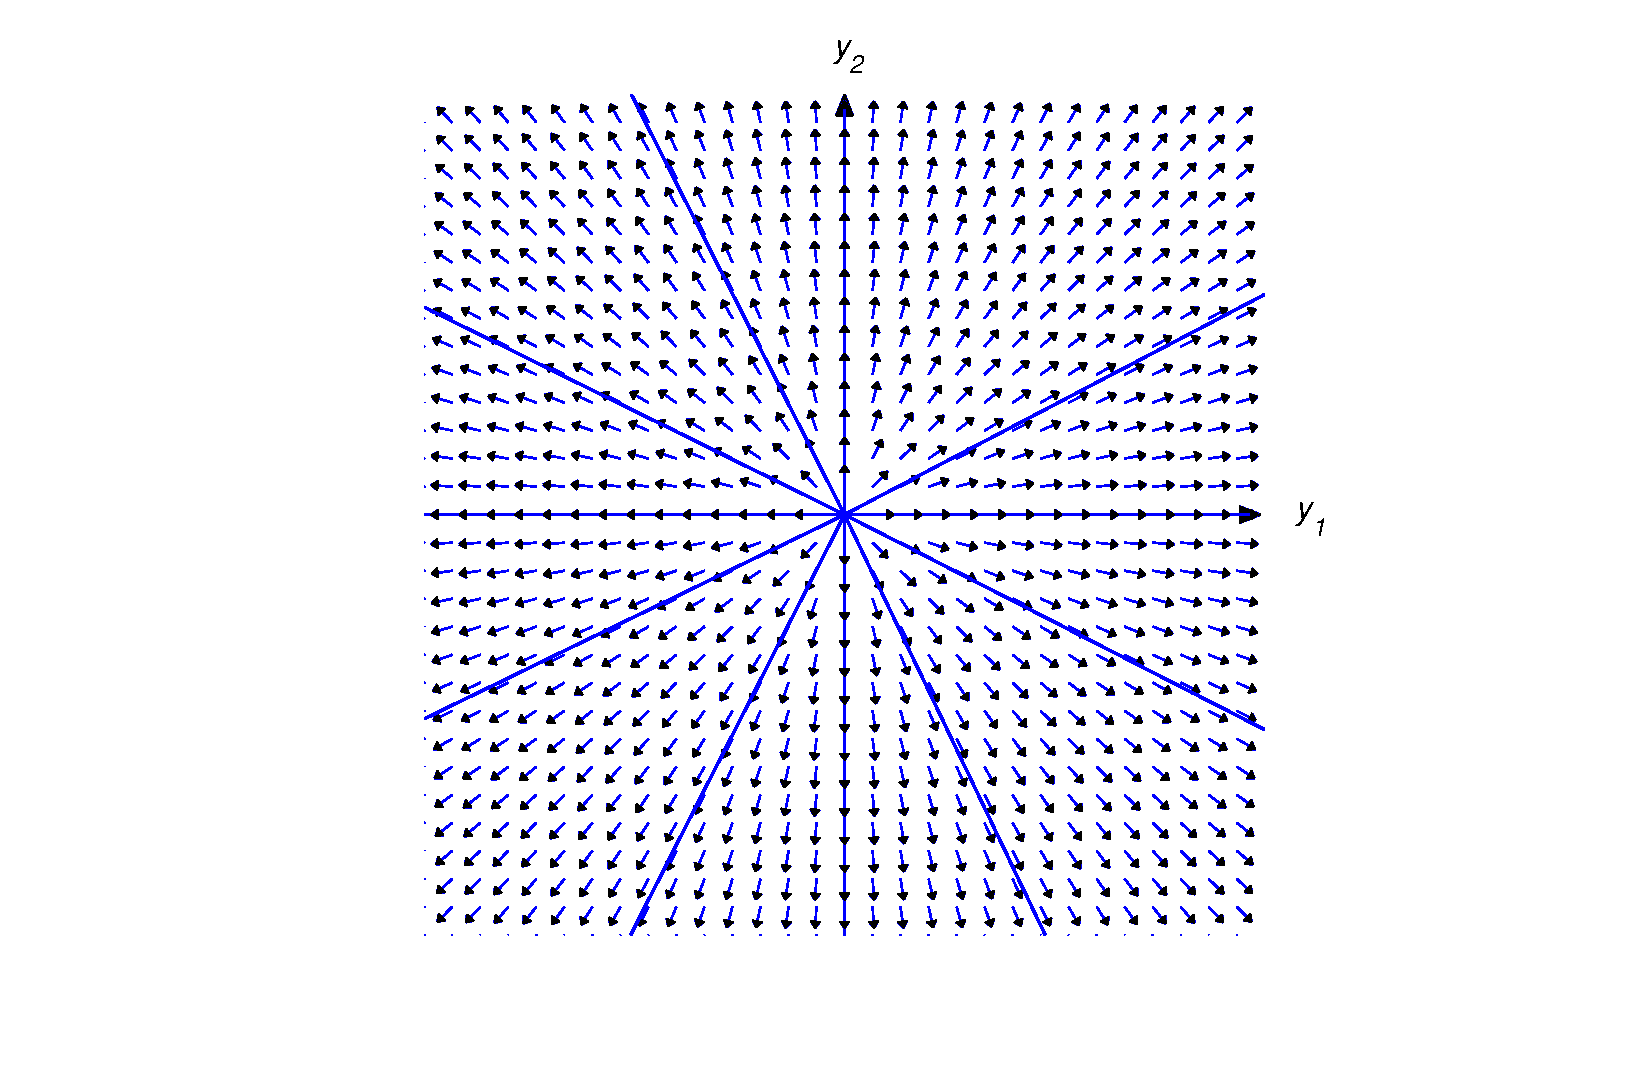
\includegraphics[bb=-78 148 689 643,width=5.67in,height=3.66in,keepaspectratio]{fig100401}}
\caption{
Trajectories of a $2\times2$ system with a repeated positive
eigenvalue}
  \label{figure:10.4.1}
\end{minipage}
  \begin{minipage}[b]{0.5\linewidth}
    \centering
   \scalebox{.65}{
  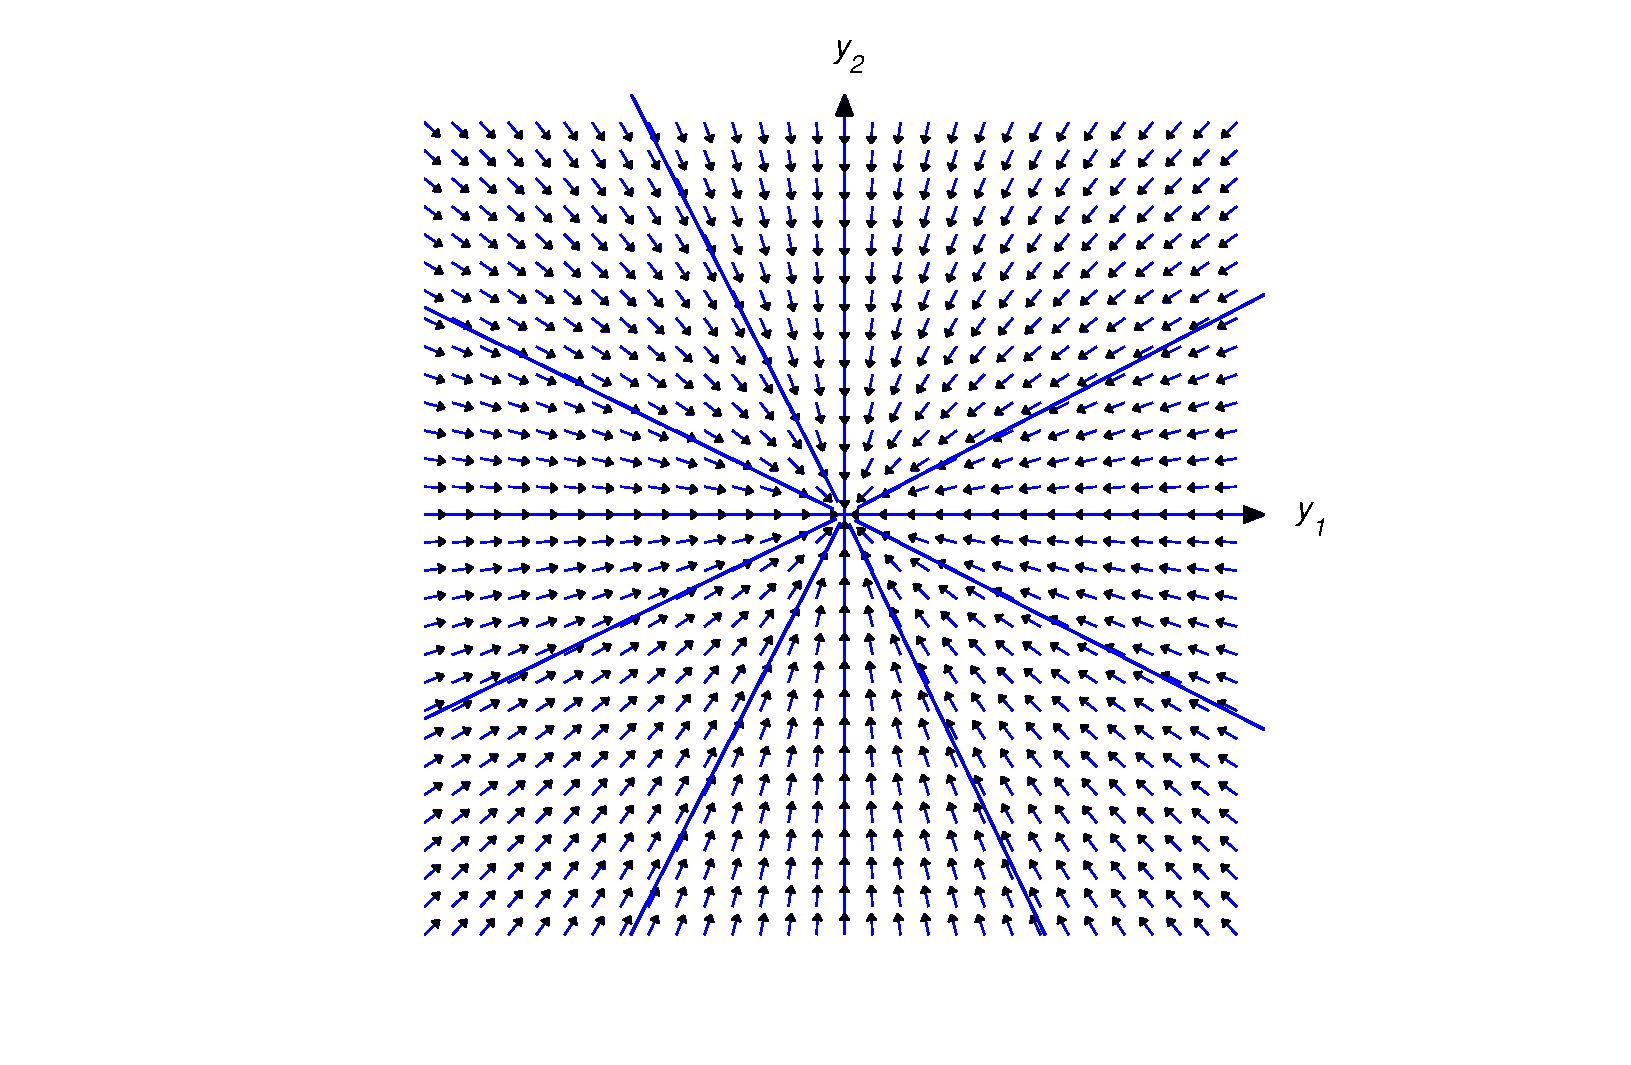
\includegraphics[bb=-78 148 689 643,width=5.67in,height=3.66in,keepaspectratio]{fig100402}}
\caption{
Trajectories of a $2\times2$ system with a repeated negative
eigenvalue}
  \label{figure:10.4.2}
\end{minipage}
\end{figure}

Now suppose   $\lambda_2>\lambda_1$, and let $L_1$ and $L_2$ denote
lines through the origin parallel to ${\bf x}_1$ and ${\bf x}_2$,
respectively. By a half-line of $L_1$ (or $L_2$), we mean either of the
rays obtained by removing the origin from $L_1$ (or $L_2$).

Letting $c_2=0$ in \eqref{eq:10.4.19} yields ${\bf y}=c_1{\bf
x}_1e^{\lambda_1 t}$. If $c_1\ne0$, the trajectory defined by this
solution is a half-line of $L_1$. The direction of motion is away from
the origin if $\lambda_1>0$, toward the origin if $\lambda_1<0$.
Similarly, the trajectory of  ${\bf y}=c_2{\bf x}_2e^{\lambda_2 t}$
with $c_2\ne0$ is a half-line of $L_2$.

Henceforth, we assume that $c_1$ and $c_2$ in \eqref{eq:10.4.19} are both
nonzero. In this case, the trajectory of \eqref{eq:10.4.19} can't
intersect
$L_1$ or $L_2$, since every point on these lines is on the trajectory
of a solution for which either $c_1=0$ or $c_2=0$. (Remember: distinct
trajectories can't intersect!). Therefore the trajectory of
\eqref{eq:10.4.19} must lie entirely in one of the four open sectors
bounded by $L_1$ and $L_2$, but do not any point  on $L_1$ or
$L_2$. Since the initial point $(y_1(0),y_2(0))$ defined by
$$
{\bf y}(0)=c_1{\bf x}_1+c_2{\bf x}_2
$$
is on the trajectory, we can determine which sector contains the
trajectory from the signs of $c_1$ and $c_2$,
as shown in Figure~\ref{figure:10.4.3}.

The direction of ${\bf y}(t)$ in \eqref{eq:10.4.19} is the
same as that of
\begin{equation} \label{eq:10.4.20}
e^{-\lambda_2 t}{\bf y}(t)=
c_1{\bf x}_1e^{-(\lambda_2-\lambda_1)t}+c_2{\bf x}_2
\end{equation}
and of
\begin{equation} \label{eq:10.4.21}
e^{-\lambda_1 t}{\bf y}(t)=c_1{\bf
x}_1+c_2{\bf x}_2e^{(\lambda_2-\lambda_1)t}.
\end{equation}
Since the right side of \eqref{eq:10.4.20} approaches $c_2{\bf x}_2$ as
$t\to\infty$, the trajectory is asymptotically parallel to $L_2$ as
$t\to\infty$. Since the right side of \eqref{eq:10.4.21} approaches
$c_1{\bf x}_1$ as $t\to-\infty$, the trajectory is asymptotically
parallel to $L_1$ as $t\to-\infty$.

The shape and direction of
traversal of the trajectory of \eqref{eq:10.4.19} depend upon whether
$\lambda_1$ and $\lambda_2$ are both positive, both negative, or of
opposite signs. We'll now analyze these three cases.

Henceforth $\|{\bf u}\|$  denote the length of the vector
${\bf u}$.

\begin{figure}[htbp]
\color{blue}
  \begin{minipage}[b]{0.5\linewidth}
    \centering
   \scalebox{.65}{
  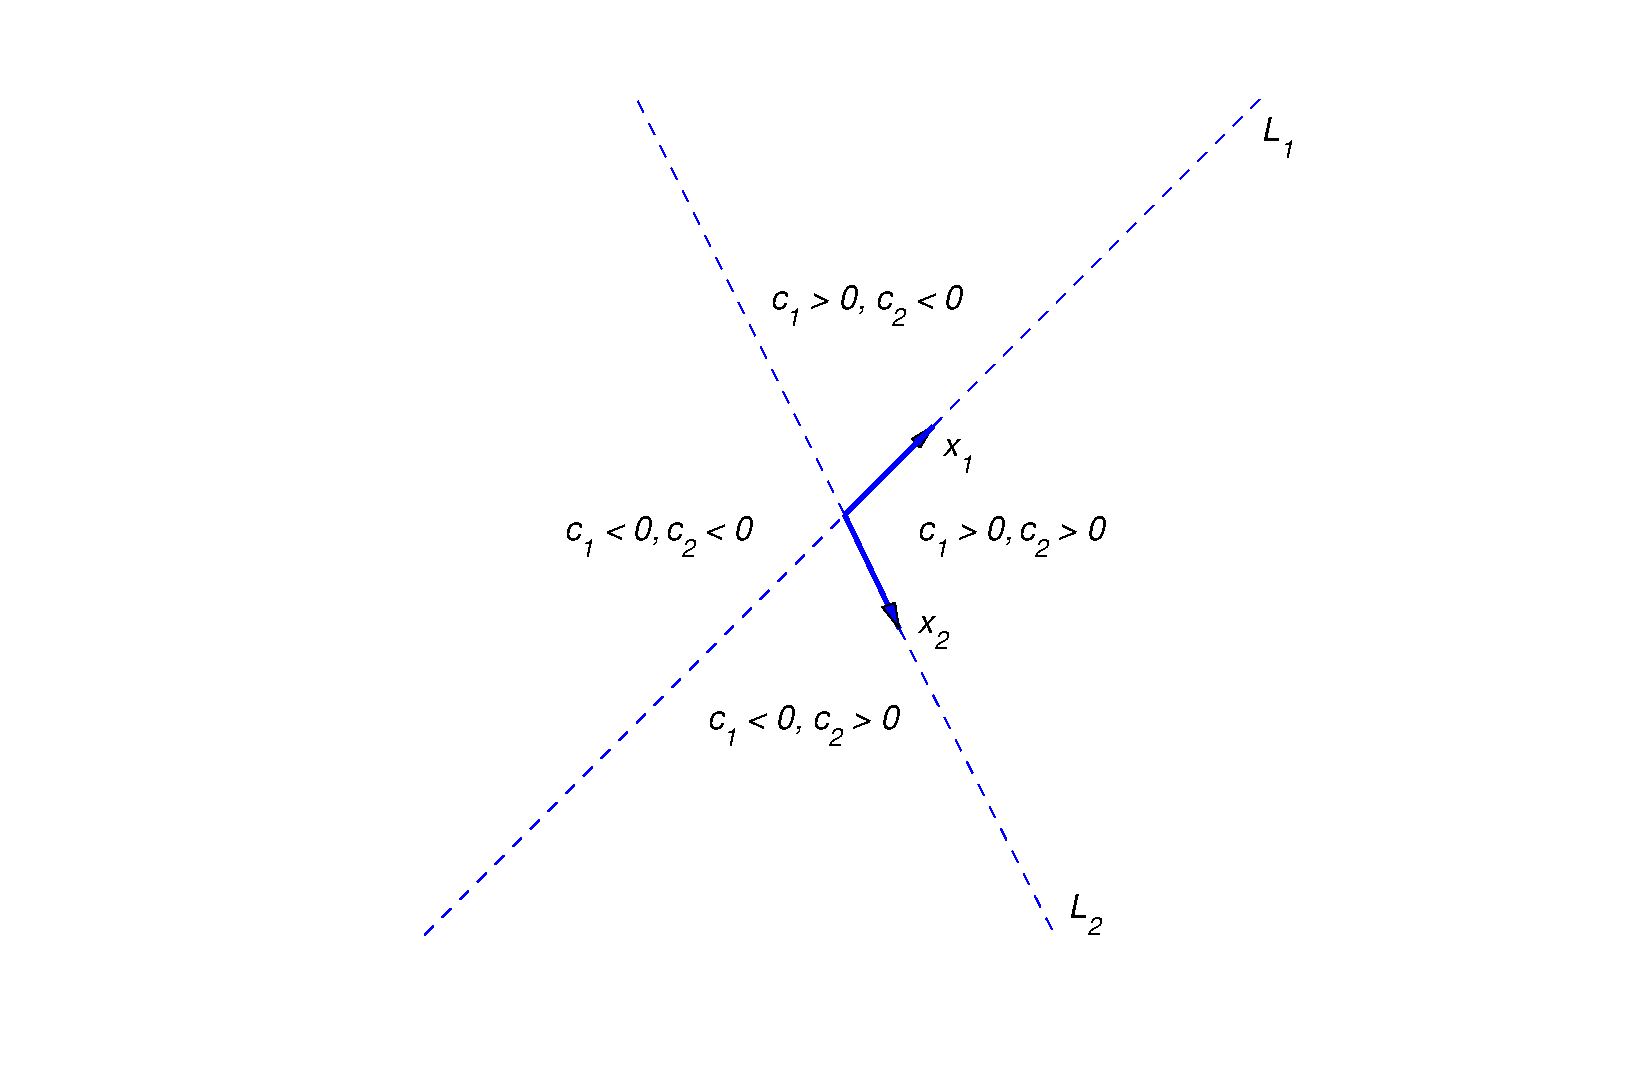
\includegraphics[bb=-78 148 689 643,width=5.67in,height=3.66in,keepaspectratio]{fig100403} }
  \caption{ Four open sectors bounded by $L_1$ and $L_2$}
  \label{figure:10.4.3}
\end{minipage}
  \begin{minipage}[b]{0.5\linewidth}
    \centering
   \scalebox{.65}{
  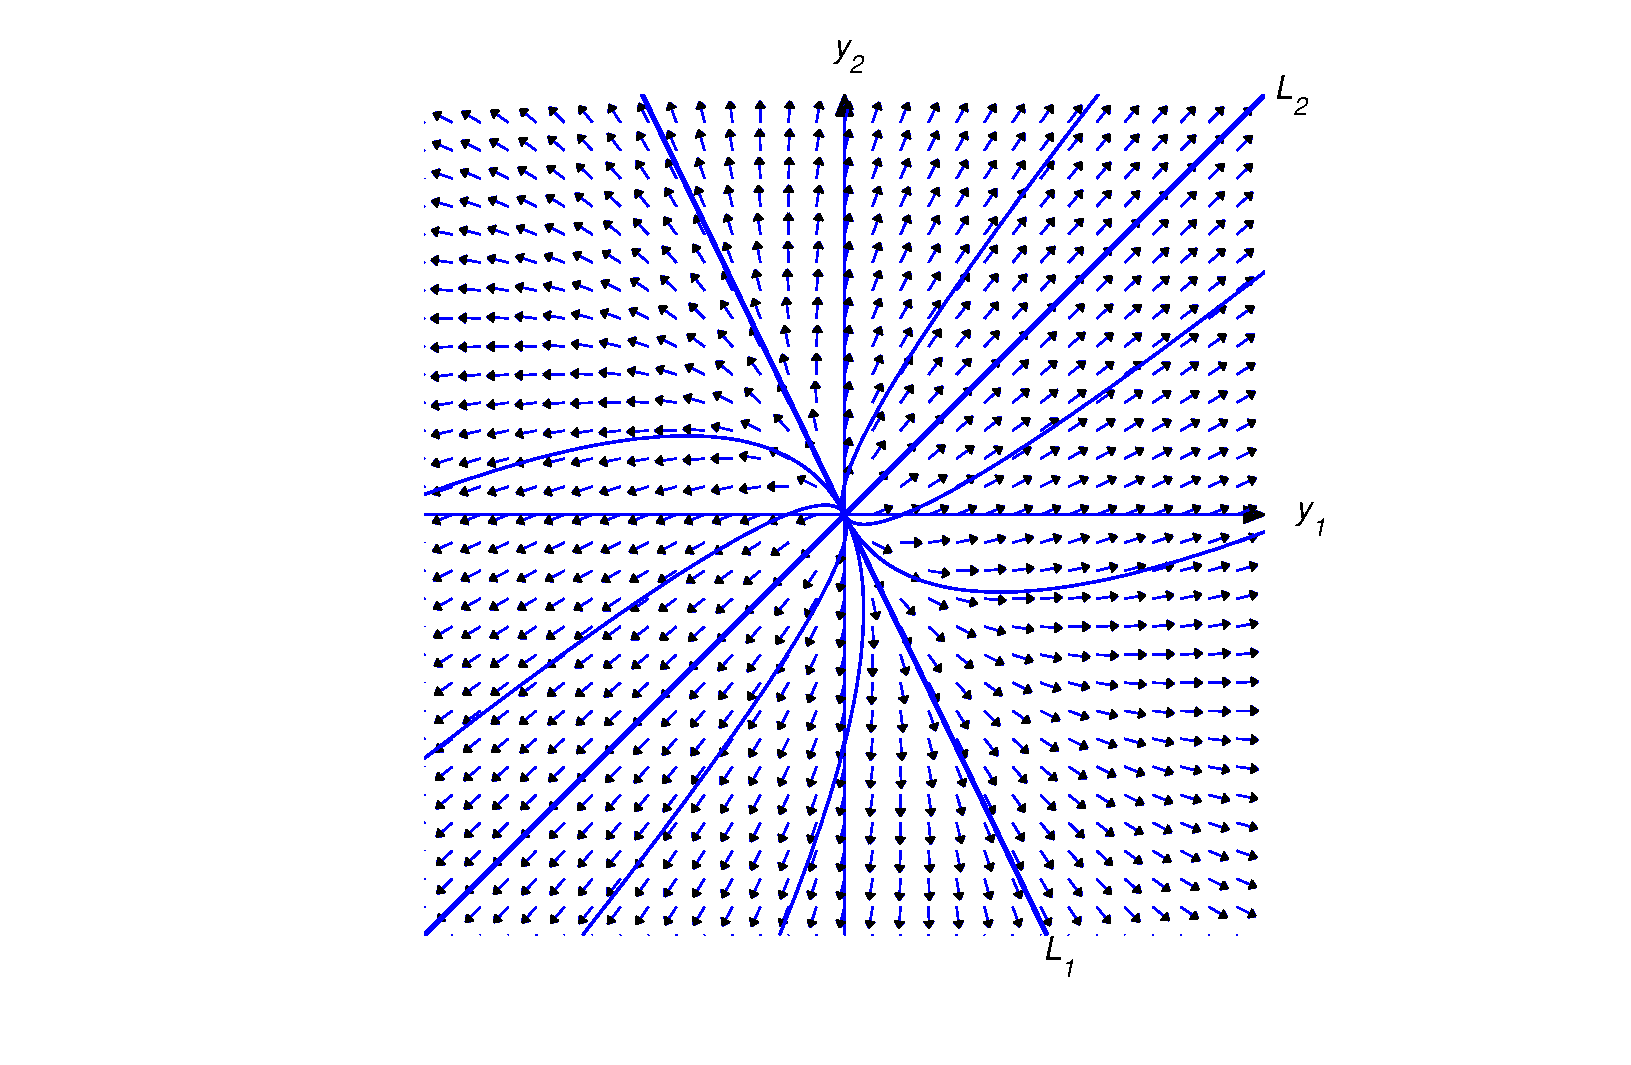
\includegraphics[bb=-78 148 689 643,width=5.67in,height=3.66in,keepaspectratio]{fig100404}  }
\caption{ Two positive eigenvalues;   motion away from
origin}
  \label{figure:10.4.4}
\end{minipage}
\end{figure}

\boxit{Case 1: $\lambda_2>\lambda_1>0$}

\noindent
Figure~\ref{figure:10.4.4}  shows some
 typical trajectories.
In this case, $\lim_{t\to-\infty}\|{\bf y}(t)\|=0$, so the trajectory
is not only asymptotically parallel to $L_1$ as $t\to-\infty$, but is
actually asymptotically tangent to $L_1$ at the origin. On
the other hand, $\lim_{t\to\infty}\|{\bf y}(t)\|=\infty$ and
$$
\lim_{t\to\infty}\left\|{\bf y}(t)-c_2{\bf x}_2e^{\lambda_2
t}\right\|=\lim_{t\to\infty}\|c_1{\bf x_1}e^{\lambda_1t}\|=\infty,
$$
so, although the trajectory is asymptotically parallel to $L_2$ as
$t\to\infty$, it's not asymptotically tangent to $L_2$.
The direction of motion along each trajectory is away from the origin.

\boxit{Case 2: $0>\lambda_2>\lambda_1$}

\noindent
Figure~\ref{figure:10.4.5}   shows
some typical trajectories.
In this case, $\lim_{t\to\infty}\|{\bf y}(t)\|=0$, so the trajectory is
asymptotically tangent to $L_2$ at the origin as $t\to\infty$. On the
other hand, $\lim_{t\to-\infty}\|{\bf y}(t)\|=\infty$ and
$$
\lim_{t\to-\infty}\left\|{\bf y}(t)-c_1{\bf x}_1e^{\lambda_1
t}\right\|=\lim_{t\to-\infty}\|c_2{\bf x}_2e^{\lambda_2t}\|=\infty,
$$
so, although the trajectory is asymptotically parallel to $L_1$ as
$t\to-\infty$, it's not asymptotically tangent to it.
The direction of motion along each trajectory is toward the origin.

\begin{figure}[htbp]
\color{blue}
  \begin{minipage}[b]{0.5\linewidth}
    \centering
   \scalebox{.65}{
  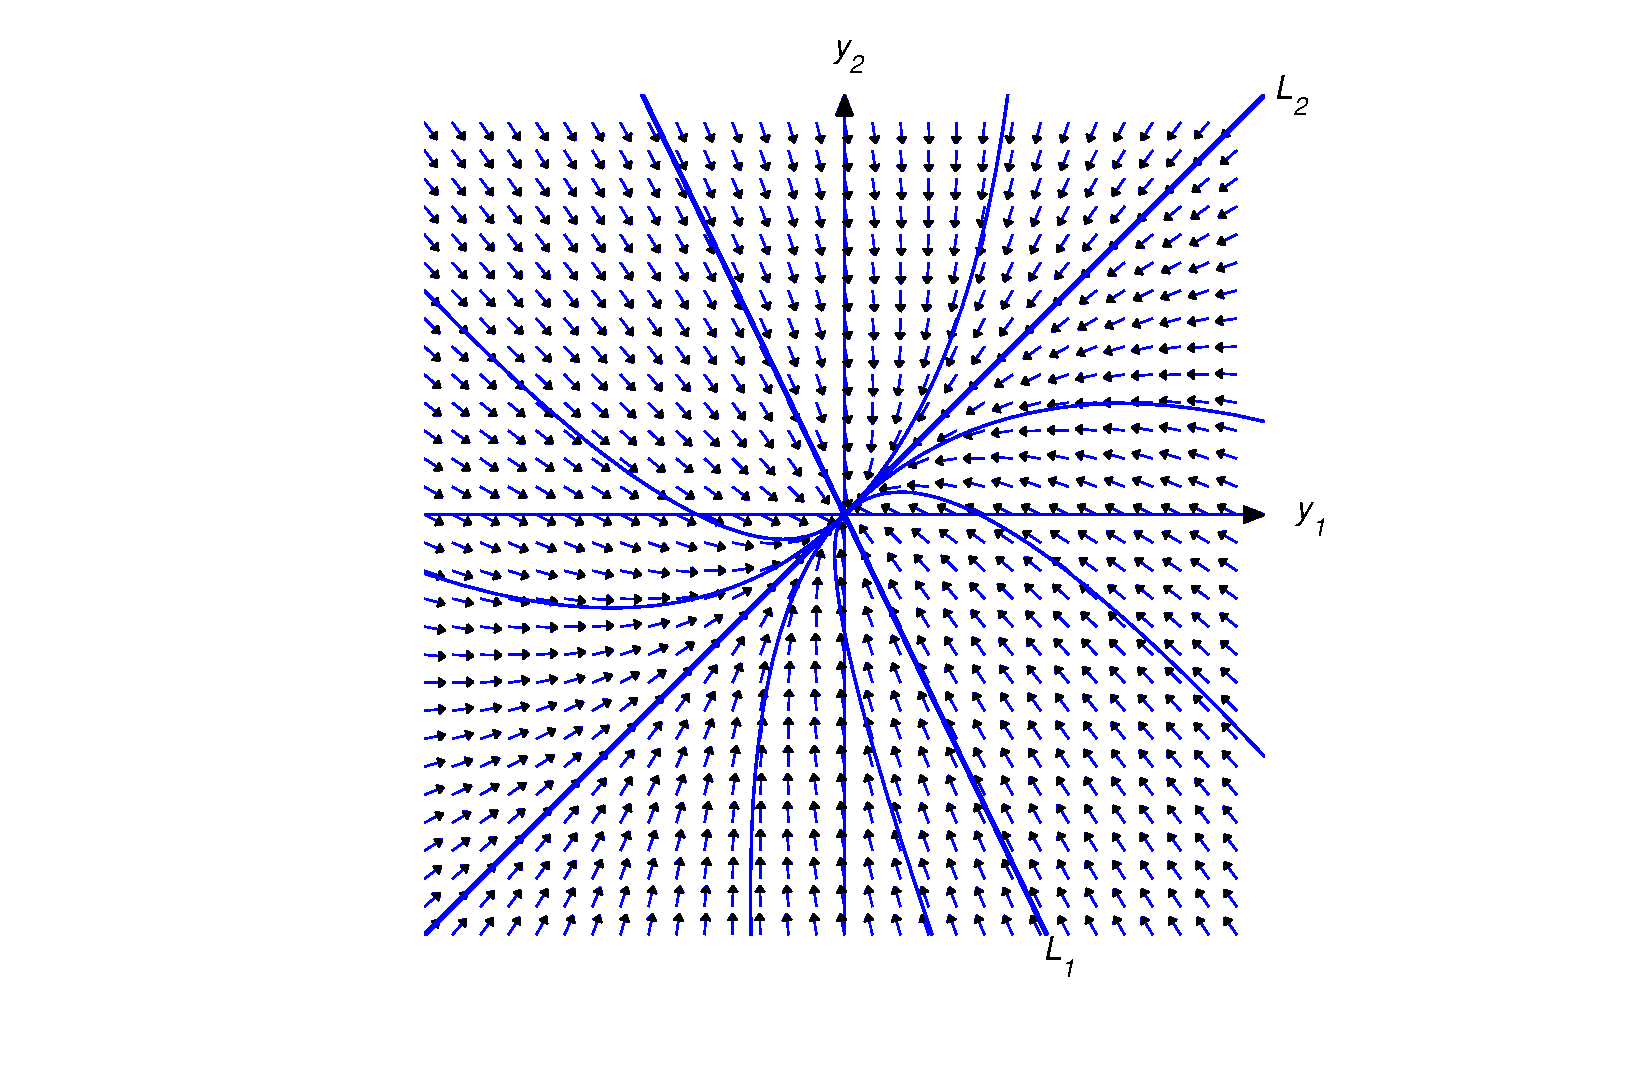
\includegraphics[bb=-78 148 689 643,width=5.67in,height=3.66in,keepaspectratio]{fig100405} }
\caption{
 Two negative eigenvalues;   motion toward the origin}
  \label{figure:10.4.5}
\end{minipage}
  \begin{minipage}[b]{0.5\linewidth}
    \centering
   \scalebox{.65}{
  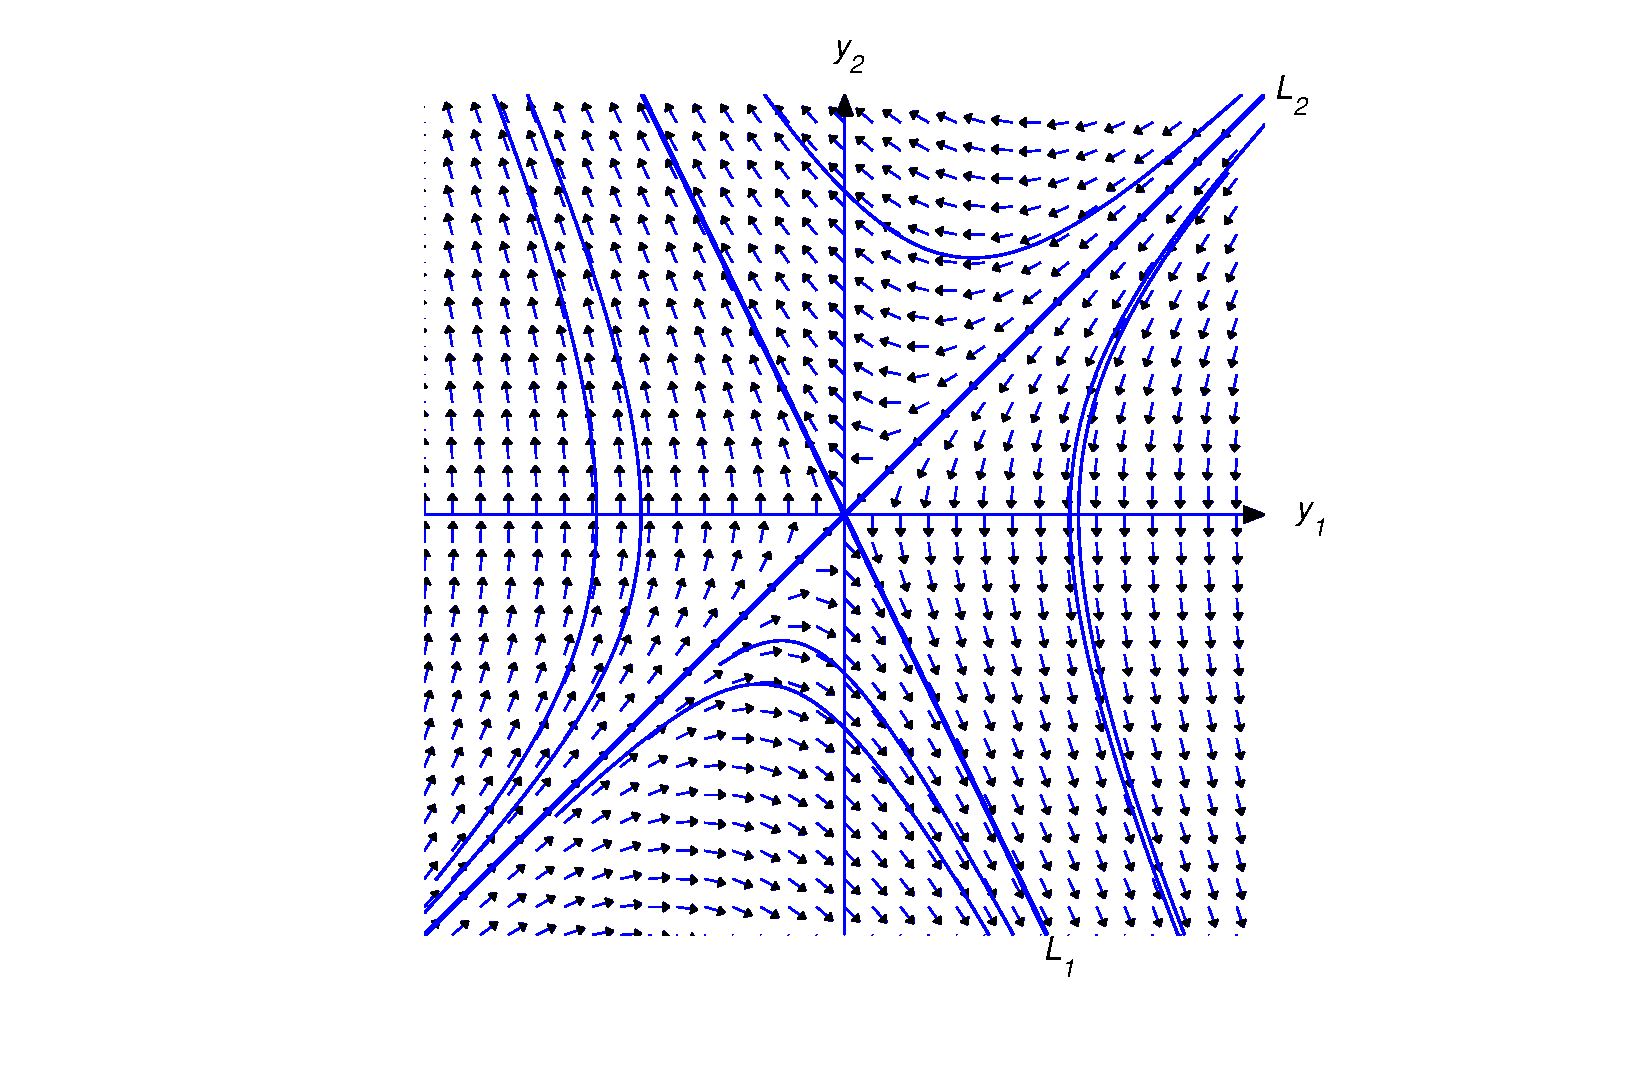
\includegraphics[bb=-78 148 689 643,width=5.67in,height=3.66in,keepaspectratio]{fig100406}}
\caption{ Eigenvalues of different signs}
  \label{figure:10.4.6}
\end{minipage}
\end{figure}

\boxit{Case 3: $\lambda_2>0>\lambda_1$}

\noindent
Figure~\ref{figure:10.4.6} shows
some typical trajectories.
In this case,
$$
\lim_{t\to\infty}\|{\bf y}(t)\|=\infty \mbox{\quad and \quad}
\lim_{t\to\infty}\left\|{\bf y}(t)-c_2{\bf x}_2e^{\lambda_2
t}\right\|=\lim_{t\to\infty}\|c_1{\bf x}_1e^{\lambda_1t}\|=0,
$$
so the trajectory is asymptotically tangent to $L_2$ as $t\to\infty$.
Similarly,
$$
\lim_{t\to-\infty}\|{\bf y}(t)\|=\infty \mbox{\quad and \quad}
\lim_{t\to-\infty}\left\|{\bf y}(t)-c_1{\bf x}_1e^{\lambda_1
t}\right\|=\lim_{t\to-\infty}\|c_2{\bf x}_2e^{\lambda_2t}\|=0,
$$
so the trajectory is asymptotically tangent to $L_1$ as $t\to-\infty$.
The direction of motion is toward the origin on $L_1$ and away from
the origin on $L_2$. The direction of motion along any other
trajectory is away from $L_1$, toward $L_2$.

\exercises
 In Exercises~\ref{exer:10.4.1}--\ref{exer:10.4.15} find the general
solution.

\begin{exerciselist}
\begin{tabular}[t]{@{}p{168pt}@{}p{168pt}}
\item\label{exer:10.4.1} $\dst{{\bf y}'=
\left[\begin{array}{rr} 1&2\\2&1\end{array}\right]{\bf y}}$&
\item\label{exer:10.4.2} $\dst{{\bf y}'=
{1\over4}\left[\begin{array}{rr}-5&3 \\3&-5\end{array}\right]{\bf
y}}$
\end{tabular}

\begin{tabular}[t]{@{}p{168pt}@{}p{168pt}}
\item\label{exer:10.4.3} $\dst{{\bf y}'=
{1\over5}\left[\begin{array}{rr}-4&3\\
-2&-11\end{array}\right]{\bf y}}$&
\item\label{exer:10.4.4} $\dst{{\bf y}'=
\left[\begin{array}{rr}-1&-4\\-1&-1\end{array}\right]{\bf y}}$
\end{tabular}

\begin{tabular}[t]{@{}p{168pt}@{}p{168pt}}
\item\label{exer:10.4.5} $\dst{{\bf y}'=
\left[\begin{array}{rr} 2&-4\\-1&-1\end{array}\right]{\bf y}}$&
\item\label{exer:10.4.6} $\dst{{\bf y}'=
\left[\begin{array}{rr} 4&-3\\2&-1\end{array}\right]{\bf y}}$
\end{tabular}

\begin{tabular}[t]{@{}p{168pt}@{}p{168pt}}
\item\label{exer:10.4.7} $\dst{{\bf y}'=
\left[\begin{array}{rr}-6&-3\\1&-2\end{array}\right]{\bf y}}$&
\item\label{exer:10.4.8} $\dst{{\bf y}'=
\left[\begin{array}{rrr}
1&-1&-2\\1&-2&-3\\-4&1&-1\end{array}\right]
{\bf y}}$
\end{tabular}

\begin{tabular}[t]{@{}p{168pt}@{}p{168pt}}
\item\label{exer:10.4.9} $\dst{{\bf y}'=
\left[\begin{array}{rrr}
-6&-4&-8\\-4&0&-4\\-8&-4&-6\end{array}\right]{\bf y}}$&
\item\label{exer:10.4.10} $\dst{{\bf y}'=
\left[\begin{array}{rrr}3&5&8\\1&-1&
-2\\-1&-1&-1\end{array}\right]{\bf y}}$
\end{tabular}

\begin{tabular}[t]{@{}p{168pt}@{}p{168pt}}
\item\label{exer:10.4.11}  $\dst{{\bf y}'=
\left[\begin{array}{rrr}
1&-1&2\\12&-4
& 10\\-6&1&-7
\end{array}\right]{\bf y}}$&
\item\label{exer:10.4.12} $\dst{{\bf y}'=
\left[\begin{array}{rrr}
4&-1&-4\\4&-3&-2\\1&-1&-1\end{array}\right]{\bf y}}$
\end{tabular}

\begin{tabular}[t]{@{}p{168pt}@{}p{168pt}}
\item\label{exer:10.4.13} $\dst{{\bf y}'=
\left[\begin{array}{rrr}-2&2&-6\\2&6&2\\-2&-2&
2\end{array}\right]{\bf y}}$&
\item\label{exer:10.4.14} $\dst{{\bf y}'=
\left[\begin{array}{rrr}3&2&-2\\-2&7&-2\\
-10&10&-5\end{array}\right]{\bf y}}$ \end{tabular}

\item\label{exer:10.4.15} $\dst{{\bf y}'=
\left[\begin{array}{rrr}3&1&-1\\3&5&1\\-6&2&4\end{array}
\right]{\bf y}}$

\exercisetext{In Exercises~\ref{exer:10.4.16}--\ref{exer:10.4.27}
solve the initial value problem.}

\item\label{exer:10.4.16}
$\dst{{\bf y}'=\twobytwo{-7}4{-6}7{\bf y},\quad{\bf
y}(0)=\twocol2{-4}}$

\item\label{exer:10.4.17}
$\dst{{\bf y}'={1\over6}\twobytwo72{-2}2{\bf y},\quad{\bf
y}(0)=\twocol0{-3}}$

\item\label{exer:10.4.18}
$\dst{{\bf y}'=\twobytwo{21}{-12}{24}{-15}{\bf y},\quad{\bf
y}(0)=\twocol53}$

\item\label{exer:10.4.19}
$\dst{{\bf y}'=\twobytwo{-7}4{-6}7{\bf y},\quad{\bf
y}(0)=\twocol{-1}7}$

\item\label{exer:10.4.20}
$\dst{{\bf y}'={1\over6}\threebythree1204{-1}0003{\bf y},\quad{\bf
y}(0)=\threecol471}$

\item\label{exer:10.4.21}
$\dst{{\bf y}'={1\over3}\threebythree2{-2}3{-4}43210{\bf
y},\quad{\bf y}(0)=\threecol115}$

\item\label{exer:10.4.22}
$\dst{{\bf y}'=\threebythree6{-3}{-8}21{-2}3{-3}{-5}{\bf
y},\quad{\bf y}(0)=\threecol0{-1}{-1}}$

\item\label{exer:10.4.23}
$\dst{{\bf y}'={1\over3}\threebythree24{-7}15{-5}{-4}4{-1}{\bf
y},\quad{\bf y}(0)=\threecol413}$

\item\label{exer:10.4.24} $\dst{
{\bf y}'=\threebythree301{11}{-2}7103{\bf y},\quad
{\bf y}(0)=\threecol276}$

\item\label{exer:10.4.25} $\dst{
{\bf y}'=\threebythree{-2}{-5}{-1}{-4}{-1}145{3}{\bf y},\quad
{\bf y}(0)=\threecol8{-10}{-4}}$

\item\label{exer:10.4.26}  $\dst{
{\bf y}'=\threebythree3{-1}04{-2}04{-4}2{\bf y},\quad
{\bf y}(0)=\threecol7{10}2}$

\item\label{exer:10.4.27} $\dst{{\bf y}'=
\left[\begin{array}{rrr}-2&2&6\\2&6&2\\-2&-2&
2\end{array}\right]{\bf y}},\quad{\bf y}(0)=\threecol6{-10}7$

\item\label{exer:10.4.28}
Let $A$ be an $n\times n$ constant matrix. Then
Theorem~\ref{thmtype:10.2.1} implies that the solutions
of
$$
{\bf y}'=A{\bf y}
\eqno{\rm(A)}
$$
are all defined on $(-\infty,\infty)$.
\begin{alist}
\item % (a)
Use Theorem~\ref{thmtype:10.2.1} to show that the only
solution
of (A) that can ever equal the zero vector is ${\bf y}\equiv{\bf0}$.
\item % (b)
Suppose ${\bf y}_1$ is a solution of (A) and ${\bf y}_2$ is
defined by ${\bf y}_2(t)={\bf y}_1(t-\tau)$, where $\tau$ is an
arbitrary real number. Show that ${\bf y}_2$ is also a solution of
(A).
\item % (c)
Suppose ${\bf y}_1$ and ${\bf y}_2$ are solutions of (A) and
there are real numbers $t_1$ and $t_2$ such that ${\bf y}_1(t_1)={\bf
y}_2(t_2)$. Show that ${\bf y}_2(t)={\bf y}_1(t-\tau)$ for all $t$,
where $\tau=t_2-t_1$. \hint{Show that ${\bf y}_1(t-\tau)$ and ${\bf
y}_2(t)$ are solutions of the same initial value problem for {\rm
(A)},
and apply the uniqueness assertion of
Theorem~\ref{thmtype:10.2.1}.}
\end{alist}

\exercisetext{In Exercises~\ref{exer:10.4.29}-~\ref{exer:10.4.34}
describe and graph trajectories of the given system.}

\begin{tabular}[t]{@{}p{168pt}@{}p{168pt}}
\item\label{exer:10.4.29} \CGex ${\bf y}'=\dst{\twobytwo111{-1}}{\bf y}$&
\item\label{exer:10.4.30} \CGex ${\bf y}'=\dst{\twobytwo{-4}3{-2}{-11}}{\bf
y}$
\end{tabular}

\begin{tabular}[t]{@{}p{168pt}@{}p{168pt}}
\item\label{exer:10.4.31} \CGex ${\bf y}'=\dst{\twobytwo9{-3}{-1}{11}}{\bf
y}$&
\item\label{exer:10.4.32} \CGex ${\bf
y}'=\dst{\twobytwo{-1}{-10}{-5}4}{\bf y}$
\end{tabular}

\begin{tabular}[t]{@{}p{168pt}@{}p{168pt}}
\item\label{exer:10.4.33} \CGex ${\bf y}'=\dst{\twobytwo5{-4}1{10}}{\bf
y}$&
\item\label{exer:10.4.34} \CGex ${\bf
y}'=\dst{\twobytwo{-7}13{-5}}{\bf y}$
\end{tabular}

\item\label{exer:10.4.35}
Suppose the eigenvalues of the $2\times 2$
matrix $A$ are $\lambda=0$ and $\mu\ne0$, with
corresponding  eigenvectors ${\bf x}_1$ and ${\bf x}_2$.
Let $L_1$ be the line through the origin parallel to ${\bf x}_1$.
\begin{alist}
\item % (a)
Show that every point on $L_1$ is the trajectory of a constant
solution of ${\bf y}'=A{\bf y}$.
\item % (b)
Show that the trajectories of nonconstant solutions of ${\bf y}'=A{\bf
y}$ are half-lines parallel to ${\bf x}_2$ and on either side of
$L_1$, and that the direction of motion along these trajectories is
away from $L_1$ if $\mu>0$, or toward $L_1$ if $\mu<0$.
\end{alist}

\exercisetext{The matrices of the systems in
Exercises~\ref{exer:10.4.36}-\ref{exer:10.4.41} are singular. Describe
and graph the trajectories of nonconstant solutions  of the given
systems.}

\begin{tabular}[t]{@{}p{168pt}@{}p{168pt}}
\item\label{exer:10.4.36} \CGex ${\bf y}'=\dst{\twobytwo{-1}11{-1}}{\bf y}$&
\item\label{exer:10.4.37} \CGex ${\bf y}'=\dst{\twobytwo{-1}{-3}26}{\bf
y}$
\end{tabular}

\begin{tabular}[t]{@{}p{168pt}@{}p{168pt}}
\item\label{exer:10.4.38} \CGex ${\bf y}'=\dst{\twobytwo1{-3}{-1}3}{\bf
y}$&
\item\label{exer:10.4.39} \CGex ${\bf y}'=\dst{\twobytwo1{-2}{-1}2}{\bf y}$
\end{tabular}

\begin{tabular}[t]{@{}p{168pt}@{}p{168pt}}
\item\label{exer:10.4.40} \CGex ${\bf y}'=\dst{\twobytwo{-4}{-4}11}{\bf
y}$&
\item\label{exer:10.4.41} \CGex ${\bf
y}'=\dst{\twobytwo3{-1}{-3}1}{\bf y}$
\end{tabular}

\item\label{exer:10.4.42} \Lex
Let $P=P(t)$ and $Q=Q(t)$ be the populations of two species at time
$t$, and assume that each population would grow exponentially if the
other didn't exist; that is, in the absence of competition,
$$
P'=aP \mbox{\quad and \quad}Q'=bQ,
\eqno{\rm(A)}
$$
where $a$ and $b$ are positive constants. One way to model the effect
of competition is to assume that the growth rate per individual of
each population is reduced by an amount proportional to the other
population, so (A) is replaced by
\begin{eqnarray*}
P'&=&\phantom{-}aP-\alpha Q\\
Q'&=&-\beta P+bQ,
\end{eqnarray*}
where $\alpha$ and $\beta$ are positive constants. (Since negative
population doesn't make sense, this system holds only while $P$ and
$Q$ are both positive.) Now suppose $P(0)=P_0>0$ and
$Q(0)=Q_0>0$.

\begin{alist}
\item % (a)
For several choices of $a$, $b$, $\alpha$, and $\beta$, verify
experimentally
(by graphing trajectories of (A) in the $P$-$Q$ plane) that there's a
constant $\rho>0$ (depending upon $a$, $b$, $\alpha$, and $\beta$) with the
following properties:
\begin{rmlist}
\item % (i)
If $Q_0>\rho P_0$, then $P$ decreases monotonically to zero
in finite time, during which $Q$ remains positive.
\item % (ii)
If $Q_0<\rho P_0$, then $Q$ decreases monotonically to zero in
finite time, during which $P$ remains positive.
\end{rmlist}
\item % (b)
Conclude from  \part{a} that exactly one of the species
becomes extinct in finite time if $Q_0\ne\rho P_0$. Determine
experimentally what happens if $Q_0=\rho P_0$.
\item % (c)
Confirm your experimental results and determine $\gamma$ by expressing
the eigenvalues and associated eigenvectors of
$$
A=\twobytwo a{-\alpha}{-\beta}b
$$
in terms of $a$, $b$, $\alpha$, and $\beta$, and applying the geometric
arguments developed at the end of this section.
\end{alist}

\end{exerciselist}


\section{Constant Coefficient Homogeneous Systems II}

\noindent
We saw in Section~10.4 that if an $n\times n$ constant matrix $A$ has $n$ real eigenvalues
$\lambda_{1}$, $\lambda_{2}$, \dots, $\lambda_{n}$ (which need not be distinct) with associated
linearly independent eigenvectors ${\bf x}_{1}$, ${\bf x}_{2}$, \dots, ${\bf x}_{n}$, then the
general solution of ${\bf y}'=A{\bf y}$ is
\[
  {\bf y}=c_{1}{\bf x}_{1}e^{\lambda_{1}t}+c_{2}{\bf x}_{2}e^{\lambda_{2}t}+\cdots+c_{n}{\bf x}_{n}e^{\lambda_{n}t}.
\]
In this section we consider the case where $A$ has $n$ real eigenvalues, but does not have $n$
linearly independent eigenvectors. It is shown in linear algebra that this occurs if and only if $A$
has at least one eigenvalue of multiplicity $r>1$ such that the associated eigenspace has dimension
less than $r$. In this case $A$ is said to be {\color{blue}\it defective\/}. Since it's beyond the
scope of this book to give a complete analysis of systems with defective coefficient matrices, we
will restrict our attention to some commonly occurring special cases.

\begin{example}
  \label{example:10.5.1}\rm \space Show that the system
  \begin{equation}
    \label{eq:10.5.1}{\bf y}'=\twobytwo{11}{-25}4{-9}{\bf y}
  \end{equation}
  does not have a fundamental set of solutions of the form
  $\{{\bf x}_{1}e^{\lambda_{1}t},{\bf x}_{2}e^{\lambda_{2}t}\}$, where $\lambda_{1}$ and
  $\lambda_{2}$ are eigenvalues of the coefficient matrix $A$ of \eqref{eq:10.5.1} and
  ${\bf x}_{1}$ and ${\bf x}_{2}$ are associated linearly independent eigenvectors.
\end{example}

\solution The characteristic polynomial of $A$ is
\begin{eqnarray*}
  \twochar{11}{-25}4{-9} & = & (\lambda-11)(\lambda+9)+100 \\
                         & = & \lambda^{2}-2\lambda+1=(\lambda-1)^{2}.
\end{eqnarray*}
Hence, $\lambda=1$ is the only eigenvalue of $A$. The augmented matrix of the system
$(A-I){\bf x}={\bf0}$ is
\[
  \left[
  \begin{array}{rrcr}
    10 & -25 & \vdots & 0 \\
    4  & -10 & \vdots & 0
  \end{array}\right],
\]
which is row equivalent to
\[
  \left[
  \begin{array}{rrcr}
    1 & -\dst\frac{5}{2} & \vdots & 0 \\[10pt]
    0 & 0                & \vdots & 0
  \end{array}\right].
\]
Hence, $x_{1}=5x_{2}/2$ where $x_{2}$ is arbitrary. Therefore all eigenvectors of $A$ are scalar
multiples of ${\bf x}_{1}=\dst{\twocol52}$, so $A$ does not have a set of two linearly independent
eigenvectors. \bbox

From Example~\ref{example:10.5.1}, we know that all scalar multiples of
${\bf y}_{1}=\dst{\twocol52}e^{t}$ are solutions of \eqref{eq:10.5.1}; however, to find the general
solution we must find a second solution ${\bf y}_{2}$ such that $\{{\bf y}_{1},{\bf y}_{2}\}$ is
linearly independent. Based on your recollection of the procedure for solving a constant coefficient
scalar equation
\[
  ay''+by'+cy=0
\]
in the case where the characteristic polynomial has a repeated root, you might expect to obtain a
second solution of \eqref{eq:10.5.1} by multiplying the first solution by $t$. However, this yields
${\bf y}_{2}=\dst{\twocol52}te^{t}$, which doesn't work, since
\[
  {\bf y}_{2}'=\twocol52(te^{t}+e^{t}),\mbox{\quad while \quad }\twobytwo{11}{-25}4{-9}{\bf y}_{2}=\twocol52te^{t}.
\]

The next theorem shows what to do in this situation.

\begin{theorem}
  \color{blue}
  \label{thmtype:10.5.1} Suppose the $n\times n$ matrix $A$ has an eigenvalue $\lambda_{1}$ of
  multiplicity $\ge2$ and the associated eigenspace has dimension $1$; that is, all
  $\lambda_{1}$-eigenvectors of $A$ are scalar multiples of an eigenvector ${\bf x}$. Then there are
  infinitely many vectors ${\bf u}$ such that
  \begin{equation}
    \label{eq:10.5.2}(A-\lambda_{1}I){\bf u}={\bf x}.
  \end{equation}
  Moreover, if ${\bf u}$ is any such vector then
  \begin{equation}
    \label{eq:10.5.3}{\bf y}_{1}={\bf x}e^{\lambda_{1}t}\quad\mbox{and }\quad{\bf y}_{2}={\bf u}e^{\lambda_{1}t}+{\bf x}te^{\lambda_{1}t}
  \end{equation}
  are linearly independent solutions of ${\bf y}'=A{\bf y}$.
\end{theorem}

A complete proof of this theorem is beyond the scope of this book. The difficulty is in proving that
there's a vector ${\bf u}$ satisfying \eqref{eq:10.5.2}, since $\det(A-\lambda_{1}I)=0$. We'll take
this without proof and verify the other assertions of the theorem.

We already know that ${\bf y}_{1}$ in \eqref{eq:10.5.3} is a solution of ${\bf y}'=A{\bf y}$. To see
that ${\bf y}_{2}$ is also a solution, we compute
\begin{eqnarray*}
  {\bf y}_{2}'-A{\bf y}_{2} & = & \lambda_{1}{\bf u}e^{\lambda_{1}t}+{\bf x}e^{\lambda_{1}t}+\lambda_{1}{\bf x}te^{\lambda_{1}t}-A{\bf u}e^{\lambda_{1}t}-A{\bf x}te^{\lambda_{1}t} \\
                            & = & (\lambda_{1}{\bf u}+{\bf x}-A{\bf u})e^{\lambda_{1}t}+(\lambda_{1}{\bf x}-A{\bf x})te^{\lambda_{1}t}.
\end{eqnarray*}
Since $A{\bf x}=\lambda_{1}{\bf x}$, this can be written as
\[
  {\bf y}_{2}'-A{\bf y}_{2}=- \left((A-\lambda_{1}I){\bf u}-{\bf x}\right)e^{\lambda_{1}t},
\]
and now \eqref{eq:10.5.2} implies that ${\bf y}_{2}'=A{\bf y}_{2}$.

To see that ${\bf y}_{1}$ and ${\bf y}_{2}$ are linearly independent, suppose $c_{1}$ and $c_{2}$
are constants such that
\begin{equation}
  \label{eq:10.5.4}c_{1}{\bf y}_{1}+c_{2}{\bf y}_{2}=c_{1}{\bf x}e^{\lambda_{1}t}+c_{2}({\bf u}e^{\lambda_{1}t}+{\bf x}te^{\lambda_{1}t})={\bf0}.
\end{equation}
We must show that $c_{1}=c_{2}=0$. Multiplying \eqref{eq:10.5.4} by $e^{-\lambda_{1}t}$ shows that
\begin{equation}
  \label{eq:10.5.5}c_{1}{\bf x}+c_{2}({\bf u}+{\bf x}t)={\bf0}.
\end{equation}
By differentiating this with respect to $t$, we see that $c_{2}{\bf x}={\bf0}$, which implies
$c_{2}=0$, because ${\bf x}\ne{\bf0}$. Substituting $c_{2}=0$ into \eqref{eq:10.5.5} yields
$c_{1}{\bf x}={\bf0}$, which implies that $c_{1}=0$, again because ${\bf x}\ne{\bf0}$.
\begin{example}
  \label{example:10.5.2}\rm Use Theorem~\ref{thmtype:10.5.1} to find the general solution of the
  system
  \begin{equation}
    \label{eq:10.5.6}{\bf y}'=\twobytwo{11}{-25}4{-9}{\bf y}
  \end{equation}
  considered in Example~\ref{example:10.5.1}.
\end{example}

\solution In Example~\ref{example:10.5.1} we saw that $\lambda_{1}=1$ is an eigenvalue of
multiplicity $2$ of the coefficient matrix $A$ in \eqref{eq:10.5.6}, and that all of the
eigenvectors of $A$ are multiples of
\[
  {\bf x}=\twocol52.
\]
Therefore
\[
  {\bf y}_{1}=\twocol52e^{t}
\]
is a solution of \eqref{eq:10.5.6}. From Theorem~\ref{thmtype:10.5.1}, a second solution is given by
${\bf y}_{2}={\bf u}e^{t}+{\bf x}te^{t}$, where $(A-I){\bf u}={\bf x}$. The augmented matrix of this
system is
\[
  \left[
  \begin{array}{rrcr}
    10 & -25 & \vdots & 5 \\
    4  & -10 & \vdots & 2
  \end{array}\right],
\]
which is row equivalent to
\[
  \dst{\left[\begin{array}{rrcr}1&-\frac{5}{2}&\vdots&1\over2\\ 0&0&\vdots&0\end{array}\right]}.
\]
Therefore the components of ${\bf u}$ must satisfy
\[
  u_{1}-\frac{5}{2}u_{2}=\frac{1}{2},
\]
where $u_{2}$ is arbitrary. We choose $u_{2}=0$, so that $u_{1}=1/2$ and
\[
  {\bf u}=\twocol{\frac{1}{2}}0.
\]
Thus,
\[
  {\bf y}_{2}=\twocol10{\frac{e^{t}}{2}}+\twocol52te^{t}.
\]
Since ${\bf y}_{1}$ and ${\bf y}_{2}$ are linearly independent by Theorem~\ref{thmtype:10.5.1}, they
form a fundamental set of solutions of \eqref{eq:10.5.6}. Therefore the general solution of
\eqref{eq:10.5.6} is
\[
  {\bf y}=c_{1}\twocol52e^{t}+c_{2}\left(\twocol10{\frac{e^{t}}{2}}+\twocol52te^{t}\right).\bbox
\]

Note that choosing the arbitrary constant $u_{2}$ to be nonzero is equivalent to adding a scalar
multiple of ${\bf y}_{1}$ to the second solution ${\bf y}_{2}$ (Exercise~\ref{exer:10.5.33}).

\begin{example}
  \label{example:10.5.3}\rm Find the general solution of
  \begin{equation}
    \label{eq:10.5.7}{\bf y}'=\threebythree34{-10}21{-2}22{-5}{\bf y}.
  \end{equation}
\end{example}

\solution The characteristic polynomial of the coefficient matrix $A$ in \eqref{eq:10.5.7} is
\[
  \left|
  \begin{array}{ccc}
    3-\lambda & 4         & -10        \\
    2         & 1-\lambda & -2         \\
    2         & 2         & -5-\lambda
  \end{array}\right|=- (\lambda-1)(\lambda+1)^{2}.
\]
Hence, the eigenvalues are $\lambda_{1}=1$ with multiplicity~$1$ and $\lambda_{2}=-1$ with
multiplicity~$2$.

Eigenvectors associated with $\lambda_{1}=1$ must satisfy $(A-I){\bf x}={\bf0}$. The augmented
matrix of this system is
\[
  \left[
  \begin{array}{rrrcr}
    2 & 4 & -10 & \vdots & 0 \\
    2 & 0 & -2  & \vdots & 0 \\
    2 & 2 & -6  & \vdots & 0
  \end{array}\right],
\]
which is row equivalent to
\[
  \left[
  \begin{array}{rrrcr}
    1 & 0 & -1 & \vdots & 0 \\
    0 & 1 & -2 & \vdots & 0 \\
    0 & 0 & 0  & \vdots & 0
  \end{array}\right].
\]
Hence, $x_{1}=x_{3}$ and $x_{2}=2x_{3}$, where $x_{3}$ is arbitrary. Choosing $x_{3}=1$ yields the
eigenvector
\[
  {\bf x}_{1}=\threecol121.
\]
Therefore
\[
  {\bf y}_{1}=\threecol121e^{t}
\]
is a solution of \eqref{eq:10.5.7}.

Eigenvectors associated with $\lambda_{2}=-1$ satisfy $(A+I){\bf x}={\bf0}$. The augmented matrix of
this system is
\[
  \left[
  \begin{array}{rrrcr}
    4 & 4 & -10 & \vdots & 0 \\
    2 & 2 & -2  & \vdots & 0 \\
    2 & 2 & -4  & \vdots & 0
  \end{array}\right],
\]
which is row equivalent to
\[
  \left[
  \begin{array}{rrrcr}
    1 & 1 & 0 & \vdots & 0 \\
    0 & 0 & 1 & \vdots & 0 \\
    0 & 0 & 0 & \vdots & 0
  \end{array}\right].
\]
Hence, $x_{3}=0$ and $x_{1}=-x_{2}$, where $x_{2}$ is arbitrary. Choosing $x_{2}=1$ yields the
eigenvector
\[
  {\bf x}_{2}=\threecol{-1}10,
\]
so
\[
  {\bf y}_{2}=\threecol{-1}10e^{-t}
\]
is a solution of \eqref{eq:10.5.7}.

Since all the eigenvectors of $A$ associated with $\lambda_{2}=-1$ are multiples of ${\bf x}_{2}$,
we must now use Theorem~\ref{thmtype:10.5.1} to find a third solution of \eqref{eq:10.5.7} in the
form
\begin{equation}
  \label{eq:10.5.8}{\bf y}_{3}={\bf u}e^{-t}+\threecol{-1}10te^{-t},
\end{equation}
where ${\bf u}$ is a solution of $(A+I){\bf u}={\bf x}_{2}$. The augmented matrix of this system is
\[
  \left[
  \begin{array}{rrrcr}
    4 & 4 & -10 & \vdots & -1 \\
    2 & 2 & -2  & \vdots & 1  \\
    2 & 2 & -4  & \vdots & 0
  \end{array}\right],
\]
which is row equivalent to
\[
  \left[
  \begin{array}{rrrcr}
    1 & 1 & 0 & \vdots & 1           \\
    0 & 0 & 1 & \vdots & \frac{1}{2} \\
    0 & 0 & 0 & \vdots & 0
  \end{array}\right].
\]
Hence, $u_{3}=1/2$ and $u_{1}=1-u_{2}$, where $u_{2}$ is arbitrary. Choosing $u_{2}=0$ yields
\[
  {\bf u}=\threecol10{\frac{1}{2}},
\]
and substituting this into \eqref{eq:10.5.8} yields the solution
\[
  {\bf y}_{3}=\threecol201{\frac{e^{-t}}{2}}+\threecol{-1}10te^{-t}
\]
of \eqref{eq:10.5.7}.

Since the Wronskian of $\{{\bf y}_{1},{\bf y}_{2},{\bf y}_{3}\}$ at $t=0$ is
\[
  \left|
  \begin{array}{rrr}
    1 & -1 & 1       \\
    2 & 1  & 0       \\
    1 & 0  & 1\over2
  \end{array}\right|=\frac{1}{2},
\]
$\{{\bf y}_{1},{\bf y}_{2},{\bf y}_{3}\}$ is a fundamental set of solutions of \eqref{eq:10.5.7}.
Therefore the general solution of \eqref{eq:10.5.7} is
\[
  {\bf y}=c_{1}\threecol121e^{t}+c_{2}\threecol{-1}10e^{-t}+c_{3}\left (\threecol201{\frac{e^{-t}}{2}}+\threecol{-1}10te^{-t}\right).
\]

\begin{theorem}
  \color{blue}
  \label{thmtype:10.5.2} Suppose the $n\times n$ matrix $A$ has an eigenvalue $\lambda_{1}$ of
  multiplicity $\ge3$ and the associated eigenspace is one--dimensional; that is, all eigenvectors
  associated with $\lambda_{1}$ are scalar multiples of the eigenvector ${\bf x}$. Then there are
  infinitely many vectors ${\bf u}$ such that
  \begin{equation}
    \label{eq:10.5.9}(A-\lambda_{1}I){\bf u}={\bf x},
  \end{equation}
  and, if ${\bf u}$ is any such vector, there are infinitely many vectors ${\bf v}$ such that
  \begin{equation}
    \label{eq:10.5.10}(A-\lambda_{1}I){\bf v}={\bf u}.
  \end{equation}
  If ${\bf u}$ satisfies {\rm\eqref{eq:10.5.9}} and ${\bf v}$ satisfies {\rm\eqref{eq:10.5.10}},
  then
  \begin{eqnarray*}
    {\bf y}_{1} & = & {\bf x}e^{\lambda_{1}t},                                      \\
    {\bf y}_{2} & = & {\bf u}e^{\lambda_{1}t}+{\bf x}te^{\lambda_{1}t},\mbox{ and } \\
    {\bf y}_{3} & = & {\bf v}e^{\lambda_{1}t}+{\bf u}te^{\lambda_{1}t}+{\bf x}{\frac{t^{2}e^{\lambda_{1}t}}{2}}
  \end{eqnarray*}
  are linearly independent solutions of ${\bf y}'=A{\bf y}$.
\end{theorem}

Again, it's beyond the scope of this book to prove that there are vectors ${\bf u}$ and ${\bf v}$
that satisfy \eqref{eq:10.5.9} and \eqref{eq:10.5.10}. Theorem~\ref{thmtype:10.5.1} implies that
${\bf y}_{1}$ and ${\bf y}_{2}$ are solutions of ${\bf y}'=A{\bf y}$. We leave the rest of the proof
to you (Exercise~\ref{exer:10.5.34}).

\begin{example}
  \label{example:10.5.4}\rm Use Theorem~\ref{thmtype:10.5.2} to find the general solution of
  \begin{equation}
    \label{eq:10.5.11}{\bf y}'=\threebythree11113{-1}022{\bf y}.
  \end{equation}
\end{example}

\solution The characteristic polynomial of the coefficient matrix $A$ in \eqref{eq:10.5.11} is
\[
  \left|
  \begin{array}{ccc}
    1-\lambda & 1         & \phantom{-}1 \\
    1         & 3-\lambda & -1           \\
    0         & 2         & 2-\lambda
  \end{array}\right|=-(\lambda-2)^{3}.
\]
Hence, $\lambda_{1}=2$ is an eigenvalue of multiplicity $3$. The associated eigenvectors satisfy
$(A-2I){\bf x}={\bf0}$. The augmented matrix of this system is
\[
  \left[
  \begin{array}{rrrcr}
    -1 & 1 & 1  & \vdots & 0 \\
    1  & 1 & -1 & \vdots & 0 \\
    0  & 2 & 0  & \vdots & 0
  \end{array}\right],
\]
which is row equivalent to
\[
  \left[
  \begin{array}{rrrcr}
    1 & 0 & -1 & \vdots & 0 \\
    0 & 1 & 0  & \vdots & 0 \\
    0 & 0 & 0  & \vdots & 0
  \end{array}\right].
\]
Hence, $x_{1}=x_{3}$ and $x_{2}=0$, so the eigenvectors are all scalar multiples of
\[
  {\bf x}_{1}=\threecol101.
\]
Therefore
\[
  {\bf y}_{1}=\threecol101e^{2t}
\]
is a solution of \eqref{eq:10.5.11}.

We now find a second solution of \eqref{eq:10.5.11} in the form
\[
  {\bf y}_{2}={\bf u}e^{2t}+\threecol101te^{2t},
\]
where ${\bf u}$ satisfies $(A-2I){\bf u}={\bf x}_{1}$. The augmented matrix of this system is
\[
  \left[
  \begin{array}{rrrcr}
    -1 & 1 & 1  & \vdots & 1 \\
    1  & 1 & -1 & \vdots & 0 \\
    0  & 2 & 0  & \vdots & 1
  \end{array}\right],
\]
which is row equivalent to
\[
  \left[
  \begin{array}{rrrcr}
    1 & 0 & -1 & \vdots & -\frac{1}{2} \\
    0 & 1 & 0  & \vdots & \frac{1}{2}  \\
    0 & 0 & 0  & \vdots & 0
  \end{array}\right].
\]
Letting $u_{3}=0$ yields $u_{1}=-1/2$ and $u_{2}=1/2$; hence,
\[
  {\bf u}=\frac{1}{2}\threecol{-1}10
\]
and
\[
  {\bf y}_{2}=\threecol{-1}10{\frac{e^{2t}}{2}}+\threecol101te^{2t}
\]
is a solution of \eqref{eq:10.5.11}.

We now find a third solution of \eqref{eq:10.5.11} in the form
\[
  {\bf y}_{3}={\bf v}e^{2t}+\threecol{-1}10{\frac{te^{2t}}{2}}+\threecol101{\frac{t^{2}e^{2t}}{2}}
\]
where ${\bf v}$ satisfies $(A-2I){\bf v}={\bf u}$. The augmented matrix of this system is
\[
  \left[
  \begin{array}{rrrcr}
    -1 & 1 & 1  & \vdots & -\frac{1}{2} \\
    1  & 1 & -1 & \vdots & \frac{1}{2}  \\
    0  & 2 & 0  & \vdots & 0
  \end{array}\right],
\]
which is row equivalent to
\[
  \left[
  \begin{array}{rrrcr}
    1 & 0 & -1 & \vdots & \frac{1}{2} \\
    0 & 1 & 0  & \vdots & 0           \\
    0 & 0 & 0  & \vdots & 0
  \end{array}\right].
\]
Letting $v_{3}=0$ yields $v_{1}=1/2$ and $v_{2}=0$; hence,
\[
  {\bf v}=\frac{1}{2}\threecol100.
\]
Therefore
\[
  {\bf y}_{3}=\threecol100{\frac{e^{2t}}{2}}+ \threecol{-1}10{\frac{te^{2t}}{2}}+\threecol101{\frac{t^{2}e^{2t}}{2}}
\]
is a solution of \eqref{eq:10.5.11}. Since ${\bf y}_{1}$, ${\bf y}_{2}$, and ${\bf y}_{3}$ are
linearly independent by Theorem~\ref{thmtype:10.5.2}, they form a fundamental set of solutions of
\eqref{eq:10.5.11}. Therefore the general solution of \eqref{eq:10.5.11} is
\begin{eqnarray*}
  {\bf y} & = & \dst{c_{1}\threecol101e^{2t}+c_{2}\left(\threecol{-1}10{\frac{e^{2t}}{2}}+\threecol101te^{2t}\right)} \\[2\jot]
          &   & +c_{3}\dst{\left(\threecol100{\frac{e^{2t}}{2}}+\threecol{-1}10{\frac{te^{2t}}{2}}+\threecol101{\frac{t^{2}e^{2t}}{2}}\right)}.
\end{eqnarray*}

\enlargethispage{1in}

\begin{theorem}
  \color{blue}
  \label{thmtype:10.5.3} Suppose the $n\times n$ matrix $A$ has an eigenvalue $\lambda_{1}$ of
  multiplicity $\ge3$ and the associated eigenspace is two--dimensional; that is, all eigenvectors
  of $A$ associated with $\lambda_{1}$ are linear combinations of two linearly independent
  eigenvectors ${\bf x}_{1}$ and ${\bf x}_{2}$. Then there are constants $\alpha$ and $\beta$ (not
  both zero) such that if
  \begin{equation}
    \label{eq:10.5.12}{\bf x}_{3}=\alpha{\bf x}_{1}+\beta{\bf x}_{2},
  \end{equation}
  then there are infinitely many vectors ${\bf u}$ such that
  \begin{equation}
    \label{eq:10.5.13}(A-\lambda_{1}I){\bf u}={\bf x}_{3}.
  \end{equation}
  If ${\bf u}$ satisfies {\rm\eqref{eq:10.5.13}}, then
  \begin{eqnarray}
    {\bf y}_{1} & = & {\bf x}_{1}e^{\lambda_{1}t},\nonumber            \\
    {\bf y}_{2} & = & {\bf x}_{2}e^{\lambda_{1}t},\mbox{and }\nonumber \\
    {\bf y}_{3} & = & {\bf u}e^{\lambda_{1}t}+{\bf x}_{3}te^{\lambda_{1}t}\label{eq:10.5.14},
  \end{eqnarray}
  are linearly independent solutions of ${\bf y}'=A{\bf y}$.
\end{theorem}

We omit the proof of this theorem.

\newpage

\begin{example}
  \label{example:10.5.5}\rm Use Theorem~\ref{thmtype:10.5.3} to find the general solution of
  \begin{equation}
    \label{eq:10.5.15}{\bf y}'=\threebythree001{-1}11{-1}02{\bf y}.
  \end{equation}
\end{example}

\solution The characteristic polynomial of the coefficient matrix $A$ in \eqref{eq:10.5.15} is
\[
  \left|
  \begin{array}{ccc}
    -\lambda & 0         & 1         \\
    -1       & 1-\lambda & 1         \\
    -1       & 0         & 2-\lambda
  \end{array}\right|=-(\lambda-1)^{3}.
\]
Hence, $\lambda_{1}=1$ is an eigenvalue of multiplicity $3$. The associated eigenvectors satisfy
$(A-I){\bf x}={\bf 0}$. The augmented matrix of this system is
\[
  \left[
  \begin{array}{rrrcr}
    -1 & 0 & 1 & \vdots & 0 \\
    -1 & 0 & 1 & \vdots & 0 \\
    -1 & 0 & 1 & \vdots & 0
  \end{array}\right],
\]
which is row equivalent to
\[
  \left[
  \begin{array}{rrrcr}
    1 & 0 & -1 & \vdots & 0 \\
    0 & 0 & 0  & \vdots & 0 \\
    0 & 0 & 0  & \vdots & 0
  \end{array}\right].
\]
Hence, $x_{1}=x_{3}$ and $x_{2}$ is arbitrary, so the eigenvectors are of the form
\[
  {\bf x}=\threecol{x_{3}}{x_{2}}{x_{3}}=x_{3}\threecol101+x_{2}\threecol010.
\]
Therefore the vectors
\begin{equation}
  \label{eq:10.5.16}{\bf x}_{1}=\threecol101\quad\mbox{and }\quad{\bf x}_{2}=\threecol010
\end{equation}
form a basis for the eigenspace, and
\[
  {\bf y}_{1}=\threecol101e^{t}\quad\mbox{and }\quad{\bf y}_{2}=\threecol010e^{t}
\]
are linearly independent solutions of \eqref{eq:10.5.15}.

To find a third linearly independent solution of \eqref{eq:10.5.15}, we must find constants $\alpha$
and $\beta$ (not both zero) such that the system
\begin{equation}
  \label{eq:10.5.17}(A-I){\bf u}=\alpha{\bf x}_{1}+\beta{\bf x}_{2}
\end{equation}
has a solution ${\bf u}$. The augmented matrix of this system is
\[
  \left[
  \begin{array}{rrrcr}
    -1 & 0 & 1 & \vdots & \alpha \\
    -1 & 0 & 1 & \vdots & \beta  \\
    -1 & 0 & 1 & \vdots & \alpha
  \end{array}\right],
\]
which is row equivalent to
\begin{equation}
  \label{eq:10.5.18}\left[
  \begin{array}{rrrcr}
    1 & 0 & -1 & \vdots & -\alpha      \\
    0 & 0 & 0  & \vdots & \beta-\alpha \\
    0 & 0 & 0  & \vdots & 0
  \end{array}
  \right].
\end{equation}
Therefore \eqref{eq:10.5.17} has a solution if and only if $\beta=\alpha$, where $\alpha$ is
arbitrary. If $\alpha=\beta=1$ then \eqref{eq:10.5.12} and \eqref{eq:10.5.16} yield
\[
  {\bf x}_{3}={\bf x}_{1}+{\bf x}_{2}= \threecol101+\threecol010=\threecol111,
\]
and the augmented matrix \eqref{eq:10.5.18} becomes
\[
  \left[
  \begin{array}{rrrcr}
    1 & 0 & -1 & \vdots & -1 \\
    0 & 0 & 0  & \vdots & 0  \\
    0 & 0 & 0  & \vdots & 0
  \end{array}
  \right].
\]
This implies that $u_{1}=-1+u_{3}$, while $u_{2}$ and $u_{3}$ are arbitrary. Choosing
$u_{2}=u_{3}=0$ yields
\[
  {\bf u}=\threecol{-1}00.
\]
Therefore \eqref{eq:10.5.14} implies that
\[
  {\bf y}_{3}={\bf u}e^{t}+{\bf x}_{3}te^{t}=\threecol{-1}00e^{t}+\threecol111te^{t}
\]
is a solution of \eqref{eq:10.5.15}. Since ${\bf y}_{1}$, ${\bf y}_{2}$, and ${\bf y}_{3}$ are
linearly independent by Theorem~\ref{thmtype:10.5.3}, they form a fundamental set of solutions for
\eqref{eq:10.5.15}. Therefore the general solution of \eqref{eq:10.5.15} is
\[
  {\bf y}=c_{1}\threecol101e^{t}+c_{2}\threecol010e^{t}+c_{3}\left(\threecol{-1}00e^{t}+\threecol111te^{t}\right).\bbox
\]

\boxit{Geometric Properties of Solutions when $n=2$}

\noindent
We'll now consider the geometric properties of solutions of a $2\times2$ constant coefficient system
\begin{equation}
  \label{eq:10.5.19}\twocol{y_{1}'}{y_{2}'}=\left[
  \begin{array}{cc}
    a_{11} & a_{12} \\
    a_{21} & a_{22}
  \end{array}\right]\twocol{y_{1}}{y_{2}}
\end{equation}
under the assumptions of this section; that is, when the matrix
\[
  A=\left[
  \begin{array}{cc}
    a_{11} & a_{12} \\
    a_{21} & a_{22}
  \end{array}\right]
\]
has a repeated eigenvalue $\lambda_{1}$ and the associated eigenspace is one-dimensional. In this
case we know from Theorem~\ref{thmtype:10.5.1} that the general solution of \eqref{eq:10.5.19} is
\begin{equation}
  \label{eq:10.5.20}{\bf y}=c_{1}{\bf x}e^{\lambda_{1}t}+c_{2}({\bf u}e^{\lambda_{1}t}+{\bf x}te^{\lambda_{1}t}),
\end{equation}
where ${\bf x}$ is an eigenvector of $A$ and ${\bf u}$ is any one of the infinitely many solutions
of
\begin{equation}
  \label{eq:10.5.21}(A-\lambda_{1}I){\bf u}={\bf x}.
\end{equation}
We assume that $\lambda_{1}\ne0$.

\begin{figure}[H]
  \centering
  \scalebox{.8}{
  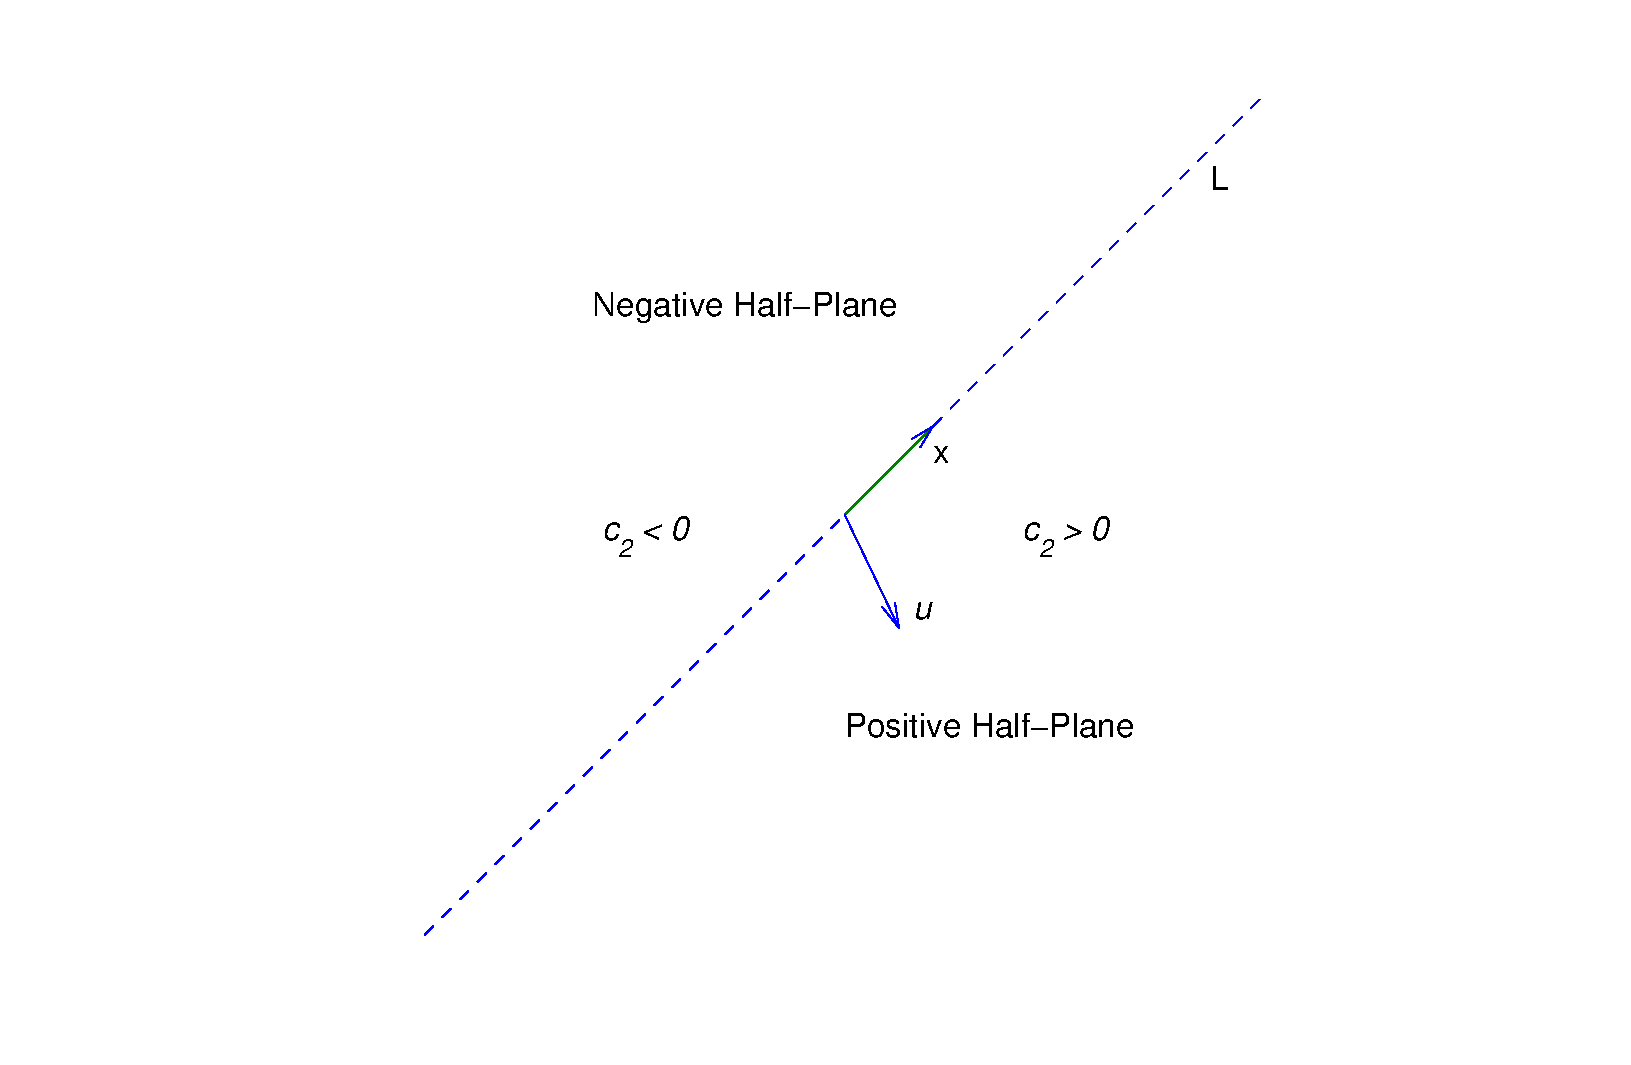
\includegraphics[bb=-78 148 689 643, width=5.67in, height=3.66in, keepaspectratio]{fig100501}}
  \caption{Positive and negative half-planes}
  \label{figure:10.5.1}
\end{figure}

Let $L$ denote the line through the origin parallel to ${\bf x}$. By a {\color{blue}\it half-line\/}
of $L$ we mean either of the rays obtained by removing the origin from $L$. Eqn.~\eqref{eq:10.5.20}
is a parametric equation of the half-line of $L$ in the direction of ${\bf x}$ if $c_{1}>0$, or of
the half-line of $L$ in the direction of $-{\bf x}$ if $c_{1}<0$. The origin is the trajectory of
the trivial solution ${\bf y}\equiv{\bf0}$.

Henceforth, we assume that $c_{2}\ne0$. In this case, the trajectory of \eqref{eq:10.5.20} can't
intersect $L$, since every point of $L$ is on a trajectory obtained by setting $c_{2}=0$. Therefore
the trajectory of \eqref{eq:10.5.20} must lie entirely in one of the open half-planes bounded by
$L$, but does not contain any point on $L$. Since the initial point $(y_{1}(0),y_{2}(0))$ defined by
${\bf y}(0)=c_{1}{\bf x}+c_{2}{\bf u}$ is on the trajectory, we can determine which half-plane
contains the trajectory from the sign of $c_{2}$, as shown in Figure~\ref{figure:10.5.1}. For
convenience we'll call the half-plane where $c_{2}>0$ the {\color{blue}\it positive half-plane\/}.
Similarly, the half- plane where $c_{2}<0$ is the {\color{blue}\it negative half-plane\/}. You should
convince yourself (Exercise~\ref{exer:10.5.35}) that even though there are infinitely many vectors
${\bf u}$ that satisfy \eqref{eq:10.5.21}, they all define the same positive and negative
half-planes. In the figures simply regard ${\bf u}$ as an arrow pointing to the positive half-plane,
since we haven't attempted to give ${\bf u}$ its proper length or direction in comparison with
${\bf x}$. For our purposes here, only the relative orientation of ${\bf x}$ and ${\bf u}$ is
important; that is, whether the positive half-plane is to the right of an observer facing the
direction of ${\bf x}$ (as in Figures~\ref{figure:10.5.2} and \ref{figure:10.5.5}), or to the left
of the observer (as in Figures~\ref{figure:10.5.3} and \ref{figure:10.5.4}).

Multiplying \eqref{eq:10.5.20} by $e^{-\lambda_{1}t}$ yields
\[
  e^{-\lambda_{1}t}{\bf y}(t)=c_{1}{\bf x}+c_{2}{\bf u}+c_{2}t{\bf x}.
\]
Since the last term on the right is dominant when $|t|$ is large, this provides the following
information on the direction of ${\bf y}(t)$:
\begin{alist}
  \item % (a)
  Along trajectories in the positive half-plane ($c_{2}>0$), the direction of ${\bf y}(t)$
  approaches the direction of ${\bf x}$ as $t\to\infty$ and the direction of $-{\bf x}$ as
  $t\to-\infty$.

  \item % (b)
  Along trajectories in the negative half-plane ($c_{2}<0$), the direction of ${\bf y}(t)$
  approaches the direction of $-{\bf x}$ as $t\to\infty$ and the direction of ${\bf x}$ as
  $t\to-\infty$.
\end{alist}

Since
\[
  \lim_{t\to\infty}\|{\bf y}(t)\|=\infty\mbox{\quad and \quad}\lim_{t\to-\infty}{\bf y}(t)={\bf0}\mbox{\quad if \quad}\lambda_{1}>0,
\]
or
\[
  \lim_{t\to-\infty}\|{\bf y}(t)\|=\infty\mbox{\quad and \quad}\lim_{t\to\infty}{\bf y}(t)={\bf0}\mbox{\quad if \quad}\lambda_{1}<0,
\]
there are four possible patterns for the trajectories of \eqref{eq:10.5.19}, depending upon the
signs of $c_{2}$ and $\lambda_{1}$. Figures~\ref{figure:10.5.2}-\ref{figure:10.5.5} illustrate these
patterns, and reveal the following principle:

{\color{blue}\it If $\lambda_{1}$ and $c_{2}$ have the same sign then the direction of the trajectory
approaches the direction of $-{\bf x}$ as $\|{\bf y}\|\to0$ and the direction of ${\bf x}$ as
$\|{\bf y}\|\to\infty$. If $\lambda_{1}$ and $c_{2}$ have opposite signs then the direction of the
trajectory approaches the direction of ${\bf x}$ as $\|{\bf y}\|\to0$ and the direction of
$-{\bf x}$ as $\|{\bf y}\|\to\infty$.}

\begin{figure}[H]
  \color{blue}
  \begin{minipage}[b]{0.5\linewidth}
    \centering
    \scalebox{.65}{
    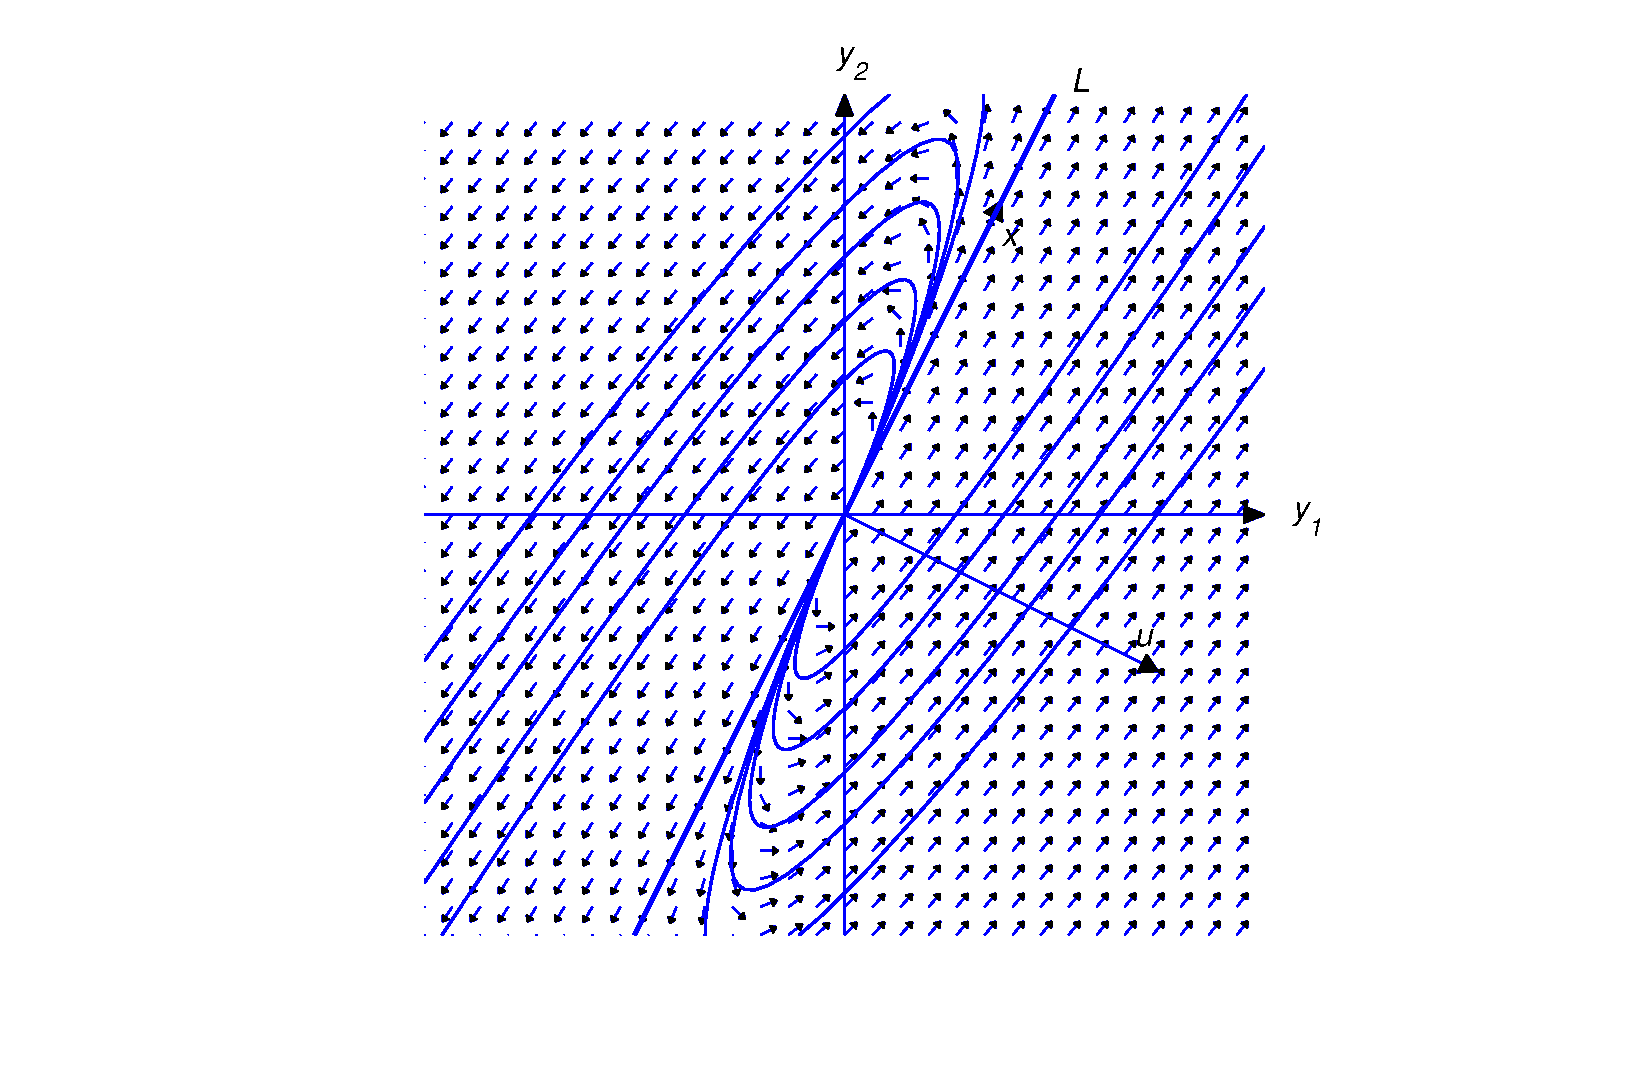
\includegraphics[bb=-78 148 689 643, width=5.67in, height=3.66in, keepaspectratio]{fig100502}}
    \caption{Positive eigenvalue; motion away from the origin}
    \label{figure:10.5.2}
  \end{minipage}
  \begin{minipage}[b]{0.5\linewidth}
    \centering
    \scalebox{.65}{
    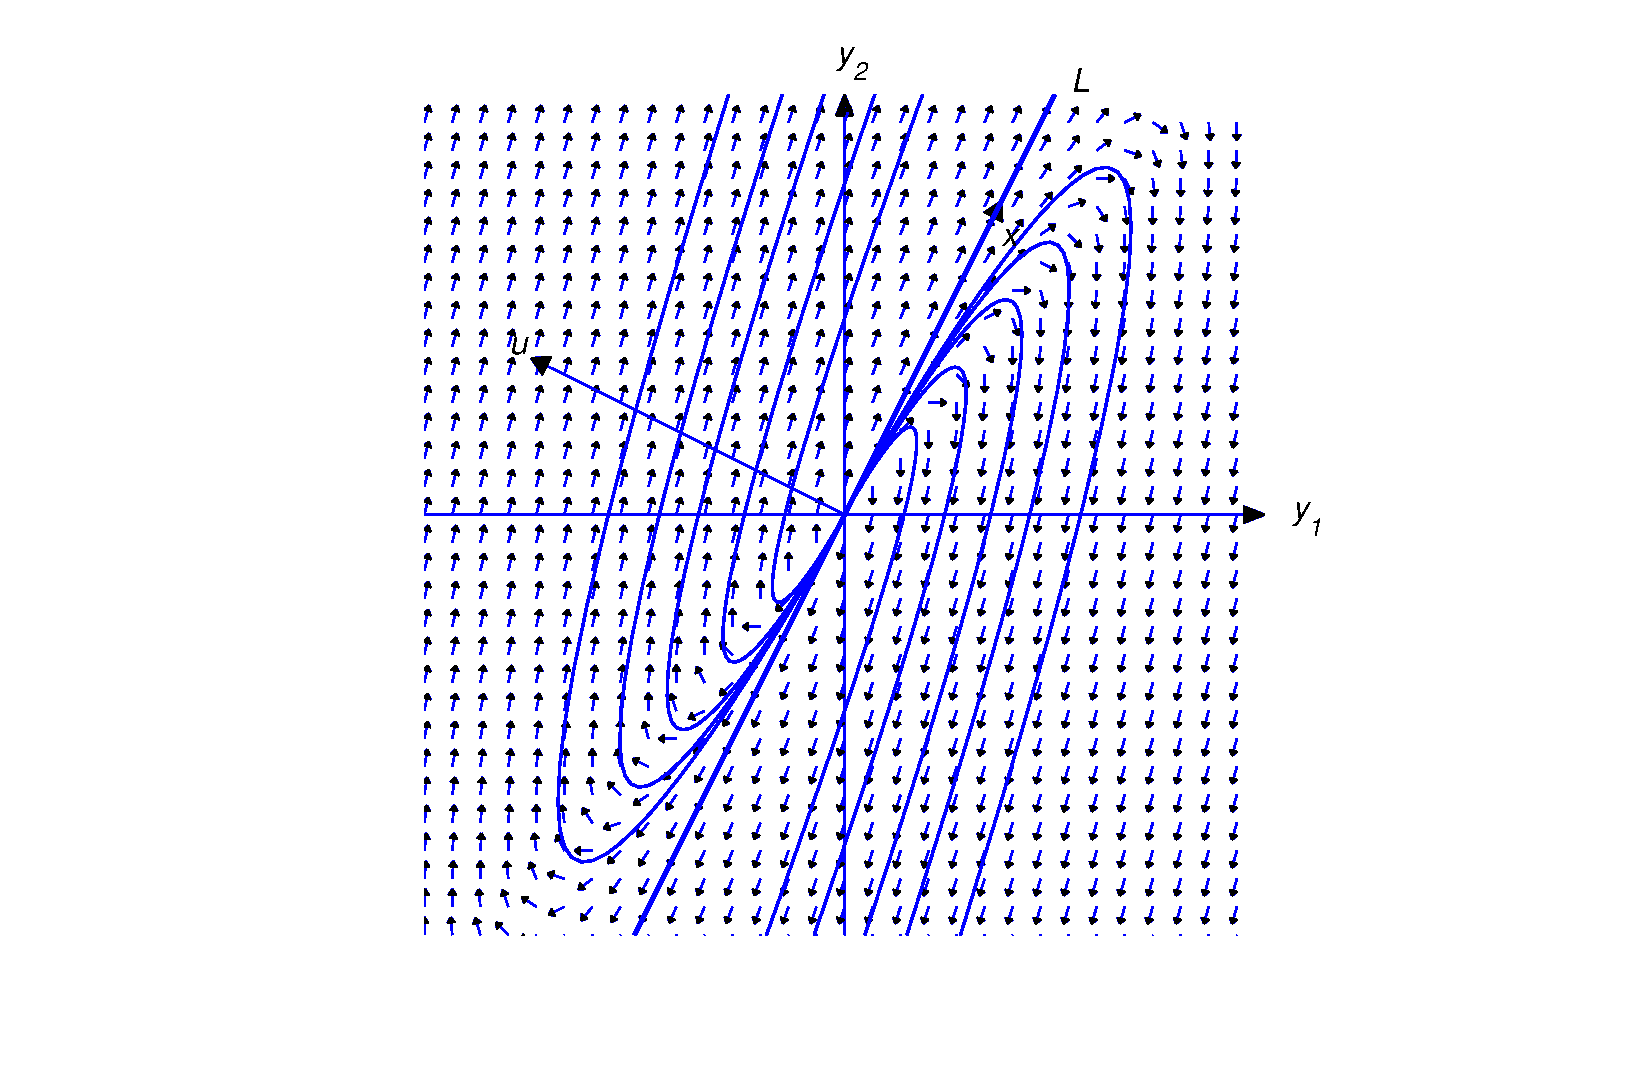
\includegraphics[bb=-78 148 689 643, width=5.67in, height=3.66in, keepaspectratio]{fig100503}}
    \caption{Positive eigenvalue; motion away from the origin}
    \label{figure:10.5.3}
  \end{minipage}
\end{figure}

\begin{figure}[H]
  \color{blue}
  \begin{minipage}[b]{0.5\linewidth}
    \centering
    \scalebox{.65}{
    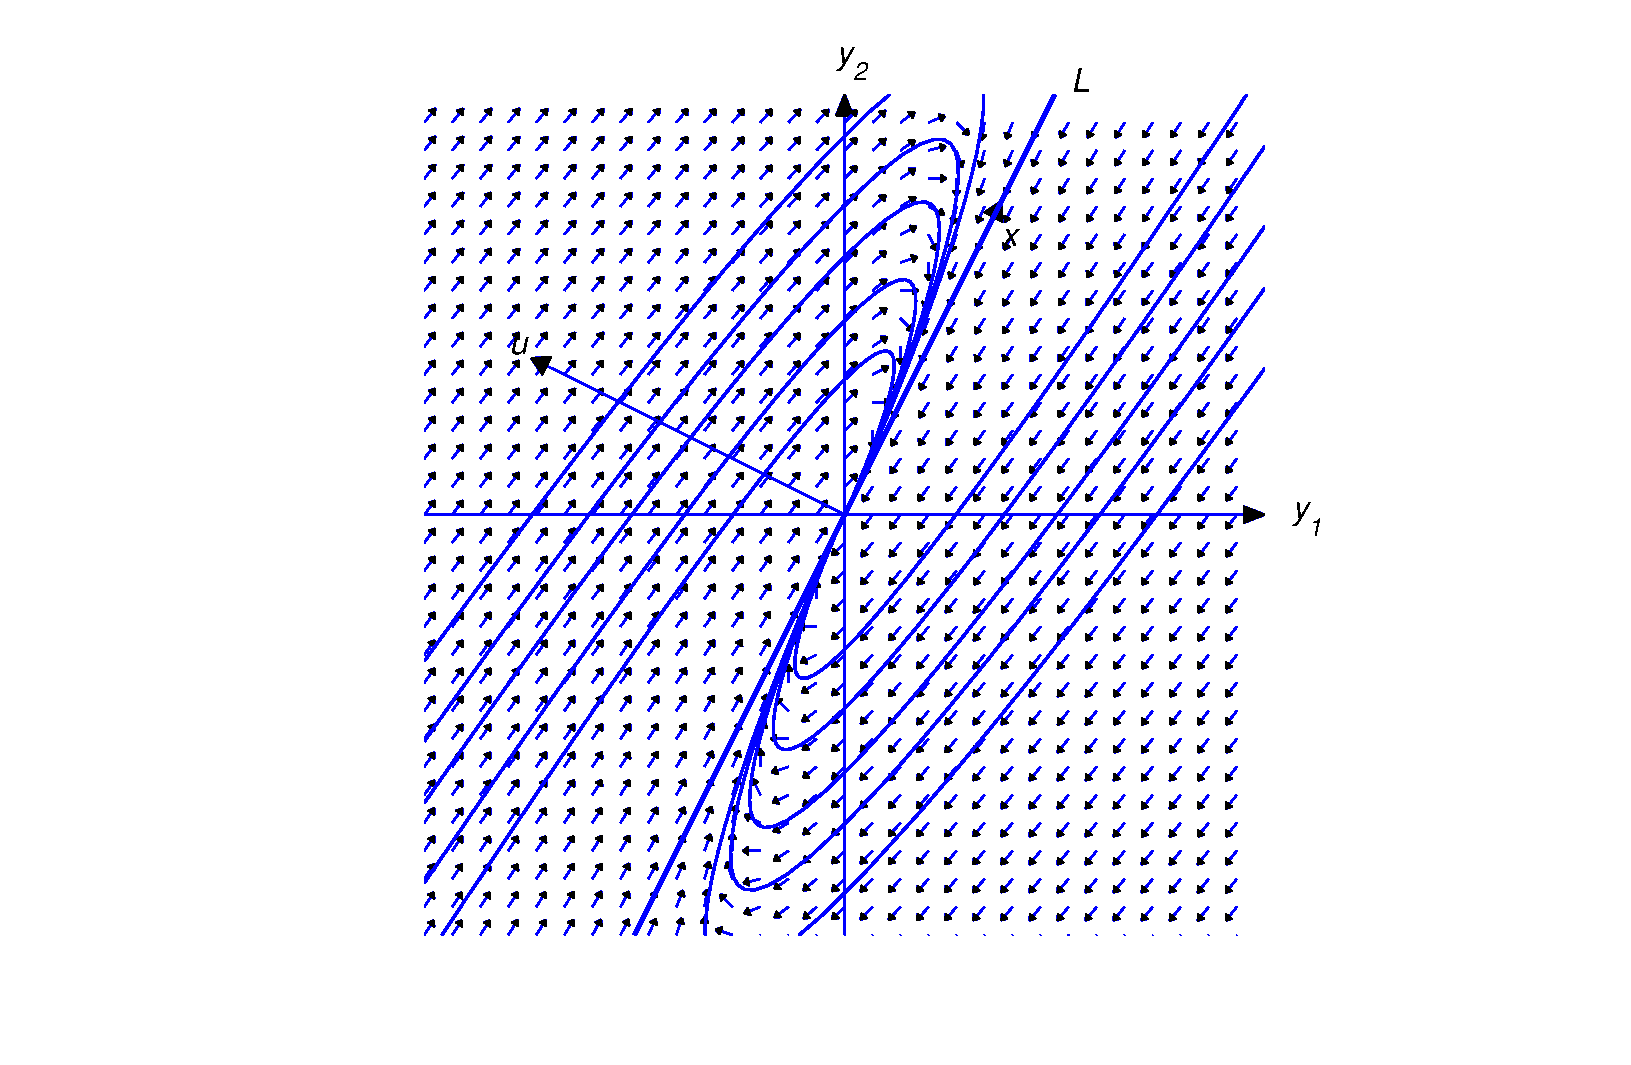
\includegraphics[bb=-78 148 689 643, width=5.67in, height=3.66in, keepaspectratio]{fig100504}
    }
    \caption{Negative eigenvalue; motion toward the origin}
    \label{figure:10.5.4}
  \end{minipage}
  \begin{minipage}[b]{0.5\linewidth}
    \centering
    \scalebox{.65}{
    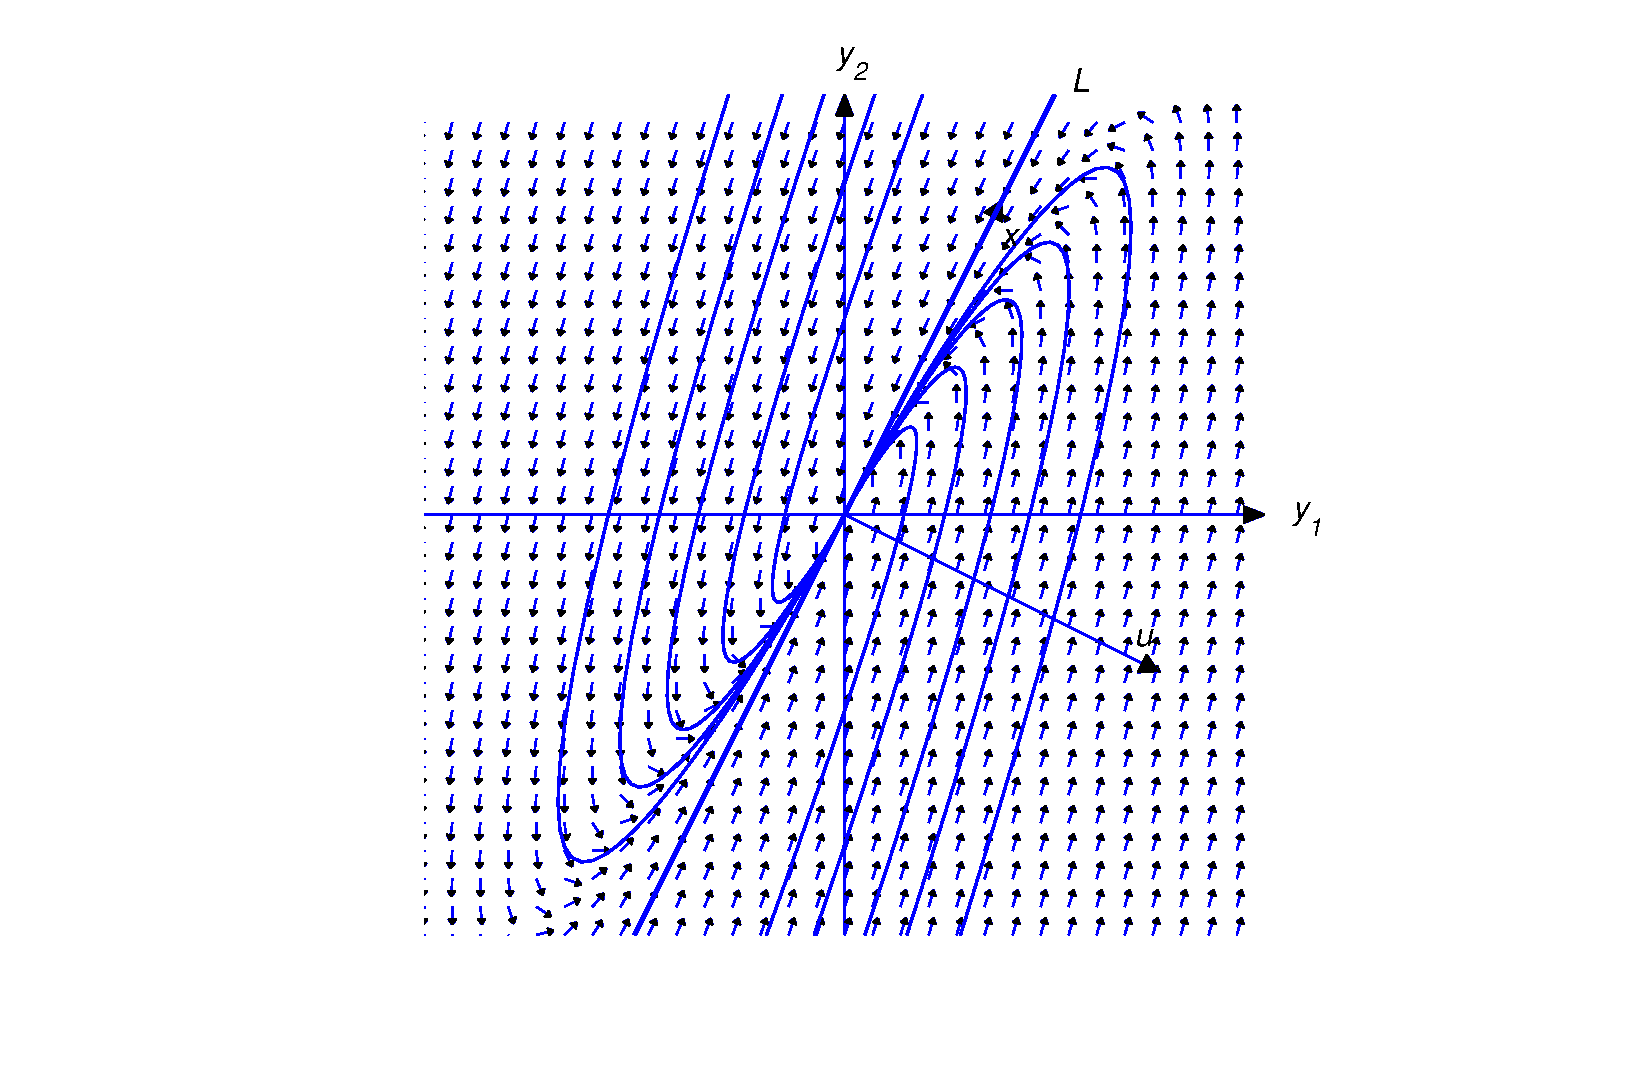
\includegraphics[bb=-78 148 689 643, width=5.67in, height=3.66in, keepaspectratio]{fig100505}
    }
    \caption{Negative eigenvalue; motion toward the origin}
    \label{figure:10.5.5}
  \end{minipage}
\end{figure}

\newpage

\exercises In Exercises~\ref{exer:10.5.1}--\ref{exer:10.5.12} find the general solution.

\begin{exerciselist}
  \begin{tabular}[t]{@{}p{168pt}@{}p{168pt}}
    \item\label{exer:10.5.1} $\dst{{\bf y}'=\twobytwo34{-1}7{\bf y}}$ &
    \item\label{exer:10.5.2} $\dst{{\bf y}'=\twobytwo0{-1}1{-2}{\bf y}}$
  \end{tabular}

  \begin{tabular}[t]{@{}p{168pt}@{}p{168pt}}
    \item\label{exer:10.5.3} $\dst{{\bf y}'=\twobytwo{-7}4{-1}{-11}{\bf y}}$ &
    \item\label{exer:10.5.4} $\dst{{\bf y}'=\twobytwo31{-1}1{\bf y}}$
  \end{tabular}

  \begin{tabular}[t]{@{}p{168pt}@{}p{168pt}}
    \item\label{exer:10.5.5} $\dst{{\bf y}'=\twobytwo4{12}{-3}{-8}{\bf y}}$ &
    \item\label{exer:10.5.6} $\dst{{\bf y'}=\twobytwo{-10}9{-4}2{\bf y}}$
  \end{tabular}

  \begin{tabular}[t]{@{}p{168pt}@{}p{168pt}}
    \item\label{exer:10.5.7} $\dst{{\bf y'}=\twobytwo{-13}{16}{-9}{11}{\bf y}}$ &
    \item\label{exer:10.5.8} $\dst{{\bf y'}=\threebythree021{-4}61042{\bf y}}$
  \end{tabular}

  \begin{tabular}[t]{@{}p{168pt}@{}p{168pt}}
    \item\label{exer:10.5.9} $\dst{{\bf y}'=\frac{1}{3}\threebythree11{-3}{-4}{-4}3{-2}10{\bf y}}$ &
    \item\label{exer:10.5.10} $\dst{{\bf y}' =\threebythree{-1}1{-1}{-2}02{-1}3{-1}{\bf y}}$
  \end{tabular}

  \begin{tabular}[t]{@{}p{168pt}@{}p{168pt}}
    \item\label{exer:10.5.11} $\dst{{\bf y}' =\threebythree4{-2}{-2}{-2}3{-1}2{-1}3{\bf y}}$ &
    \item\label{exer:10.5.12} $\dst{{\bf y}'= \threebythree6{-5}32{-1}3211{\bf y}}$
  \end{tabular}

  \exercisetext{In Exercises~\ref{exer:10.5.13}--\ref{exer:10.5.23} solve the initial value
  problem.}

  \item\label{exer:10.5.13}
        $\dst{{\bf y}'=\twobytwo{-11}8{-2}{-3}{\bf y},\quad{\bf y}(0)=\twocol62}$

  \item\label{exer:10.5.14}
        $\dst{{\bf y}'=\twobytwo{15}{-9}{16}{-9}{\bf y},\quad{\bf y}(0)=\twocol58}$

  \item\label{exer:10.5.15} $\dst{{\bf y}'=\twobytwo{-3}{-4}1{-7}{\bf y},\quad{\bf y}(0)=\twocol23}$

  \item\label{exer:10.5.16}
        $\dst{{\bf y}'=\twobytwo{-7}{24}{-6}{17}{\bf y},\quad{\bf y}(0)=\twocol31}$

  \item\label{exer:10.5.17} $\dst{{\bf y}'=\twobytwo{-7}3{-3}{-1}{\bf y},\quad{\bf y}(0)=\twocol02}$

  \item\label{exer:10.5.18}
        $\dst{{\bf y}' =\threebythree{-1}101{-1}{-2}{-1}{-1}{-1}{\bf y},\quad {\bf y}(0)=\threecol65{-7}}$

  \item\label{exer:10.5.19}
        $\dst{{\bf y}' =\threebythree{-2}21{-2}21{-3}32{\bf y},\quad {\bf y}(0)=\threecol{-6}{-2}0}$

  \item\label{exer:10.5.20}
        $\dst{{\bf y}' =\threebythree{-7}{-4}4{-1}01{-9}{-5}6{\bf y},\quad\bf {\bf y}(0)=\threecol{-6}9{-1}}$

  \item\label{exer:10.5.21}
        $\dst{{\bf y}' =\threebythree{-1}{-4}{-1}361{-3}{-2}3\bf y,\quad\bf y(0)=\threecol{-2}13}$

  \item\label{exer:10.5.22}
        $\dst{{\bf y}' =\threebythree4{-8}{-4}{-3}{-1}{-3}1{-1}9{\bf y},\quad {\bf y}(0)=\threecol{-4}1{-3}}$

  \item\label{exer:10.5.23}
        $\dst{{\bf y}'= \threebythree{-5}{-1}{11}{-7}1{13}{-4}08{\bf y},\quad {\bf y}(0)=\threecol022}$

  \exercisetext{The coefficient matrices in Exercises~\ref{exer:10.5.24}--\ref{exer:10.5.32} have
  eigenvalues of multiplicity $3$. Find the general solution.}

  \begin{tabular}[t]{@{}p{168pt}@{}p{168pt}}
    \item\label{exer:10.5.24} $\dst{{\bf y}' =\threebythree5{-1}1{-1}9{-3}{-2}24{\bf y}}$ &
    \item\label{exer:10.5.25} $\dst{{\bf y}' =\threebythree1{10}{-12}2232{-1}6{\bf y}}$
  \end{tabular}

  \begin{tabular}[t]{@{}p{168pt}@{}p{168pt}}
    \item\label{exer:10.5.26} $\dst{{\bf y}' =\threebythree{-6}{-4}{-4}2{-1}1231{\bf y}}$ &
    \item\label{exer:10.5.27} $\dst{{\bf y}' =\threebythree02{-2}{-1}5{-3}111{\bf y}}$
  \end{tabular}

  \begin{tabular}[t]{@{}p{168pt}@{}p{168pt}}
    \item\label{exer:10.5.28} $\dst{{\bf y}' =\threebythree{-2}{-12}{10}2{-24}{11}2{-24}8{\bf y}}$ &
    \item\label{exer:10.5.29} $\dst{{\bf y}' =\threebythree{-1}{-12}81{-9}41{-6}1{\bf y}}$
  \end{tabular}

  \begin{tabular}[t]{@{}p{168pt}@{}p{168pt}}
    \item\label{exer:10.5.30} $\dst{{\bf y}' =\threebythree{-4}0{-1}{-1}{-3}{-1}10{-2}{\bf y}}$ &
    \item\label{exer:10.5.31} $\dst{{\bf y}' =\threebythree{-3}{-3}445{-8}23{-5}\bf y}$
  \end{tabular}

  \item\label{exer:10.5.32} ${\bf y}'={\threebythree{-3}{-1}01{-1}0{-1}{-1}{-2}}{\bf y}$

  \item\label{exer:10.5.33} Under the assumptions of Theorem~\ref{thmtype:10.5.1}, suppose ${\bf u}$
        and $\hat{\bf u}$ are vectors such that
  \[
    (A-\lambda_{1}I){\bf u}={\bf x}\quad\mbox{and }\quad (A-\lambda_{1}I)\hat{\bf u}={\bf x},
  \]
  and let
  \[
    {\bf y}_{2}={\bf u}e^{\lambda_{1}t}+{\bf x}te^{\lambda_{1}t}\quad\mbox{and }\quad \hat{\bf y}_{2}=\hat{\bf u}e^{\lambda_{1}t}+{\bf x}te^{\lambda_{1}t}.
  \]
  Show that ${\bf y}_{2}-\hat{\bf y}_{2}$ is a scalar multiple of
  ${\bf y}_{1}={\bf x}e^{\lambda_{1}t}$.

  \item\label{exer:10.5.34} Under the assumptions of Theorem~\ref{thmtype:10.5.2}, let
  \begin{eqnarray*}
    {\bf y}_{1} & = & {\bf x}e^{\lambda_{1}t},                                      \\
    {\bf y}_{2} & = & {\bf u}e^{\lambda_{1}t}+{\bf x}te^{\lambda_{1}t},\mbox{ and } \\
    {\bf y}_{3} & = & {\bf v}e^{\lambda_{1}t}+{\bf u}te^{\lambda_{1}t}+{\bf x}{\frac{t^{2}e^{\lambda_{1}t}}{2}}.
  \end{eqnarray*}
  Complete the proof of Theorem~\ref{thmtype:10.5.2} by showing that ${\bf y}_{3}$ is a solution of
  ${\bf y}'=A{\bf y}$ and that $\{{\bf y}_{1},{\bf y}_{2},{\bf y}_{3}\}$ is linearly independent.

  \item\label{exer:10.5.35} Suppose the matrix
  \[
    A=\left[
    \begin{array}{cc}
      a_{11} & a_{12} \\
      a_{21} & a_{22}
    \end{array}\right]
  \]
  has a repeated eigenvalue $\lambda_{1}$ and the associated eigenspace is one-dimensional. Let
  ${\bf x}$ be a $\lambda_{1}$-eigenvector of $A$. Show that if
  $(A-\lambda_{1}I){\bf u}_{1}={\bf x}$ and $(A-\lambda_{1}I){\bf u}_{2}={\bf x}$, then
  ${\bf u}_{2}-{\bf u}_{1}$ is parallel to ${\bf x}$. Conclude from this that all vectors ${\bf u}$
  such that $(A-\lambda_{1}I){\bf u}={\bf x}$ define the same positive and negative half-planes with
  respect to the line $L$ through the origin parallel to ${\bf x}$.

  \exercisetext{In Exercises~\ref{exer:10.5.36}-~\ref{exer:10.5.45} plot trajectories of the given
  system.}
  \begin{tabular}[t]{@{}p{168pt}@{}p{168pt}}
    \item\label{exer:10.5.36} \CGex\, ${\bf y}'=\dst{\twobytwo{-3}{-1}41}{\bf y}$ &
    \item\label{exer:10.5.37} \CGex\, ${\bf y}'=\dst{\twobytwo2{-1}10}{\bf y}$
  \end{tabular}

  \begin{tabular}[t]{@{}p{168pt}@{}p{168pt}}
    \item\label{exer:10.5.38} \CGex\, ${\bf y}'=\dst{\twobytwo{-1}{-3}35}{\bf y}$ &
    \item\label{exer:10.5.39} \CGex\, ${\bf y}'=\dst{\twobytwo{-5}3{-3}1}{\bf y}$
  \end{tabular}

  \begin{tabular}[t]{@{}p{168pt}@{}p{168pt}}
    \item\label{exer:10.5.40} \CGex\, ${\bf y}'=\dst{\twobytwo{-2}{-3}34}{\bf y}$ &
    \item\label{exer:10.5.41} \CGex\, ${\bf y}'=\dst{\twobytwo{-4}{-3}32}{\bf y}$
  \end{tabular}

  \begin{tabular}[t]{@{}p{168pt}@{}p{168pt}}
    \item\label{exer:10.5.42} \CGex\, ${\bf y}'=\dst{\twobytwo0{-1}1{-2}}{\bf y}$ &
    \item\label{exer:10.5.43} \CGex\, ${\bf y}'=\dst{\twobytwo01{-1}2}{\bf y}$
  \end{tabular}

  \begin{tabular}[t]{@{}p{168pt}@{}p{168pt}}
    \item\label{exer:10.5.44} \CGex\, ${\bf y}'=\dst{\twobytwo{-2}1{-1}0}{\bf y}$ &
    \item\label{exer:10.5.45} \CGex\, ${\bf y}'=\dst{\twobytwo0{-4}1{-4}}{\bf y}$
  \end{tabular}
\end{exerciselist}


\section{Constant Coefficient Homogeneous Systems III}

\noindent
We now consider the system ${\bf y}'=A{\bf y}$, where $A$ has a complex
eigenvalue $\lambda=\alpha+i\beta$ with $\beta\ne0$. We continue to
assume that $A$ has real entries, so the characteristic polynomial of
$A$ has real coefficients. This implies that
$\overline\lambda=\alpha-i\beta$ is also an eigenvalue of $A$.

An eigenvector ${\bf x}$ of $A$ associated with
$\lambda=\alpha+i\beta$ will have complex entries, so we'll write
$$
{\bf x}={\bf u}+i{\bf v}
$$
where ${\bf u}$ and ${\bf v}$ have real entries; that is, ${\bf u}$
and ${\bf v}$ are the real and imaginary parts of ${\bf x}$. Since
$A{\bf x}=\lambda {\bf x}$,
\begin{equation} \label{eq:10.6.1}
A({\bf u}+i{\bf v})=(\alpha+i\beta)({\bf u}+i{\bf v}).
\end{equation}
Taking complex conjugates here and recalling that $A$ has real entries
yields
$$
A({\bf u}-i{\bf v})=(\alpha-i\beta)({\bf u}-i{\bf v}),
$$
which shows that ${\bf x}={\bf u}-i{\bf v}$ is an eigenvector
associated with $\overline\lambda=\alpha-i\beta$. The complex
conjugate eigenvalues $\lambda$ and $\overline\lambda$ can be
separately associated with linearly independent solutions ${\bf
y}'=A{\bf y}$;     however, we won't pursue this approach, since solutions
obtained in this way turn out to be complex--valued. Instead, we'll
obtain solutions of ${\bf y}'=A{\bf y}$ in the form
\begin{equation} \label{eq:10.6.2}
{\bf y}=f_1{\bf u}+f_2{\bf v}
\end{equation}
where $f_1$ and $f_2$ are real--valued scalar functions.
The next theorem shows how to do this.

\begin{theorem}\color{blue} \label{thmtype:10.6.1}
Let $A$ be an $n\times n$ matrix with real entries$.$ Let
$\lambda=\alpha+i\beta$ {\rm(}$\beta\ne0${\rm}) be a complex
eigenvalue of $A$ and let ${\bf x}={\bf u}+i{\bf v}$ be an associated
eigenvector$,$ where ${\bf u}$ and ${\bf v}$ have real components$.$ Then
${\bf u}$ and ${\bf v}$ are both nonzero and
$$
{\bf y}_1=e^{\alpha t}({\bf u}\cos\beta t-{\bf v}\sin\beta t)
\mbox{\quad and\quad}
{\bf y}_2=e^{\alpha t}({\bf u}\sin\beta t+{\bf v}\cos\beta t),
$$
which are the real and imaginary parts of
\begin{equation} \label{eq:10.6.3}
e^{\alpha t}(\cos\beta t+i\sin\beta t)({\bf u}+i{\bf v}),
\end{equation}
are linearly independent solutions of  ${\bf y}'=A{\bf y}$.
\end{theorem}

\proof
A function of the form \eqref{eq:10.6.2} is a solution of ${\bf y}'=A{\bf
y}$ if and only if
\begin{equation} \label{eq:10.6.4}
f_1'{\bf u}+f_2'{\bf
v}=f_1A{\bf u}+f_2A{\bf v}.
\end{equation}
Carrying out the multiplication indicated on the  right side
of \eqref{eq:10.6.1} and collecting the  real and imaginary parts of the
result yields
$$
A({\bf u}+i{\bf v})=(\alpha{\bf u}-\beta{\bf v})+i(\alpha{\bf v}+\beta{\bf
u}).
$$
Equating real and imaginary parts on the two sides of this equation yields
$$
\begin{array}{rcl}
A{\bf u}&=&\alpha{\bf u}-\beta{\bf v}\\
A{\bf v}&=&\alpha{\bf v}+\beta{\bf u}.
\end{array}
$$
We leave it to you (Exercise~\ref{exer:10.6.25}) to show from this that
${\bf u}$ and
${\bf v}$ are both nonzero.
Substituting from these equations into \eqref{eq:10.6.4} yields
\begin{eqnarray*}
f_1'{\bf u}+f_2'{\bf v}
&=&f_1(\alpha{\bf u}-\beta{\bf v})+f_2(\alpha{\bf v}+\beta{\bf u})\\
&=&(\alpha f_1+\beta f_2){\bf u}+(-\beta f_1+\alpha f_2){\bf v}.
\end{eqnarray*}
This is true if
$$
\begin{array}{rcr}
f_1'&=&\alpha f_1+\beta f_2\phantom{,}\\
f_2'&=&-\beta f_1+\alpha f_2,
\end{array}
\mbox{\quad or, equivalently,\quad}
\begin{array}{rcr}
f_1'-\alpha f_1&=&\phantom{-}\beta f_2\phantom{.}\\
f_2'-\alpha f_2&=&-\beta f_1.
\end{array}
$$
If we let $f_1=g_1e^{\alpha t}$ and $f_2=g_2e^{\alpha t}$, where
$g_1$ and $g_2$ are to be determined, then the last two equations
become
$$
\begin{array}{rcr}
g_1'&=&\beta g_2\phantom{.}\\
g_2'&=&-\beta g_1,
\end{array}
$$
which implies that
$$
g_1''=\beta g_2'=-\beta^2 g_1,
$$
so
$$
g_1''+\beta^2 g_1=0.
$$
The general solution of this equation is
$$
g_1=c_1\cos\beta t+c_2\sin\beta t.
$$
Moreover, since $g_2=g_1'/\beta$,
$$
g_2=-c_1\sin\beta t+c_2\cos\beta t.
$$
Multiplying  $g_1$  and $g_2$  by $e^{\alpha t}$ shows that
\begin{eqnarray*}
f_1&=&e^{\alpha t}(\phantom{-}c_1\cos\beta t+c_2\sin\beta t ),\\
f_2&=&e^{\alpha t}(-c_1\sin\beta t+c_2\cos\beta t).
\end{eqnarray*}
Substituting these into \eqref{eq:10.6.2} shows that
\begin{equation} \label{eq:10.6.5}
\begin{array}{rcl}
{\bf y}&=&e^{\alpha t}\left[(c_1\cos\beta t+c_2\sin\beta t){\bf u}
+(-c_1\sin\beta t+c_2\cos\beta t){\bf v}\right]\\
&=&c_1e^{\alpha t}({\bf u}\cos\beta t-{\bf v}\sin\beta t)
+c_2e^{\alpha t}({\bf u}\sin\beta t+{\bf v}\cos\beta t)
\end{array}
\end{equation}
is a solution of ${\bf y}'=A{\bf y}$ for any choice of the constants
$c_1$ and $c_2$. In particular, by first taking $c_1=1$ and $c_2=0$
and then taking $c_1=0$ and $c_2=1$, we see that ${\bf y}_1$ and ${\bf
y}_2$ are solutions of $ {\bf y}'=A{\bf y}$. We leave it to you to
verify that they are, respectively, the real and imaginary parts of
\eqref{eq:10.6.3} (Exercise~\ref{exer:10.6.26}), and that they are linearly
independent (Exercise~\ref{exer:10.6.27}).

\begin{example}\label{example:10.6.1} \rm
 Find the general solution of
\begin{equation} \label{eq:10.6.6}
{\bf y}'=\twobytwo4{-5}5{-2}{\bf y}.
\end{equation}
\end{example}

\solution The characteristic polynomial of the coefficient matrix $A$
in \eqref{eq:10.6.6} is
$$
\left|\begin{array}{cc} 4-\lambda&-5\\ 5&-2-\lambda
\end{array}\right|=(\lambda-1)^2+16.
$$
Hence, $\lambda=1+4i$ is an eigenvalue of $A$. The associated
eigenvectors satisfy $\left(A-\left(1+4i\right)I\right){\bf x}={\bf
0}$. The augmented matrix of this system is
$$
\left[\begin{array}{cccr} 3-4i&-5&\vdots&0\\
5&-3-4i&\vdots&0  \end{array}\right],
 $$
which is row equivalent to
$$
\left[\begin{array}{cccr} 1&-{3+4i\over5}&\vdots&0\\ 0&0&\vdots&0
\end{array}\right].
$$
Therefore $x_1=(3+4i)x_2/5$. Taking $x_2=5$ yields $x_1=3+4i$, so
$$
{\bf x}=\left[\begin{array}{c}3+4i\\5\end{array}\right]
$$
is an eigenvector.  The real and imaginary parts of
$$
e^t(\cos4t+i\sin4t)\left[\begin{array}{c}3+4i\\5\end{array}\right]
$$
 are
$$
{\bf y}_1=e^t\left[\begin{array}{c}3\cos4t-4\sin
4t\\5\cos4t\end{array}\right]\quad\mbox{ and }\quad
{\bf y}_2=e^t\left[\begin{array}{c}3\sin4t+4\cos4t\\5\sin
4t\end{array}\right],
$$
which are linearly independent solutions of  \eqref{eq:10.6.6}.
The general solution of \eqref{eq:10.6.6} is
$$
{\bf y}=
c_1e^t\left[\begin{array}{c}3\cos4t-4\sin
4t\\5\cos4t\end{array}\right]+
c_2e^t\left[\begin{array}{c}3\sin4t+4\cos4t\\5\sin
4t\end{array}\right].
$$

\begin{example}\label{example:10.6.2} \rm
 Find  the general solution of
\begin{equation} \label{eq:10.6.7}
{\bf y}'=\twobytwo{-14}{39}{-6}{16}{\bf y}.
\end{equation}
\end{example}

\solution The characteristic polynomial of the coefficient matrix $A$
in \eqref{eq:10.6.7} is
$$
\left|\begin{array}{cc}-14-\lambda&39\\-6&16-\lambda
\end{array}\right|=(\lambda-1)^2+9.
$$
Hence, $\lambda=1+3i$ is an eigenvalue of $A$. The associated
eigenvectors satisfy $\left(A-(1+3i)I\right){\bf x}={\bf 0}$. The
augmented matrix of this system is
$$
\left[\begin{array}{cccr}-15-3i&39&\vdots&0\\
-6&15-3i&\vdots&0  \end{array}\right],
 $$
which is row equivalent to
$$
\left[\begin{array}{cccr} 1&{-5+i\over2}&\vdots&0\\ 0&0&\vdots&0
\end{array}\right].
$$
Therefore $x_1=(5-i)/2$. Taking $x_2=2$ yields $x_1=5-i$, so
$$
{\bf x}=\left[\begin{array}{c}5-i\\2\end{array}\right]
$$
is an eigenvector. The real and imaginary parts of
$$
e^t(\cos3t+i\sin3t)\left[\begin{array}{c}5-i\\2\end{array}\right]
$$
 are
$$
{\bf y}_1=e^t\left[\begin{array}{c}\sin3t+5\cos3t\\2\cos
3t\end{array}\right]\quad\mbox{ and }\quad
{\bf y}_2=e^t\left[\begin{array}{c}-\cos3t+5\sin3t\\2\sin
3t\end{array}\right],
 $$
which are  linearly independent solutions of  \eqref{eq:10.6.7}.
The general solution of \eqref{eq:10.6.7} is
$$
{\bf y}=c_1e^t\left[\begin{array}{c}\sin3t+5\cos3t\\2\cos
3t\end{array}\right]+
c_2e^t\left[\begin{array}{c}-\cos3t+5\sin3t\\2\sin
3t\end{array}\right].
$$

\begin{example}\label{example:10.6.3}  \rm
 Find the general solution of
\begin{equation} \label{eq:10.6.8}
{\bf y}'=\threebythree{-5}54{-8}76100{\bf y}.
\end{equation}
\end{example}

\solution  The characteristic
polynomial of the  coefficient matrix $A$ in  \eqref{eq:10.6.8} is
$$
\left|\begin{array}{ccc}-5-\lambda&5&4\\-8&7-\lambda&
6\\ \phantom{-}1
&0&-\lambda\end{array}\right|=-(\lambda-2)(\lambda^2+1).
$$
Hence, the eigenvalues of $A$ are $\lambda_1=2$, $\lambda_2=i$, and
$\lambda_3=-i$.
The augmented matrix of $(A-2I){\bf x=0}$ is
$$
\left[\begin{array}{rrrcr}-7&5&4&\vdots&0\\-8&
5&6&\vdots&0\\ 1&0&-2&\vdots&0
\end{array}\right],
$$
which is row equivalent to
$$
\left[\begin{array}{rrrcr} 1&0&-2&\vdots&0\\ 0&1&-2&
\vdots&0\\ 0&0&0&\vdots&0\end{array}\right].
$$
Therefore $x_1=x_2=2x_3$.  Taking $x_3=1$ yields
$$
{\bf x}_1=\threecol221,
$$
so
$$
{\bf y}_1=\threecol221e^{2t}
$$
is a solution of  \eqref{eq:10.6.8}.

The augmented  matrix of $(A-iI){\bf x=0}$ is
$$
\left[\begin{array}{ccrccc}-5-i&5&4&\vdots&0\\-8&
7-i&6&\vdots&0\\ \phantom{-}1&0&-i&\vdots&0
\end{array}\right],
$$
which is row equivalent to
$$
\left[\begin{array}{ccccc} 1&0&-i&\vdots&0\\ 0&1&1-i&
\vdots&0\\ 0&0&0&\vdots&0\end{array}\right].
$$
Therefore $x_1=ix_3$ and $x_2=-(1-i)x_3$. Taking $x_3=1$ yields
the eigenvector
$$
{\bf x}_2=\left[\begin{array}{c} i\\-1+i\\ 1\end{array}
\right].
$$
The real and imaginary parts of
$$
(\cos t+i\sin t)\left[\begin{array}{c}i\\-1+i\\1\end{array}\right]
$$
 are
$$
{\bf y}_2=
\left[\begin{array}{c}-\sin t\\-\cos t-\sin t\\\cos t\end{array}\right]
\quad\mbox{ and }\quad
{\bf y}_3=\left[\begin{array}{c}\cos t\\\cos t-\sin t\\\sin
t\end{array}\right],
 $$
which are solutions of  \eqref{eq:10.6.8}.
Since the  Wronskian of $\{{\bf y}_1,{\bf y}_2,{\bf y}_3\}$
at $t=0$  is
$$
\left|\begin{array}{rrr}
2&0&1\\2&-1&1\\1&1&0\end{array}\right|=1,
$$
 $\{{\bf y}_1,{\bf y}_2,{\bf y}_3\}$ is a
fundamental set of solutions of \eqref{eq:10.6.8}. The general solution of
\eqref{eq:10.6.8} is
$$
{\bf y}=c_1 \threecol221e^{2t}
+c_2\left[\begin{array}{c}-\sin t\\-\cos t-\sin t\\\cos t\end{array}\right]
+c_3\left[\begin{array}{c}\cos t\\\cos t-\sin t\\\sin
t\end{array}\right].
$$

\begin{example}\label{example:10.6.4}  \rm
 Find the general solution of
\begin{equation} \label{eq:10.6.9}
{\bf y}'=\threebythree1{-1}{-2}1321{-1}2{\bf y}.
\end{equation}
\end{example}

\solution The characteristic
polynomial of the  coefficient matrix $A$ in  \eqref{eq:10.6.9} is
$$
\left|\begin{array}{ccc} 1-\lambda&-1&-2\\ 1&3-\lambda&
\phantom{-}2\\ 1
&-1&2-\lambda\end{array}\right|=
-(\lambda-2)\left((\lambda-2)^2+4\right).
 $$
Hence, the eigenvalues of $A$ are $\lambda_1=2$, $\lambda_2=2+2i$,
and $\lambda_3=2-2i$.
The augmented matrix of $(A-2I){\bf x=0}$ is
$$
\left[\begin{array}{rrrcr}-1&-1&-2&\vdots&0\\1&
1&2&\vdots&0\\ 1&-1&0&\vdots&0
\end{array}\right],
$$
which is row equivalent to
$$
\left[\begin{array}{rrrcr} 1&0&1&\vdots&0\\ 0&1&1&
\vdots&0\\ 0&0&0&\vdots&0\end{array}\right].
$$
Therefore $x_1=x_2=-x_3$.  Taking $x_3=1$ yields
$$
{\bf x}_1=\threecol{-1}{-1}1,
$$
so
$$
{\bf y}_1=\threecol{-1}{-1}1e^{2t}
$$
is a solution of  \eqref{eq:10.6.9}.

The augmented  matrix of $\left(A-(2+2i)I\right){\bf x=0}$ is
$$
\left[\begin{array}{ccrcc}-1-2i&-1&-2&\vdots&0\\ 1&
1-2i&\phantom{-}2&\vdots&0\\ 1&-1&-2i&\vdots&0
\end{array}\right],
$$
which is row equivalent to
$$
\left[\begin{array}{rrrcr} 1&0&-i&\vdots&0\\ 0&1&i&
\vdots&0\\ 0&0&0&\vdots&0\end{array}\right].
$$
Therefore $x_1=ix_3$ and $x_2=-ix_3$. Taking $x_3=1$ yields
the eigenvector
$$
{\bf x}_2=\threecol i{-i}1
$$
The real and imaginary parts of
$$
e^{2t}(\cos2t+i\sin2t)\threecol i{-i}1
$$
are
$$
{\bf y}_2=e^{2t}\left[\begin{array}{r}-\sin2t\\\sin2t\\\cos
2t\end{array}\right]\quad\mbox{ and }\quad
{\bf y}_2=e^{2t}\left[\begin{array}{r}\cos2t\\-\cos2t\\\sin
2t\end{array}\right],
$$
which are solutions of  \eqref{eq:10.6.9}.
Since  the Wronskian of $\{{\bf y}_1,{\bf y}_2,{\bf y}_3\}$
at $t=0$ is
$$
\left|\begin{array}{rrr}
-1&0&1\\-1&0&-1\\1&1&0\end{array}\right|=-2,
$$
$\{{\bf y}_1,{\bf y}_2,{\bf y}_3\}$ is a fundamental set of solutions
of \eqref{eq:10.6.9}.  The general solution of \eqref{eq:10.6.9} is
$$
{\bf y}=c_1\threecol{-1}{-1}1e^{2t}+
c_2e^{2t}\left[\begin{array}{r}-\sin2t\\\sin2t\\\cos
2t\end{array}\right]+
c_3e^{2t}\left[\begin{array}{r}\cos2t\\-\cos2t\\\sin
2t\end{array}\right].
$$

\boxit{Geometric Properties of Solutions when  $n=2$}

\noindent
We'll now  consider the geometric properties of solutions of a
$2\times2$ constant coefficient system
\begin{equation} \label{eq:10.6.10}
\twocol{y_1'}{y_2'}=\left[\begin{array}{cc}a_{11}&a_{12}\\a_{21}&a_{22}
\end{array}\right]\twocol{y_1}{y_2}
\end{equation}
under the assumptions of this section; that is, when the matrix
$$
A=\left[\begin{array}{cc}a_{11}&a_{12}\\a_{21}&a_{22}
\end{array}\right]
$$
has a complex eigenvalue $\lambda=\alpha+i\beta$
{\rm(}$\beta\ne0${\rm}) and ${\bf x}={\bf u}+i{\bf v}$ is an
associated eigenvector, where ${\bf u}$ and ${\bf v}$ have real
components. To describe the trajectories accurately it's necessary to
introduce a new rectangular coordinate system in the $y_1$-$y_2$
plane. This raises a point that hasn't come up before: It is always
possible to choose ${\bf x}$ so that $({\bf u},{\bf v})=0$. A special
effort is required to do this, since not every eigenvector has this
property. However, if we know an eigenvector that doesn't, we can
multiply it by a suitable complex constant to obtain one that does. To
see this, note that if ${\bf x}$ is a $\lambda$-eigenvector of $A$ and
$k$ is an arbitrary real number, then
$$
{\bf x}_1=(1+ik){\bf x}=(1+ik)({\bf u}+i{\bf v})
=({\bf u}-k{\bf v})+i({\bf v}+k{\bf u})
$$
is also a $\lambda$-eigenvector of $A$, since
$$
A{\bf x}_1= A((1+ik){\bf x})=(1+ik)A{\bf x}=(1+ik)\lambda{\bf x}=
\lambda((1+ik){\bf x})=\lambda{\bf x}_1.
$$
The real and imaginary parts of ${\bf x}_1$ are
\begin{equation} \label{eq:10.6.11}
{\bf u}_1={\bf u}-k{\bf v} \mbox{\quad and \quad}
{\bf v}_1={\bf v}+k{\bf u},
\end{equation}
so
$$
({\bf u}_1,{\bf v}_1)=({\bf u}-k{\bf v},{\bf v}+k{\bf u})
=-\left[({\bf u},{\bf v})k^2+(\|{\bf v}\|^2-\|{\bf u}\|^2)k
-({\bf u},{\bf v})\right].
$$
Therefore $({\bf u}_1,{\bf v}_1)=0$ if
\begin{equation} \label{eq:10.6.12}
({\bf u},{\bf v})k^2+(\|{\bf v}\|^2-\|{\bf u}\|^2)k-({\bf u},{\bf
v})=0.
\end{equation}
If $({\bf u},{\bf v})\ne0$ we can use the quadratic formula to find
two real values of $k$ such that $({\bf u}_1,{\bf v}_1)=0$
(Exercise~\ref{exer:10.6.28}).

\begin{example}\label{example:10.6.5} \rm  In Example~\ref{example:10.6.1}
we found the eigenvector
$$
{\bf x}=\ctwocol{3+4i}5=\twocol35+i\twocol40
$$
for the matrix of the system \eqref{eq:10.6.6}. Here ${\bf u}=\dst{\twocol35}$
and ${\bf v}=\twocol40$ are not orthogonal, since $({\bf u},{\bf
v})=12$. Since $\|{\bf v}\|^2-\|{\bf u}\|^2=-18$, \eqref{eq:10.6.12} is
equivalent to
$$
2k^2-3k-2=0.
$$
The zeros of this equation are $k_1=2$ and $k_2=-1/2$. Letting $k=2$
in \eqref{eq:10.6.11} yields
$$
{\bf u}_1={\bf u}-2{\bf v}=\twocol{-5}{\phantom{-}5}\mbox{\quad and \quad}
{\bf v}_1={\bf v}+2{\bf u}=\twocol{10}{10},
$$
and $({\bf u}_1,{\bf v}_1)=0$.
 Letting $k=-1/2$
in \eqref{eq:10.6.11} yields
$$
{\bf u}_1={\bf u}+{{\bf v}\over2}=\twocol{5}5\mbox{\quad and \quad}
{\bf v}_1={\bf v}-{{\bf u}\over2}={1\over2}\twocol{-5}{\phantom{-}5},
$$
and again $({\bf u}_1,{\bf v}_1)=0$. \bbox
\end{example}

(The numbers don't always work out as nicely as in this example.
You'll need a calculator or computer to do
Exercises~\ref{exer:10.6.29}-\ref{exer:10.6.40}.)

Henceforth, we'll assume that $({\bf u},{\bf v})=0$. Let ${\bf U}$ and
${\bf V}$ be unit vectors in the directions of ${\bf u}$ and ${\bf
v}$, respectively; that is, ${\bf U}={\bf u}/\|{\bf u}\|$ and ${\bf
V}={\bf v}/\|{\bf v}\|$. The new rectangular coordinate system will
have the same origin as the $y_1$-$y_2$ system. The coordinates of a
point in this system will be denoted by $(z_1,z_2)$, where $z_1$ and
$z_2$ are the displacements in the directions of ${\bf U}$ and ${\bf
V}$, respectively.

From \eqref{eq:10.6.5}, the solutions of \eqref{eq:10.6.10} are given by
\begin{equation} \label{eq:10.6.13} {\bf y}=e^{\alpha t}\left[(c_1\cos\beta
t+c_2\sin\beta t){\bf u} +(-c_1\sin\beta t+c_2\cos\beta t){\bf
v}\right]. \end{equation} For convenience, let's call the curve
traversed by $e^{-\alpha t}{\bf y}(t)$ a {\color{blue}\it shadow trajectory\/} of
\eqref{eq:10.6.10}. Multiplying \eqref{eq:10.6.13} by $e^{-\alpha t}$ yields
$$
e^{-\alpha t}{\bf y}(t)=z_1(t){\bf U}+z_2(t){\bf V},
$$
where
\begin{eqnarray*}
z_1(t)&=&\|{\bf u}\|(c_1\cos\beta t+c_2\sin\beta
t)\\ z_2(t)&=&\|{\bf v}\|(-c_1\sin\beta t+c_2\cos\beta t).
\end{eqnarray*}
Therefore
$$ {(z_1(t))^2\over\|{\bf
u}\|^2}+{(z_2(t))^2\over\|{\bf v}\|^2} =c_1^2+c_2^2
$$
(verify!), which means that the shadow trajectories of \eqref{eq:10.6.10}
are ellipses centered at the origin, with axes of symmetry parallel to
${\bf U}$ and ${\bf V}$. Since
$$
z_1'={\beta\|{\bf u}\|\over\|{\bf v}\|} z_2\mbox{\quad and \quad}
z_2'=-{\beta\|{\bf v}\|\over\|{\bf u}\|} z_1,
$$
 the vector from the
origin to a point on the shadow ellipse rotates in the same direction
that ${\bf V}$ would have to be rotated by $\pi/2$ radians to bring it
into coincidence with ${\bf U}$ (Figures~\ref{figure:10.6.1} and
\ref{figure:10.6.2}).

\enlargethispage{3in}
\begin{figure}[H]
\color{blue}
  \begin{minipage}[b]{0.5\linewidth}
    \centering
   \scalebox{.65}{
  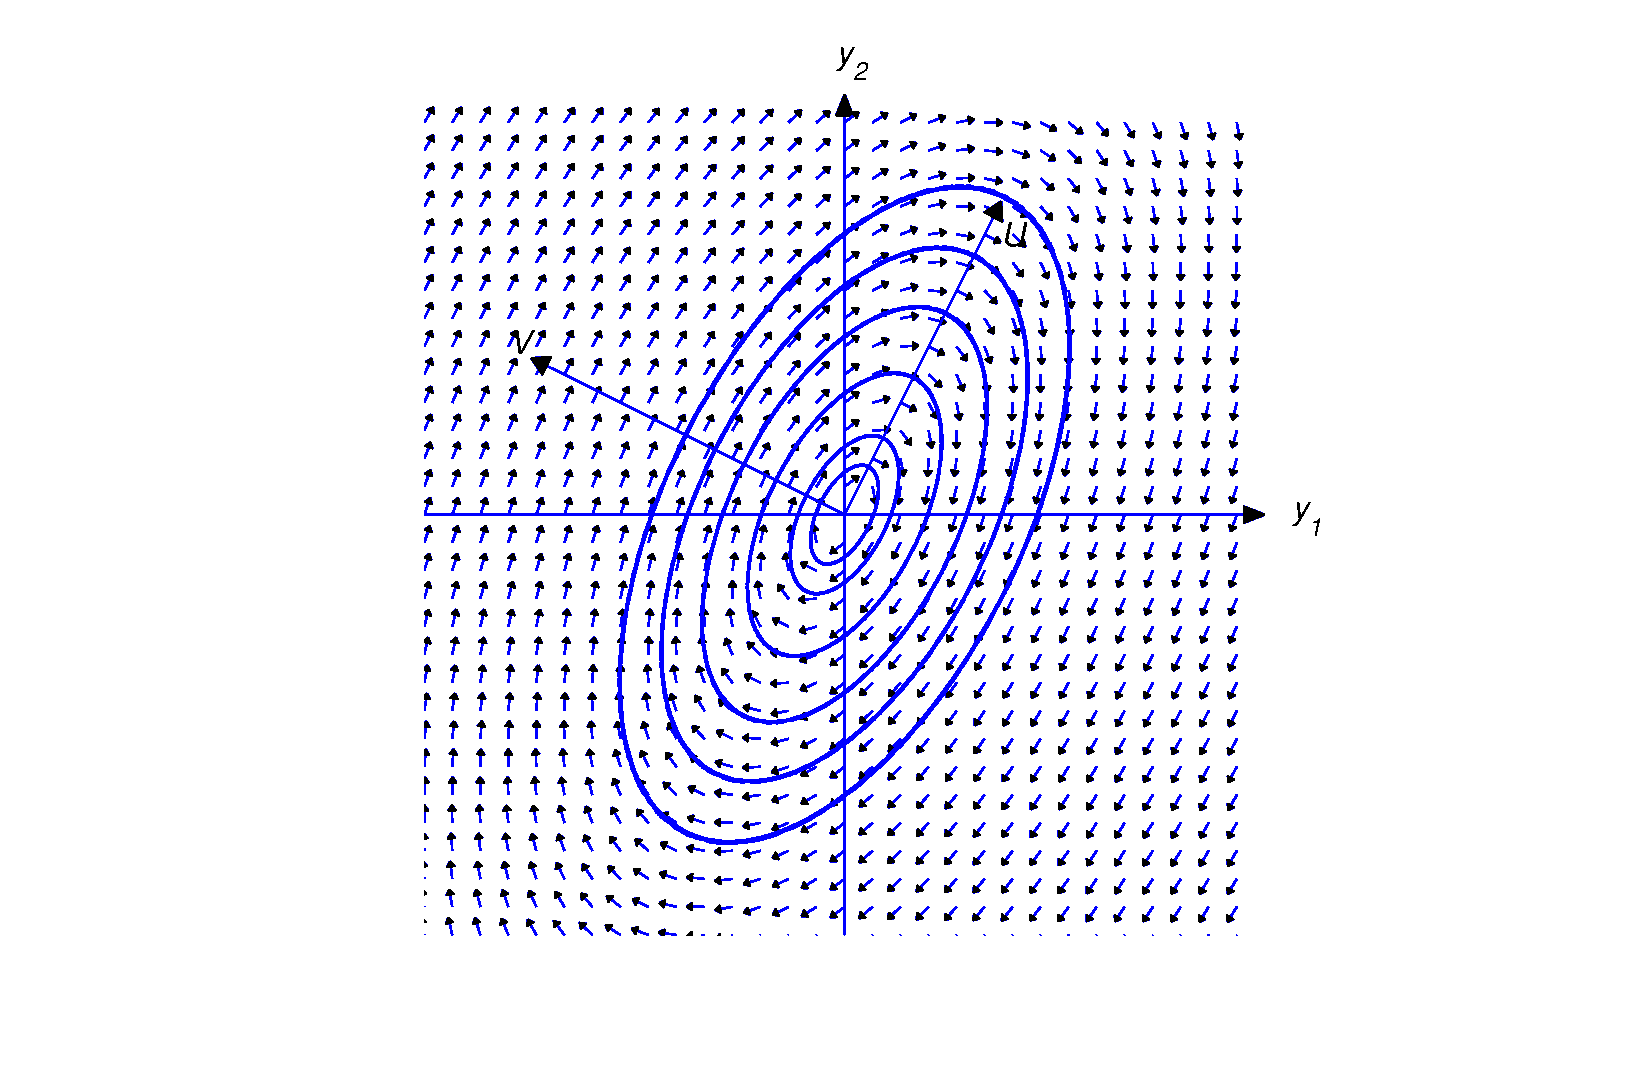
\includegraphics[bb=-78 148 689 643,width=5.67in,height=3.66in,keepaspectratio]{fig100601}}
\caption{ Shadow trajectories traversed clockwise}
  \label{figure:10.6.1}
\end{minipage}
  \begin{minipage}[b]{0.5\linewidth}
    \centering
   \scalebox{.65}{
  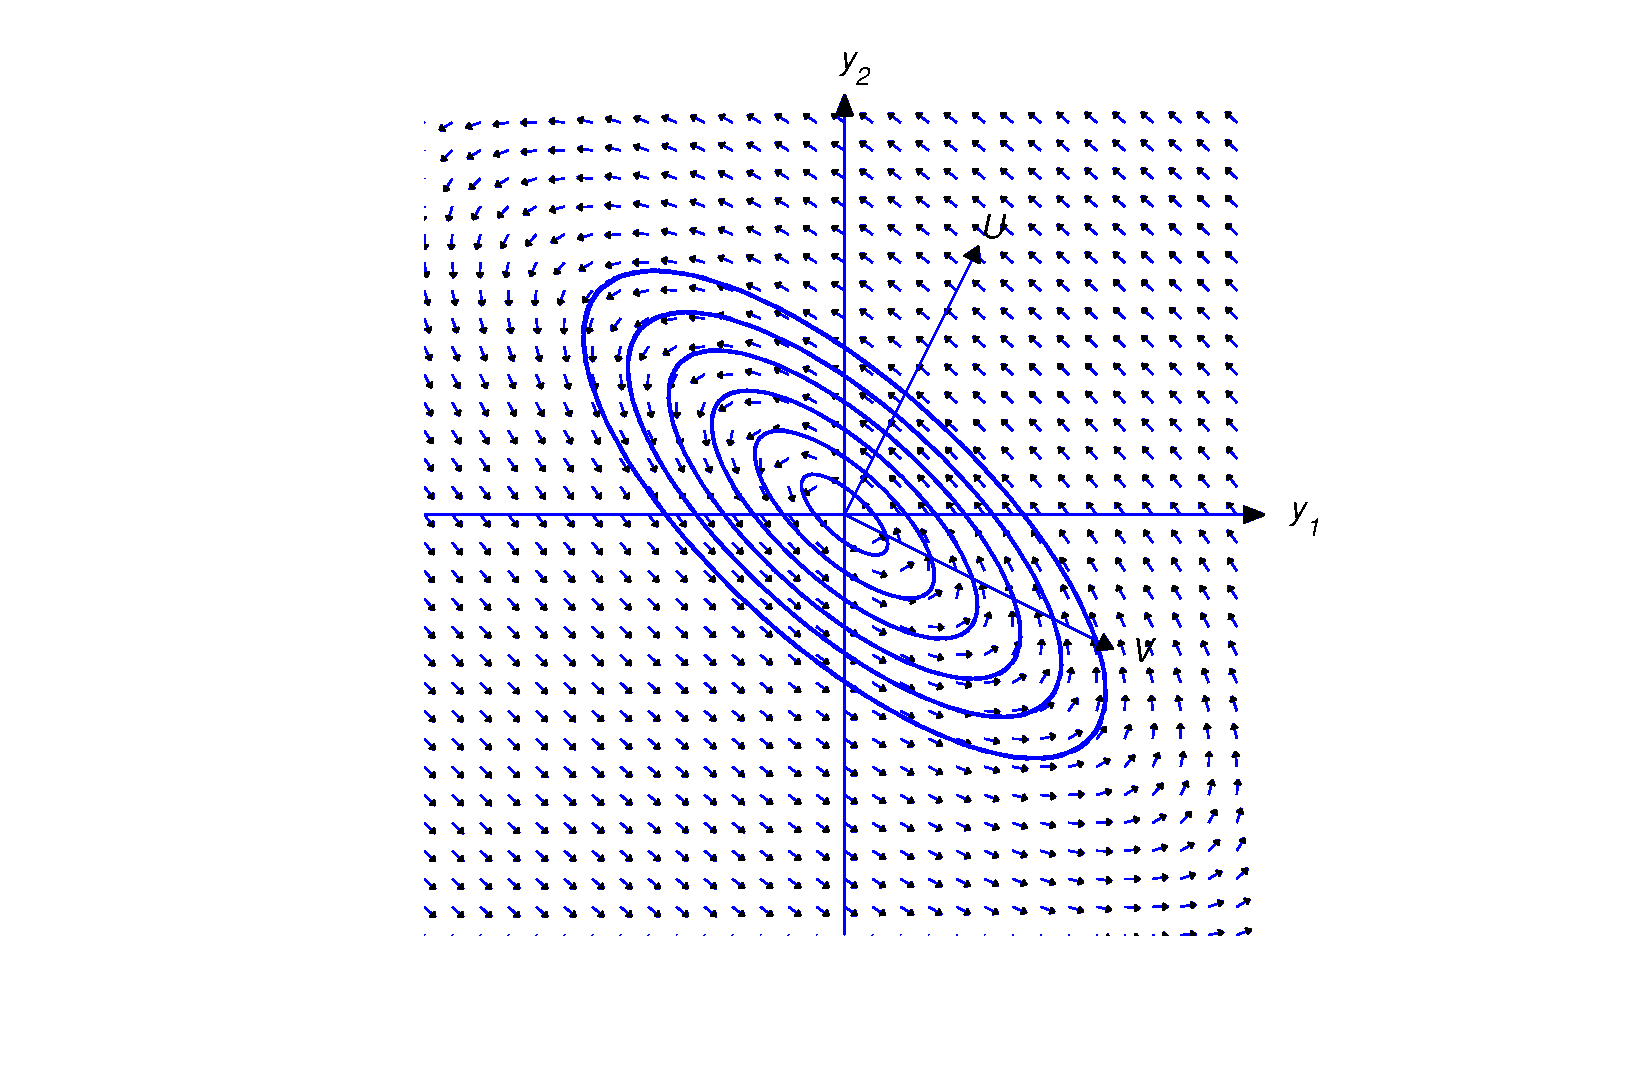
\includegraphics[bb=-78 148 689 643,width=5.67in,height=3.66in,keepaspectratio]{fig100602}}
\caption{ Shadow trajectories traversed counterclockwise}
  \label{figure:10.6.2}
\end{minipage}
\end{figure}

If $\alpha=0$, then any trajectory of \eqref{eq:10.6.10} is a shadow
trajectory of \eqref{eq:10.6.10};  therefore, if $\lambda$ is purely
imaginary, then the trajectories of \eqref{eq:10.6.10} are ellipses
traversed
periodically as indicated in Figures~\ref{figure:10.6.1} and
\ref{figure:10.6.2}.

If $\alpha>0$, then
$$
\lim_{t\to\infty}\|{\bf y}(t)\|=\infty\mbox{\quad and \quad}
\lim_{t\to-\infty}{\bf y}(t)=0,
$$
so the trajectory spirals away from the origin as $t$ varies from
$-\infty$ to $\infty$. The direction of the spiral depends upon the
relative orientation of ${\bf U}$ and ${\bf V}$, as shown in
Figures~\ref{figure:10.6.3} and \ref{figure:10.6.4}.

If $\alpha<0$,  then
$$
\lim_{t\to-\infty}\|{\bf y}(t)\|=\infty\mbox{\quad and \quad}
\lim_{t\to\infty}{\bf y}(t)=0,
$$
\enlargethispage{2in}
so the trajectory spirals toward the origin as $t$ varies from
$-\infty$ to $\infty$. Again, the direction of the spiral depends upon
the relative orientation of ${\bf U}$ and ${\bf V}$, as shown in
Figures~\ref{figure:10.6.5} and \ref{figure:10.6.6}.
\newpage

\begin{figure}[H]
\color{blue}
  \begin{minipage}[b]{0.5\linewidth}
    \centering
   \scalebox{.65}{
  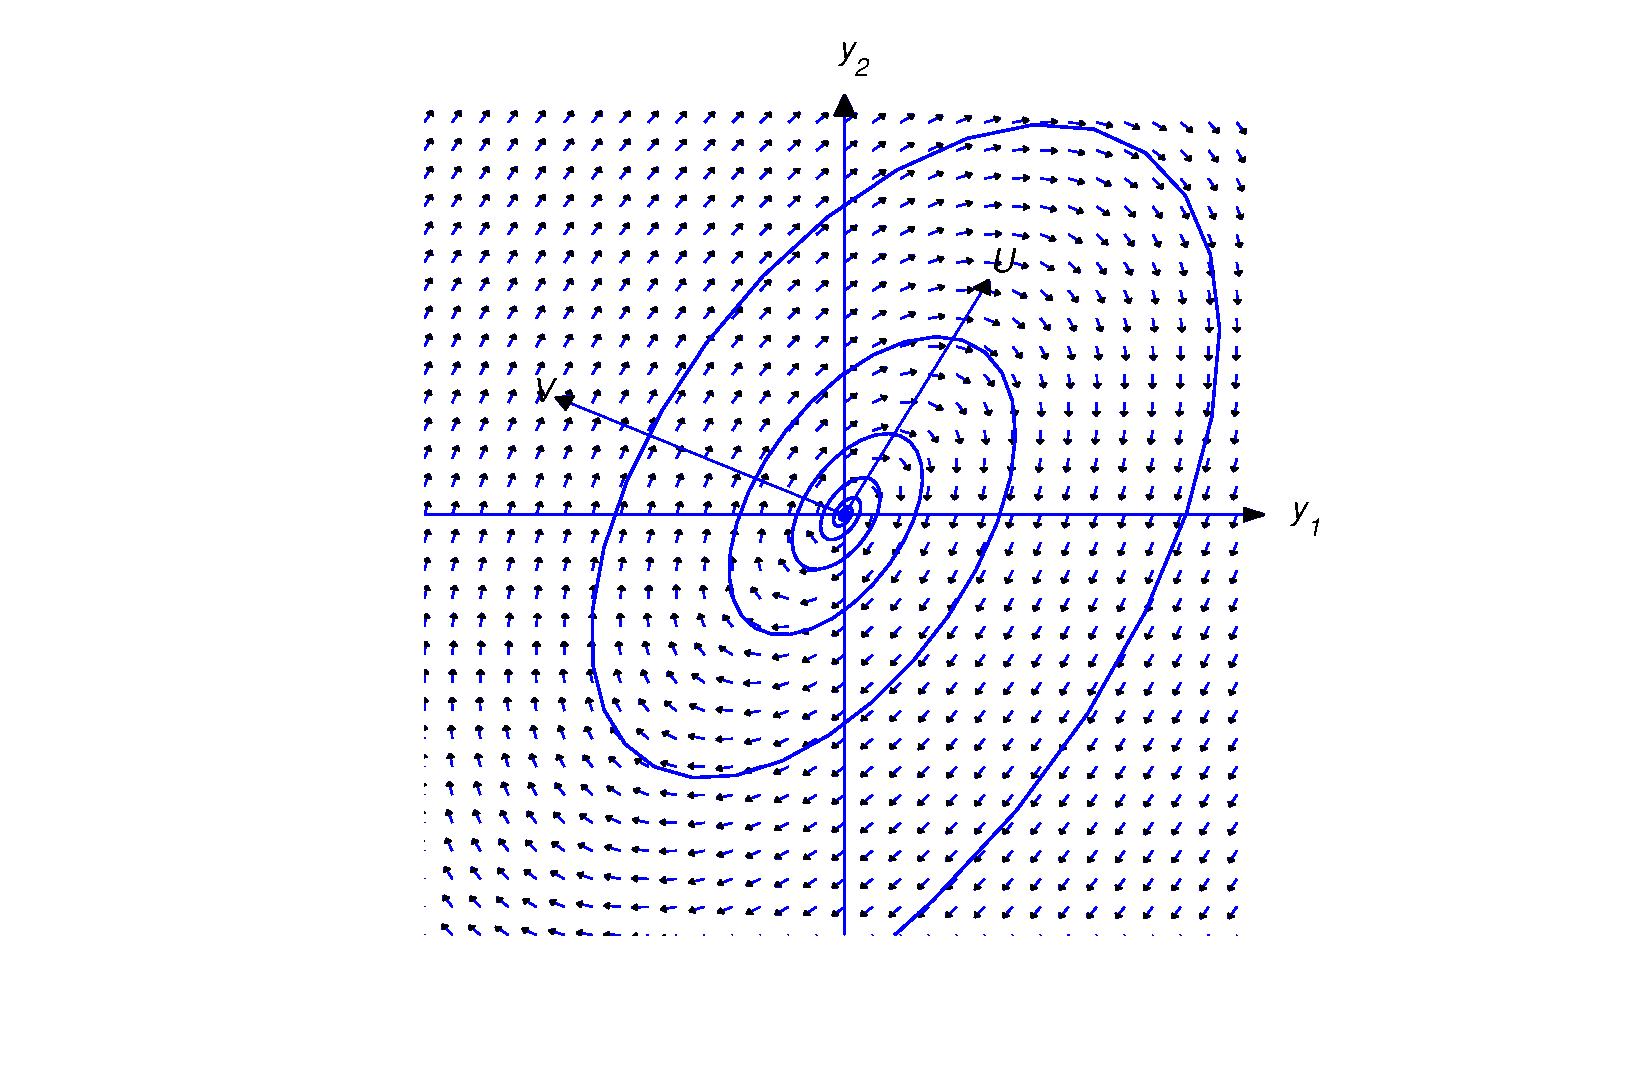
\includegraphics[bb=-78 148 689 643,width=5.67in,height=3.66in,keepaspectratio]{fig010603}}
\caption{ $\alpha>0$;   shadow trajectory spiraling outward}
  \label{figure:10.6.3}
\end{minipage}
  \begin{minipage}[b]{0.5\linewidth}
    \centering
   \scalebox{.65}{
  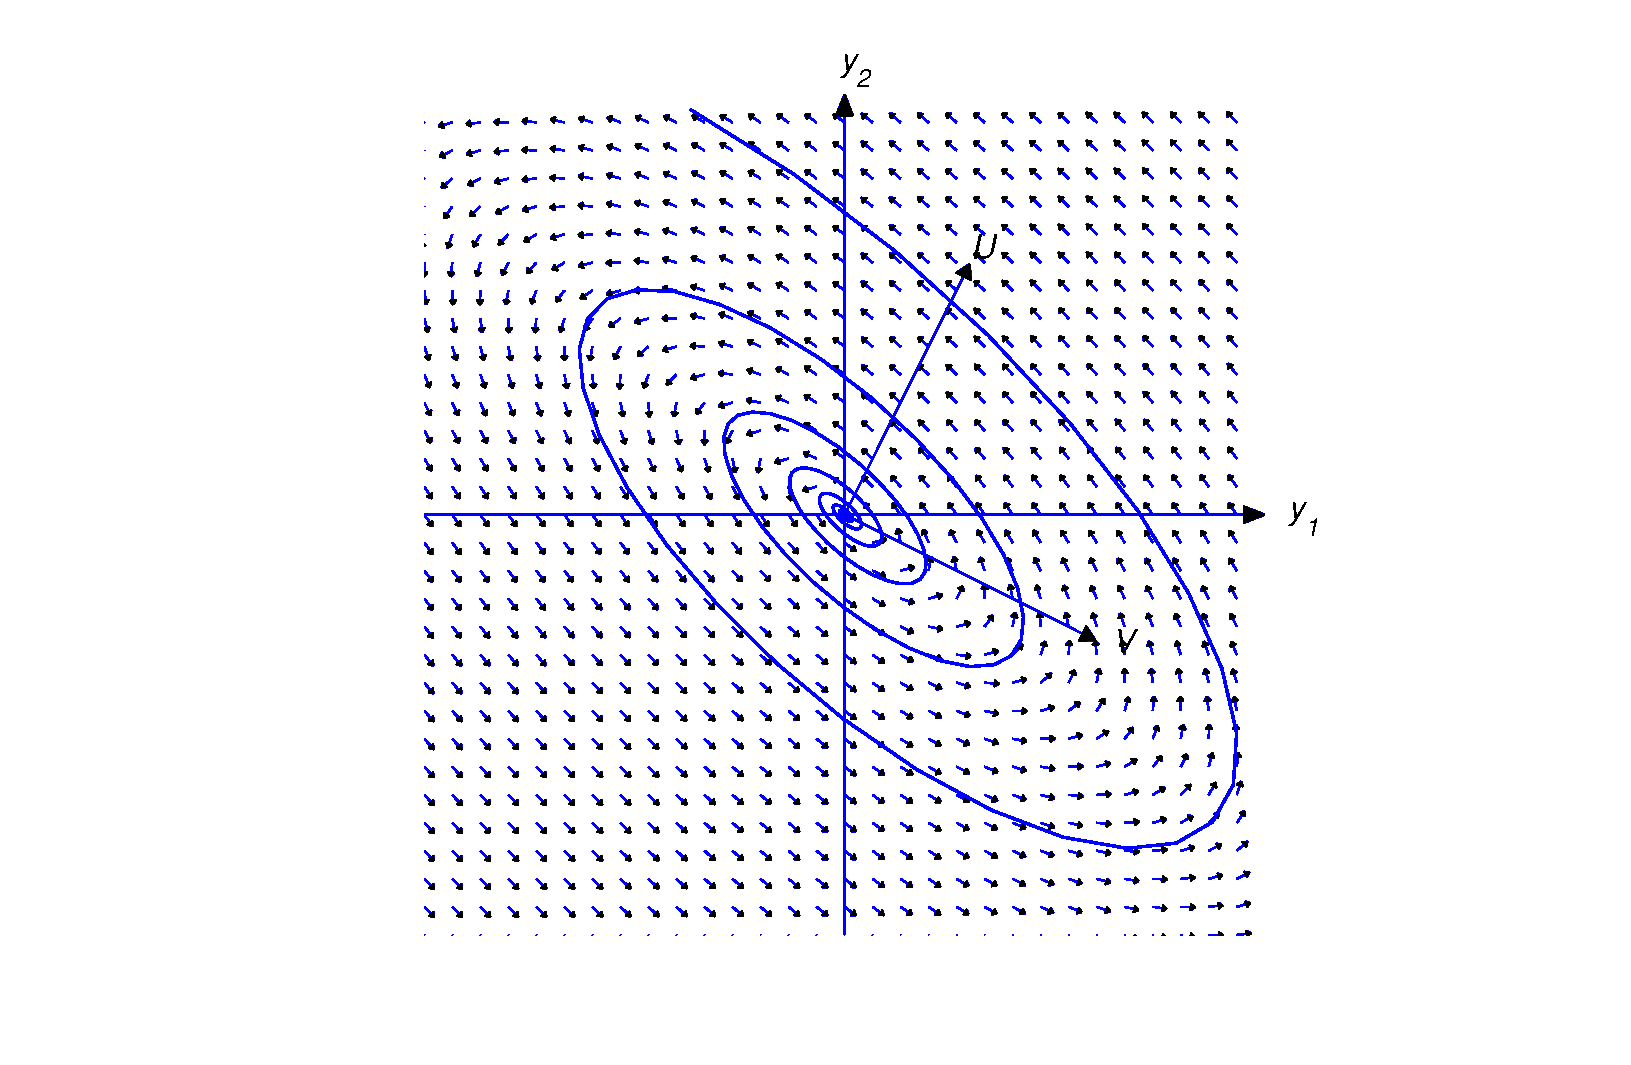
\includegraphics[bb=-78 148 689 643,width=5.67in,height=3.66in,keepaspectratio]{fig010604}}
\caption{ $\alpha>0$;   shadow trajectory spiraling outward}
  \label{figure:10.6.4}
\end{minipage}
\end{figure}

\begin{figure}[H]
\color{blue}
  \begin{minipage}[b]{0.5\linewidth}
    \centering
   \scalebox{.65}{
  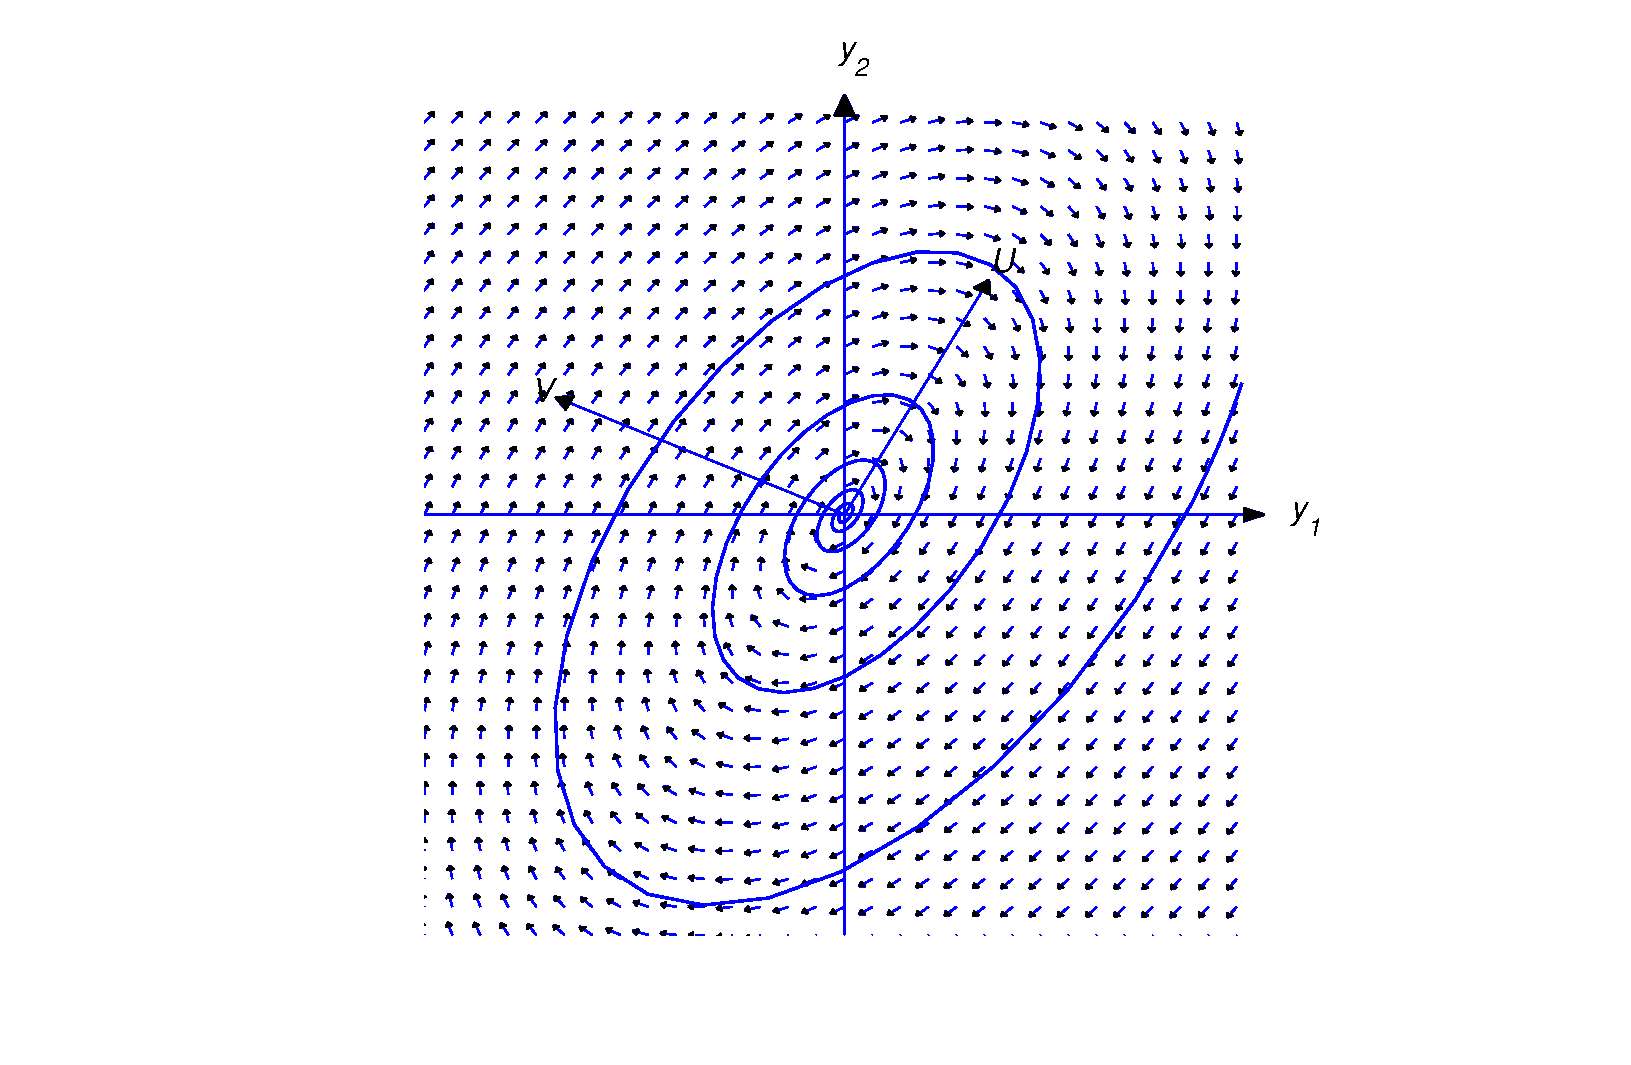
\includegraphics[bb=-78 148 689 643,width=5.67in,height=3.66in,keepaspectratio]{fig010605}}
\caption{ $\alpha<0$;   shadow trajectory spiraling inward}
  \label{figure:10.6.5}
\end{minipage}
  \begin{minipage}[b]{0.5\linewidth}
    \centering
   \scalebox{.65}{
  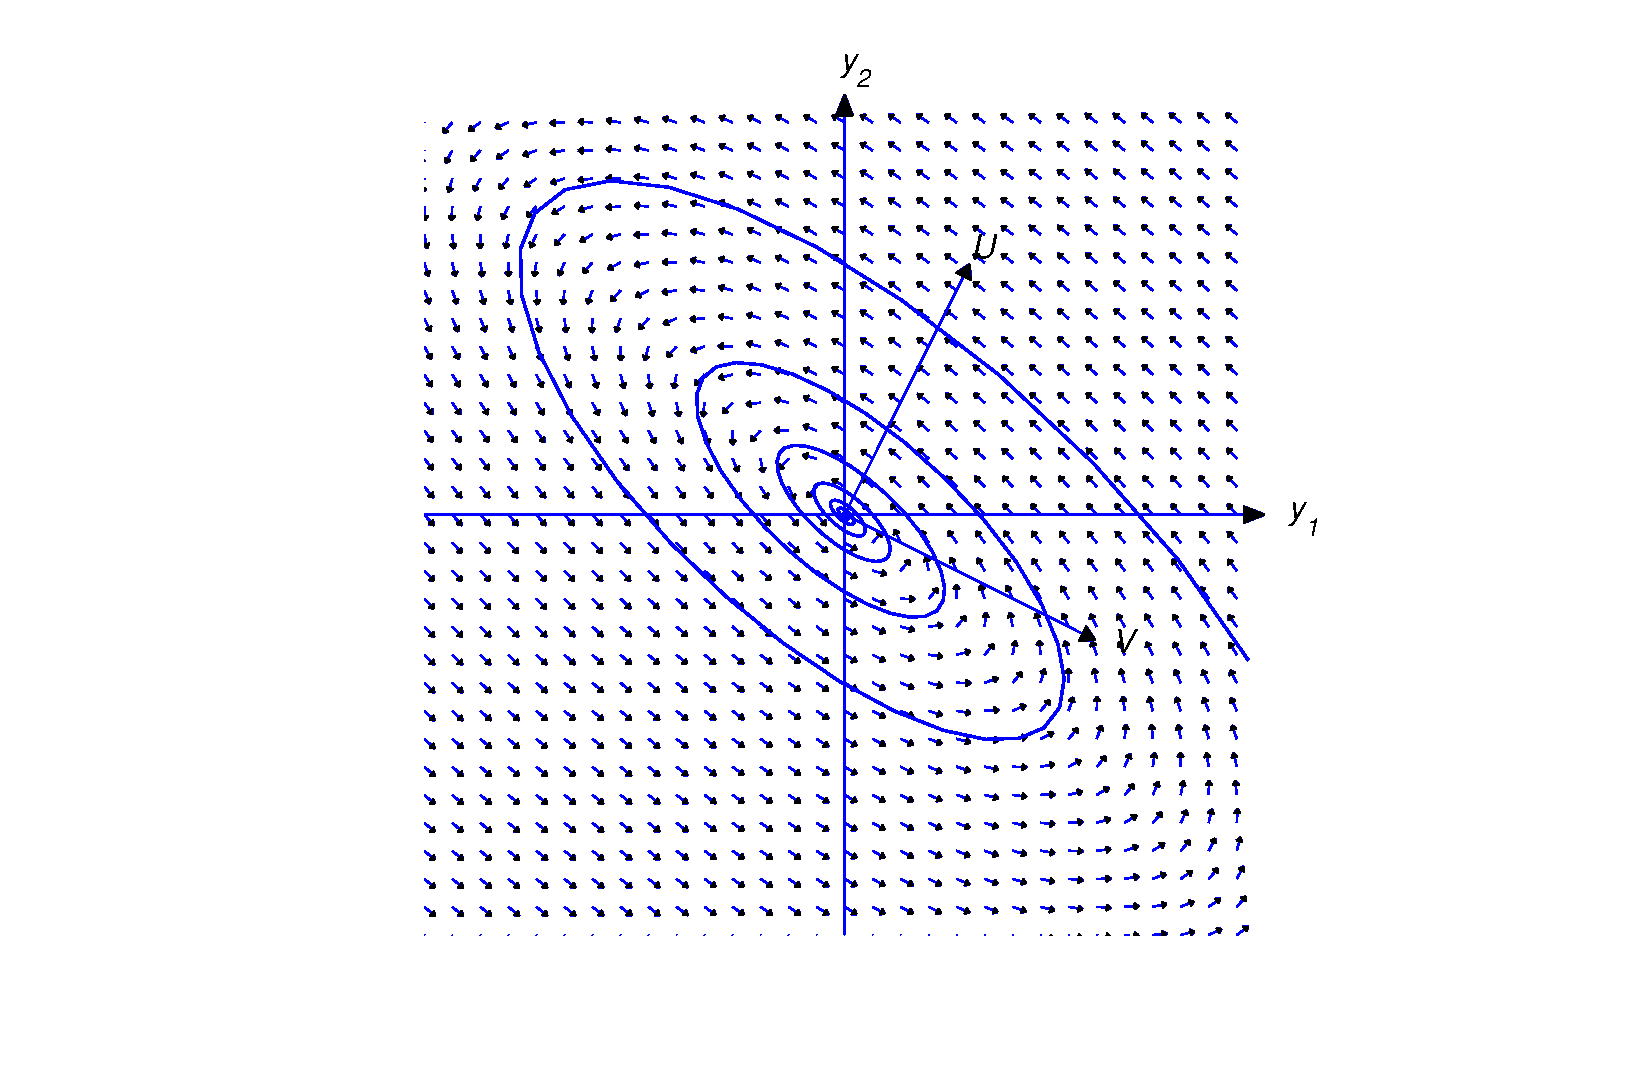
\includegraphics[bb=-78 148 689 643,width=5.67in,height=3.66in,keepaspectratio]{fig100606}}
\caption{ $\alpha<0$;   shadow trajectory spiraling inward}
  \label{figure:10.6.6}
\end{minipage}
\end{figure}

\exercises
In Exercises~\ref{exer:10.6.1}--\ref{exer:10.6.16}  find the general
solution.

\begin{exerciselist}
\begin{tabular}[t]{@{}p{168pt}@{}p{168pt}}
\item\label{exer:10.6.1}  $\dst{{\bf y}'=\twobytwo{-1}2{-5}5{\bf y}
}$&
\item\label{exer:10.6.2}  $\dst{{\bf y}'=\twobytwo{-11}4{-26}9{\bf y}
}$
\end{tabular}

\begin{tabular}[t]{@{}p{168pt}@{}p{168pt}}
\item\label{exer:10.6.3}  $\dst{{\bf y}'=\twobytwo12{-4}5{\bf y}}$&
\item\label{exer:10.6.4}  $\dst{{\bf y}'=\twobytwo5{-6}3{-1}{\bf y}}$
\end{tabular}

\begin{tabular}[t]{@{}p{168pt}@{}p{168pt}}
\item\label{exer:10.6.5}  $\dst{{\bf
y}'=\threebythree3{-3}1022511{\bf y}}$&
\item\label{exer:10.6.6}  $\dst{{\bf
y}'=\threebythree{-3}311{-5}{-3}{-3}73{\bf y}}$
\end{tabular}

\begin{tabular}[t]{@{}p{168pt}@{}p{168pt}}
\item\label{exer:10.6.7} $\dst{{\bf
y}'=\threebythree21{-1}011101{\bf y}}$&
\item\label{exer:10.6.8} $\dst{{\bf
y}'=\threebythree{-3}1{-3}4{-1}24{-2}3{\bf y}}$
\end{tabular}

\begin{tabular}[t]{@{}p{168pt}@{}p{168pt}}
\item\label{exer:10.6.9}  $\dst{{\bf y}'=\twobytwo5{-4}{10}1{\bf
y}}$&
 \item\label{exer:10.6.10}  $\dst{{\bf
y}'={1\over3}\twobytwo7{-5}25{\bf y}}$
\end{tabular}

\begin{tabular}[t]{@{}p{168pt}@{}p{168pt}}
\item\label{exer:10.6.11}  $\dst{{\bf y}'=\twobytwo32{-5}1{\bf y}}$&
\item\label{exer:10.6.12}  $\dst{{\bf
y}'=\twobytwo{34}{52}{-20}{-30}{\bf y}}$
\end{tabular}

\begin{tabular}[t]{@{}p{168pt}@{}p{168pt}}
\item\label{exer:10.6.13}  $\dst{{\bf y}'
=\threebythree11210{-1}{-1}{-2}{-1}{\bf y}}$&
\item\label{exer:10.6.14}  $\dst{{\bf y}'
=\threebythree3{-4}{-2}{-5}7{-8}{-10}{13}{-8}{\bf y}}$
\end{tabular}

\begin{tabular}[t]{@{}p{168pt}@{}p{168pt}}
\item\label{exer:10.6.15}  $\dst{{\bf
y}'=\threebythree60{-3}{-3}331{-2}6{\bf y}'}$&
\item\label{exer:10.6.16}  $\dst{{\bf
y}'=\threebythree12{-2}02{-1}100{\bf y}'}$
\end{tabular}

\exercisetext{In Exercises~\ref{exer:10.6.17}--\ref{exer:10.6.24}
solve the initial value problem.}

\item\label{exer:10.6.17}
$\dst{{\bf y}'=\twobytwo4{-6}3{-2}{\bf y},\quad {\bf
y}(0)=\twocol52}$

\item\label{exer:10.6.18}
$\dst{{\bf y}'=\twobytwo7{15}{-3}1{\bf y},\quad {\bf
y}(0)=\twocol51}$

\item\label{exer:10.6.19}
$\dst{{\bf y}'=\twobytwo7{-15}3{-5}{\bf y},\quad {\bf
y}(0)=\twocol{17}7}$

\item\label{exer:10.6.20}
$\dst{{\bf y}'={1\over6}\twobytwo4{-2}52{\bf y},\quad {\bf
y}(0)=\twocol1{-1}}$

\item\label{exer:10.6.21}
$\dst{{\bf y}'=\threebythree52{-1}{-3}22132{\bf y},\quad {\bf
y}(0)=\threecol406}$

\item\label{exer:10.6.22}
$\dst{{\bf y}'=\threebythree4408{10}{-20}23{-2}{\bf y},\quad {\bf
y}(0)=\threecol865}$

\item\label{exer:10.6.23}
$\dst{{\bf
y}'=\threebythree1{15}{-15}{-6}{18}{-22}{-3}{11}{-15}{\bf
y},\quad {\bf y}(0)=\threecol{15}{17}{10}}$

\item\label{exer:10.6.24}
$\dst{{\bf y}'=\threebythree4{-4}4{-10}3{15}2{-3}1{\bf y},\quad
{\bf y}(0)=\threecol{16}{14}6}$

\item\label{exer:10.6.25}
Suppose an $n\times n$ matrix $A$ with
real entries has a complex eigenvalue $\lambda=\alpha+i\beta$
($\beta\ne0$) with associated eigenvector ${\bf x}={\bf u}+i{\bf v}$,
where ${\bf u}$ and ${\bf v}$ have real components. Show that ${\bf
u}$ and ${\bf v}$ are both nonzero.

\item\label{exer:10.6.26}
Verify that
$$
{\bf y}_1=e^{\alpha t}({\bf u}\cos\beta t-{\bf v}\sin\beta t)
\mbox{\quad and\quad}
{\bf y}_2=e^{\alpha t}({\bf u}\sin\beta t+{\bf v}\cos\beta t),
$$
are the real and imaginary parts of
$$
e^{\alpha t}(\cos\beta t+i\sin\beta t)({\bf u}+i{\bf v}).
$$

\item\label{exer:10.6.27}
 Show that if the vectors ${\bf u}$ and ${\bf v}$ are not both ${\bf
0}$ and $\beta\ne0$ then the vector functions
$$
{\bf y}_1=e^{\alpha t}({\bf u}\cos\beta t-{\bf v}\sin\beta t)\quad
\mbox{ and }\quad
{\bf y}_2=e^{\alpha t}({\bf u}\sin\beta t+{\bf v}\cos\beta t)
$$
are linearly independent on every interval. \hint{There are
two
cases to consider: {\rm(i)} $\{{\bf u},{\bf v}\}$ linearly
independent, and {\rm(ii)}
 $\{{\bf u},{\bf v}\}$ linearly dependent. In either case, exploit the linear independence of $\{\cos\beta t,\sin\beta t\}$
on every interval.}

\item\label{exer:10.6.28}
Suppose ${\bf u}=\dst{\twocol{u_1}{u_2}}$ and ${\bf
v}=\dst{\twocol{v_1}{v_2}}$ are not orthogonal; that is, $({\bf
u},{\bf v})\ne0$.
\begin{alist}
\item % (a)
Show that  the quadratic equation
$$
({\bf u},{\bf v})k^2+(\|{\bf v}\|^2-\|{\bf u}\|^2)k-({\bf u},{\bf
v})=0
$$
has a positive root $k_1$ and a negative root $k_2=-1/k_1$.
\item % (b)
Let ${\bf u}_1^{(1)}={\bf u}-k_1{\bf v}$, ${\bf v}_1^{(1)}={\bf
v}+k_1{\bf u}$, ${\bf u}_1^{(2)}={\bf u}-k_2{\bf v}$, and ${\bf
v}_1^{(2)}={\bf v}+k_2{\bf u}$, so that $({\bf u}_1^{(1)},{\bf
v}_1^{(1)}) =({\bf u}_1^{(2)},{\bf v}_1^{(2)})=0$, from the discussion
given above. Show that
$$
{\bf u}_1^{(2)}={{\bf v}_1^{(1)}\over k_1}
\mbox{\quad and \quad}
{\bf v}_1^{(2)}=-{{\bf u}_1^{(1)}\over k_1}.
$$
\item % (c)
Let ${\bf U}_1$, ${\bf V}_1$, ${\bf U}_2$, and ${\bf V}_2$ be unit
vectors in the directions of ${\bf u}_1^{(1)}$, ${\bf v}_1^{(1)}$,
${\bf u}_1^{(2)}$, and ${\bf v}_1^{(2)}$, respectively. Conclude from
\part{a} that ${\bf U}_2={\bf V}_1$ and ${\bf V}_2=-{\bf U}_1$, and
that therefore the counterclockwise angles from ${\bf U}_1$ to ${\bf
V}_1$ and from ${\bf U}_2$ to ${\bf V}_2$ are both $\pi/2$ or both
$-\pi/2$.
\end{alist}

\exercisetext{In Exercises~\ref{exer:10.6.29}-\ref{exer:10.6.32} find vectors
${\bf U}$ and ${\bf V}$ parallel to the axes of symmetry of the
trajectories, and plot some typical trajectories.}

\begin{tabular}[t]{@{}p{168pt}@{}p{168pt}}
\item\label{exer:10.6.29} \CGex\, $\dst{{\bf y}'=\twobytwo3{-5}5{-3}{\bf
y}}$&
\item\label{exer:10.6.30} \CGex\,  $\dst{{\bf y}'=\twobytwo{-15}{10}{-25}{15}{\bf y}}$
\end{tabular}

\begin{tabular}[t]{@{}p{168pt}@{}p{168pt}}
\item\label{exer:10.6.31} \CGex\,  $\dst{{\bf y}'=\twobytwo{-4}8{-4}4{\bf y}}$&
\item\label{exer:10.6.32} \CGex\,  $\dst{{\bf y}'=\twobytwo{-3}{-15}33{\bf y}}$
\end{tabular}

\exercisetext{In Exercises~\ref{exer:10.6.33}-\ref{exer:10.6.40} find vectors
${\bf U}$ and ${\bf V}$ parallel to the axes of symmetry of the shadow
trajectories, and plot a typical trajectory.}

\begin{tabular}[t]{@{}p{168pt}@{}p{168pt}}
\item\label{exer:10.6.33} \CGex\,  $\dst{{\bf y}'=\twobytwo{-5}6{-12}7{\bf y}}$&
\item\label{exer:10.6.34} \CGex\,  $\dst{{\bf y}'=\twobytwo5{-12}6{-7}{\bf y}}$
\end{tabular}

\begin{tabular}[t]{@{}p{168pt}@{}p{168pt}}
\item\label{exer:10.6.35} \CGex\,  $\dst{{\bf y}'=\twobytwo4{-5}9{-2}{\bf y}}$&
\item\label{exer:10.6.36} \CGex\,  $\dst{{\bf y}'=\twobytwo{-4}9{-5}2{\bf y}}$
\end{tabular}

\begin{tabular}[t]{@{}p{168pt}@{}p{168pt}}
\item\label{exer:10.6.37} \CGex\,  $\dst{{\bf y}'=\twobytwo{-1}{10}{-10}{-1}{\bf y}}$&
\item\label{exer:10.6.38} \CGex\,  $\dst{{\bf y}'=\twobytwo{-1}{-5}{20}{-1}{\bf y}}$
\end{tabular}

\enlargethispage{1in}
\begin{tabular}[t]{@{}p{168pt}@{}p{168pt}}
\item\label{exer:10.6.39} \CGex\,  $\dst{{\bf y}'=\twobytwo{-7}{10}{-10}9{\bf y}}$&
\item\label{exer:10.6.40} \CGex\,  $\dst{{\bf y}'=\twobytwo{-7}6{-12}5{\bf y}}$
\end{tabular}

\end{exerciselist}


\section{Variation of Parameters for Nonhomogeneous Linear Systems}

\noindent
We now consider the nonhomogeneous linear system
$$
{\bf y}'= A(t){\bf y}+{\bf f}(t),
$$
where $A$ is an $n\times n$ matrix function and ${\bf f}$ is an
$n$-vector forcing function. Associated with this system is the {\color{blue}\it
complementary system\/} ${\bf y}'=A(t){\bf y}$.

The next theorem is analogous to
Theorems~\ref{thmtype:5.3.2} and
\ref{thmtype:9.1.5}. It shows how to find the general solution
of
${\bf y}'=A(t){\bf y}+{\bf f}(t)$ if we know a particular solution of ${\bf
y}'=A(t){\bf y}+{\bf f}(t)$ and a fundamental set of solutions of the
complementary system. We leave the proof as an exercise
(Exercise~\ref{exer:10.7.21}).

\begin{theorem}\color{blue}\label{thmtype:10.7.1}
Suppose the $n\times n$ matrix function $A$ and the $n$-vector
function ${\bf f}$ are continuous on $(a,b).$ Let ${\bf y}_p$ be a
particular solution of ${\bf y}'=A(t){\bf y}+{\bf f}(t)$ on $(a,b)$,
and let
$\{{\bf y}_1,{\bf y}_2,\dots,{\bf y}_n\}$ be a fundamental set of
solutions of the complementary equation ${\bf y}'=A(t){\bf y}$ on
$(a,b)$. Then ${\bf y}$ is a solution of ${\bf y}'=A(t){\bf y}+{\bf
f}(t)$ on $(a,b)$ if and only if
$$
{\bf y}={\bf y}_p+c_1{\bf y}_1+c_2{\bf y}_2+\cdots+c_n{\bf y}_n,
$$
where $c_1,$ $c_2,$ \dots, $c_n$  are constants.
\end{theorem}

\boxit{Finding a Particular Solution of a Nonhomogeneous System}

\noindent
We now discuss an extension of the method of variation of parameters
to linear nonhomogeneous systems. This method will produce a
particular solution of a nonhomogeneous system ${\bf y}'=A(t){\bf
y}+{\bf f}(t)$ provided that we know a fundamental matrix for the
complementary system. To derive the method, suppose $Y$ is a
fundamental matrix for the complementary system; that is,
$$
Y=\left[\begin{array}{cccc}
y_{11}&y_{12}&\cdots&y_{1n} \\
y_{21}&y_{22}&\cdots&y_{2n}\\
\vdots&\vdots&\ddots&\vdots \\
y_{n1}&y_{n2}&\cdots&y_{nn} \\
\end{array} \right],
$$
where
$$
{\bf y}_1=\left[\begin{array}{c}y_{11}\\y_{21}\\ \vdots\\
y_{n1}\end{array}\right],\quad
{\bf y}_2=\left[\begin{array}{c}y_{12}\\y_{22}\\ \vdots\\
y_{n2}\end{array}\right],\quad \cdots,\quad
{\bf y}_n=\left[\begin{array}{c}y_{1n}\\y_{2n}\\ \vdots\\
y_{nn}\end{array}\right]
$$
is a fundamental set of solutions of the complementary system.
In Section~10.3 we saw that $Y'=A(t)Y$. We seek a
particular solution of
\begin{equation} \label{eq:10.7.1}
{\bf y}'=A(t){\bf y}+{\bf f}(t)
\end{equation}
 of the form
\begin{equation} \label{eq:10.7.2}
{\bf y}_p=Y{\bf u},
\end{equation}
 where ${\bf u}$ is to be determined. Differentiating \eqref{eq:10.7.2} yields
\begin{eqnarray*}
 {\bf y}_p'&=&Y' {\bf u}+Y {\bf u}'
\\&=&A Y {\bf u}+Y {\bf u}'\mbox{ (since $Y'=AY$)}\\&=&
 A{\bf y}_p+Y {\bf u}'\mbox{ (since $Y{\bf u}={\bf y}_p$)}.
\end{eqnarray*}
Comparing this with  \eqref{eq:10.7.1} shows that ${\bf y}_p=Y{\bf u}$ is a
solution of \eqref{eq:10.7.1} if and only if
$$
Y{\bf u}'={\bf f}.
$$
Thus, we can find a particular solution ${\bf y}_p$ by solving this
equation for ${\bf u}'$, integrating to obtain ${\bf u}$, and
computing $Y{\bf u}$. We can take all constants of integration to be
zero, since any particular solution will suffice.

Exercise~\ref{exer:10.7.22} sketches a proof that this method is analogous
to the method of variation of parameters discussed in
Sections~5.7 and 9.4 for scalar linear
equations.

\begin{example}\label{example:10.7.1} \rm \mbox{}\newline
\begin{alist}
\item % (a)
Find a particular solution of the system
\begin{equation} \label{eq:10.7.3}
{\bf y}'=\twobytwo1221{\bf y}+\left[\begin{array}{c}2e^{4t}\\e^{4t}
\end{array}\right],
\end{equation}
which we considered in Example~\ref{example:10.2.1}.
\item % (b)
Find the general solution of  \eqref{eq:10.7.3}.
\end{alist}
\end{example}

\solutionpart{a}   The complementary system is
\begin{equation} \label{eq:10.7.4}
{\bf y}'=\twobytwo1221{\bf y}.
\end{equation}
The characteristic polynomial of the coefficient matrix is
$$
\left|\begin{array}{cc}1-\lambda&2\\2&1-\lambda\end{array}\right|=
(\lambda+1)(\lambda-3).
$$
Using the method of Section~10.4, we find that
$$
{\bf y}_1=\left[\begin{array}{r}e^{3t}\\e^{3t}\end{array}\right]
\mbox{\quad and \quad}
{\bf y}_2=\left[\begin{array}{r}e^{-t}\\-e^{-t}\end{array}\right]
$$
are linearly independent solutions of \eqref{eq:10.7.4}.
Therefore
$$
Y=\left[\begin{array}{rr}e^{3t}&e^{-t}\\e^{3t}&-e^{-t}\end{array}\right]
$$
is a fundamental matrix for \eqref{eq:10.7.4}. We seek a particular
solution ${\bf y}_p=Y{\bf u}$ of \eqref{eq:10.7.3}, where $Y{\bf u}'={\bf
f}$; that is,
$$
\left[\begin{array}{rr}e^{3t}&e^{-t}\\e^{3t}&-e^{-t}\end{array}\right]
\twocol{u_1'}{u_2'}
=\left[\begin{array}{c}2e^{4t}\\e^{4t}\end{array}\right].
$$
The determinant of $Y$ is the Wronskian
$$
\left|\begin{array}{rr}e^{3t}&e^{-t}\\e^{3t}&-e^{-t}\end{array}\right|
=-2e^{2t}.
$$
By Cramer's rule,
$$
\begin{array}{ccccccl}
u_1'&=&-\dst{1\over2e^{2t}}
\left|\begin{array}{cr}2e^{4t}&e^{-t}\\e^{4t}&-e^{-t}
\end{array}\right|&=&\dst{3e^{3t}\over2e^{2t}}&=
&\dst{3\over2}e^t,\\[4\jot]
u_2'&=&-\dst{1\over2e^{2t}}
\left|\begin{array}{rr}e^{3t}&2e^{4t}\\e^{3t}&e^{4t}
\end{array}\right|&=&\dst{e^{7t}\over2e^{2t}}&=&\dst{1\over2}e^{5t}.
\end{array}
$$
 Therefore
$$
{\bf
u}'={1\over2}\left[\begin{array}{c}3e^t\\e^{5t}\end{array}\right].
$$
Integrating and taking the constants of integration to be zero yields
$$
{\bf
u}={1\over10}\left[\begin{array}{c}15e^t\\e^{5t}\end{array}\right],
$$
so
$$
{\bf y}_p=Y{\bf u}=
\dst{1\over10}\left[\begin{array}{rr}e^{3t}&e^{-t}\\[2\jot]
e^{3t}&-e^{-t}\end{array}\right]
\left[\begin{array}{c}15e^t\\e^{5t}\end{array}\right]
=\phantom{0}
\dst{1\over5}\left[\begin{array}{c}8e^{4t}\\7e^{4t}\end{array}\right]
$$
is a particular solution of  \eqref{eq:10.7.3}.

\solutionpart{b} From Theorem~\ref{thmtype:10.7.1}, the general solution of
\eqref{eq:10.7.3} is
\begin{equation} \label{eq:10.7.5}
{\bf y}={\bf y}_p+c_1{\bf y}_1+c_2{\bf y}_2=
{1\over5}\left[\begin{array}{c}8e^{4t}\\7e^{4t}\end{array}\right]
+c_1\left[\begin{array}{r}e^{3t}\\e^{3t}\end{array}\right]
+c_2\left[\begin{array}{r}e^{-t}\\-e^{-t}\end{array}\right],
\end{equation}
which can also be written as
$$
{\bf y}=
{1\over5}\left[\begin{array}{c}8e^{4t}\\7e^{4t}\end{array}\right]
+\left[\begin{array}{rr}e^{3t}&e^{-t}\\e^{3t}&-e^{-t}\end{array}\right]
{\bf c},
$$
where ${\bf c}$ is an arbitrary constant vector.

Writing \eqref{eq:10.7.5} in terms of
coordinates yields
\begin{eqnarray*}
y_1&=&{8\over5}e^{4t}+c_1e^{3t}+c_2e^{-t}\\[2\jot]
y_2&=&{7\over5}e^{4t}+c_1e^{3t}-c_2e^{-t},
\end{eqnarray*}
so our result is consistent with Example~\ref{example:10.2.1}.
\bbox.

If $A$ isn't  a constant matrix, it's usually difficult to find a
fundamental set of solutions for the system ${\bf y}'=A(t){\bf y}$. It
is beyond the scope of this text to discuss methods for doing this.
Therefore, in the following examples and in the exercises involving
systems with variable coefficient matrices we'll provide fundamental
matrices for the complementary systems without explaining how they
were obtained.

\begin{example}\label{example:10.7.2} \rm
Find a particular solution of
\begin{equation} \label{eq:10.7.6}
{\bf y}'=\left[\begin{array}{cc}2&2e^{-2t}\\2e^{2t}&4\end{array}\right]{\bf
y}+\twocol11,
\end{equation}
given that
$$
Y=\left[\begin{array}{cc} e^{4t}&-1\\e^{6t}&e^{2t}\end{array}\right]
$$
is  a fundamental matrix for the complementary system.
\end{example}

\solution
We seek a particular solution
${\bf y}_p=Y{\bf u}$ of \eqref{eq:10.7.6} where
 $Y{\bf u}'={\bf f}$; that is,
$$
\left[\begin{array}{cc} e^{4t}&-1\\e^{6t}&e^{2t}\end{array}\right]
\twocol{u_1'}{u_2'}=\twocol11.
$$
The determinant of $Y$ is the Wronskian
$$
\left|\begin{array}{cc}
e^{4t}&-1\\e^{6t}&e^{2t}\end{array}\right|=2e^{6t}.
$$
By Cramer's rule,
$$
\begin{array}{cccccll}
u_1'&=&\dst{1\over2e^{6t}}\left|\begin{array}{cc}1&-1\\1&e^{2t}
\end{array}\right|&=&\dst{e^{2t}+1\over2e^{6t}}&=&\dst{e^{-4t}+e^{-6t}\over2}
\\[4\jot]
u_2'&=&\dst{1\over2e^{6t}}\left|\begin{array}{cc}e^{4t}&1\\e^{6t}&1
\end{array}\right|&=&\dst{e^{4t}-e^{6t}\over2e^{6t}}&=&\dst{e^{-2t}-1\over2}.
\end{array}
$$
Therefore
$$
{\bf
u}'={1\over2}\left[\begin{array}{c}e^{-4t}+e^{-6t}\\e^{-2t}-1\end{array}\right].
$$
Integrating  and taking the constants of integration to be zero yields
$$
{\bf
u}=-{1\over24}\left[\begin{array}{c}3e^{-4t}+2e^{-6t}\\6e^{-2t}+12t
\end{array}\right],
$$
so
$$
{\bf y}_p=Y{\bf u}=
-\displaystyle{1\over24}\left[\begin{array}{cc}e^{4t}&-1\\e^{6t}&e^{2t}\end{array}\right]
\left[\begin{array}{c}3e^{-4t}+2e^{-6t}\\6e^{-2t}+12t\end{array}\right]
=\displaystyle{1\over24}\left[\begin{array}{c}4e^{-2t}+12t-3\\-3e^{2t}(4t+1)-8\end{array}\right]
$$
is a particular solution of  \eqref{eq:10.7.6}.

\begin{example}\label{example:10.7.3} \rm
Find a particular solution of
\begin{equation} \label{eq:10.7.7}
{\bf y}'=-{2\over t^2
}\left[\begin{array}{cc}t&-3t^2\\1&-2t\end{array}\right]{\bf y}
+t^2\twocol11,
\end{equation}
given that
$$
Y=\left[\begin{array}{cc}2t&3t^2\\1&2t\end{array}\right]
$$
is a fundamental matrix for the complementary system on $(-\infty,0)$
and $(0,\infty)$.
\end{example}

\solution
We seek a particular solution ${\bf y}_p=Y{\bf u}$ of \eqref{eq:10.7.7}
where $Y{\bf u}'={\bf f}$; that is,
$$
\left[\begin{array}{cc}2t&3t^2\\1&2t\end{array}\right]\twocol{u_1'}{u_2'}
=\twocol{t^2}{t^2}.
$$
The determinant of $Y$  is the Wronskian
$$
\left|\begin{array}{cc}2t&3t^2\\1&2t\end{array}\right|=t^2.
$$
By Cramer's rule,
$$
\begin{array}{ccccccl}
u_1'&=&\dst{1\over t^2}\left|\begin{array}{cc}t^2&3t^2\\t^2&2t
\end{array}\right|&=&\dst{2t^3-3t^4\over t^2}&=&2t-3t^2,
\\[4\jot]
u_2'&=&\dst{1\over t^2}\left|\begin{array}{cc}2t&t^2\\1&t^2
\end{array}\right|&=&\dst{2t^3-t^2\over t^2}&=&2t-1.
\end{array}
$$
Therefore
$$
{\bf
u}'=\left[\begin{array}{c}2t-3t^2\\2t-1\end{array}\right].
$$
Integrating  and taking the constants of integration to be zero yields
$$
{\bf
u}=\left[\begin{array}{c}t^2-t^3\\t^2-t
\end{array}\right],
$$
so
$$
{\bf y}_p=Y{\bf u}=
\left[\begin{array}{cc}2t&3t^2\\1&2t\end{array}\right]
\left[\begin{array}{c}t^2-t^3\\t^2-t\end{array}\right]
=\left[\begin{array}{c}t^3(t-1)\\t^2(t-1)\end{array}\right]
$$
is a particular solution of  \eqref{eq:10.7.7}.

\begin{example}\label{example:10.7.4} \rm \mbox{}\newline
\begin{alist}
\item % (a)
Find a particular solution of
\begin{equation} \label{eq:10.7.8}
{\bf y}'=\threebythree2{-1}{-1}10{-1}1{-1}0{\bf
y}+\left[\begin{array}{c}e^{t}\\0\\e^{-t}
\end{array}\right].
\end{equation}
\item % (b)
Find the general solution of  \eqref{eq:10.7.8}.
\end{alist}
\end{example}

\solutionpart{a} The complementary system for \eqref{eq:10.7.8} is
\begin{equation} \label{eq:10.7.9}
{\bf y}'=\threebythree2{-1}{-1}10{-1}1{-1}0{\bf y}.
\end{equation}
The characteristic polynomial of the coefficient matrix is
$$
\left|\begin{array}{ccc}2-\lambda&-1&-1\\1&-\lambda&-1\\1&-1&-\lambda
\end{array}\right|=
-\lambda(\lambda-1)^2.
$$
Using the method of Section~10.4, we find that
$$
{\bf y}_1=\left[\begin{array}{c}1\\1\\1\end{array}\right],\quad
{\bf y}_2=\left[\begin{array}{c}e^t\\e^t\\0\end{array}\right],
\mbox{\quad and \quad}
{\bf y}_3=\left[\begin{array}{c}e^t\\0\\e^t\end{array}\right]
$$
are linearly independent solutions of \eqref{eq:10.7.9}.
Therefore
$$
Y=\left[\begin{array}{ccc}1&e^t&e^t\\1&e^t&0\\1&0&e^t\end{array}\right]
$$
is a fundamental matrix for  \eqref{eq:10.7.9}.
We seek a particular solution  ${\bf y}_p=Y{\bf u}$ of
\eqref{eq:10.7.8}, where
$Y{\bf u}'={\bf f}$; that is,
$$
\left[\begin{array}{ccc}1&e^t&e^t\\1&e^t&0\\1&0&e^t\end{array}\right]
\threecol{u_1'}{u_2'}{u_3'}=
\left[\begin{array}{c}e^t\\0\\e^{-t}\end{array}\right].
$$
The determinant of $Y$  is the Wronskian
$$
\left|\begin{array}{ccc}1&e^t&e^t\\1&e^t&0\\1&0&e^t\end{array}\right|
=-e^{2t}.
$$
Thus, by Cramer's rule,
$$
\begin{array}{cccccll}
u_1'&=&-\dst{1\over
e^{2t}}\left|\begin{array}{ccc}e^t&e^t&e^t\\0&e^t&0\\e^{-t}&0&e^t
\end{array}\right|&=&-\dst{e^{3t}-e^t\over
e^{2t}}&=&e^{-t}-e^t\\[6\jot] u_2'&=&-\dst{1\over
e^{2t}}\left|\begin{array}{ccc}1&e^t&e^t\\1&0&0\\1&e^{-t}&e^t
\end{array}\right|&=&-\dst{1-e^{2t}\over e^{2t}}&=&1-e^{-2t}\\[6\jot]
u_3'&=&-\dst{1\over
e^{2t}}\left|\begin{array}{ccc}1&e^t&e^t\\1&e^t&0\\1&0&e^{-t}
\end{array}\right|&=&\dst{e^{2t}\over e^{2t}}&=&1.
\end{array}
$$
 Therefore
$$
{\bf u}'=\left[\begin{array}{c}e^{-t}-e^t\\1-e^{-2t}\\1\end{array}\right].
$$
Integrating and taking the constants of integration to be zero yields
$$
{\bf
u}=\left[\begin{array}{c}-e^t-e^{-t}\\\dst{e^{-2t}\over2}+t
\\t\end{array}\right],
$$
so
$$
\begin{array}{ccccl}
{\bf y}_p=Y{\bf u}&=&
\left[\begin{array}{ccc}1&e^t&e^t\\1&e^t&0\\1&0&e^t\end{array}\right]
\left[\begin{array}{c}-e^t-e^{-t}\\\dst{e^{-2t}\over2}+t\\t\end{array}\right]
&=&\left[\begin{array}{c}e^t(2t-1)-\dst{e^{-t}\over2}\\[5pt]e^t(t-1)-\dst{e^{-t}
\over2}\\[5pt]e^t(t-1)-\dst{e^{-t}}
\end{array}\right]
\end{array}
$$
is a particular solution of  \eqref{eq:10.7.8}.

\solutionpart{a} From Theorem~\ref{thmtype:10.7.1} the general solution of
\eqref{eq:10.7.8} is
$$
{\bf y}={\bf y}_p+c_1{\bf y}_1+c_2{\bf y}_2+c_3{\bf y}_3=
\left[\begin{array}{c}e^t(2t-1)-\dst{e^{-t}\over2}\\[5pt]e^t(t-1)-\dst{e^{-t}
\over2}\\[5pt]e^t(t-1)-\dst{e^{-t}}
\end{array}\right]+
c_1\left[\begin{array}{c}1\\1\\1\end{array}\right]+
c_2\left[\begin{array}{c}e^t\\e^t\\0\end{array}\right]
+c_3\left[\begin{array}{c}e^t\\0\\e^t\end{array}\right],
$$
which can  be written as
$$
{\bf y}={\bf y}_p+Y{\bf c}=
\left[\begin{array}{c}e^t(2t-1)-\dst{e^{-t}\over2}\\[5pt]e^t(t-1)-\dst{e^{-t}
\over2}\\[5pt]e^t(t-1)-\dst{e^{-t}} \end{array}\right]+
\left[\begin{array}{ccc}1&e^t&e^t\\1&e^t&0\\1&0&e^t\end{array}\right]{\bf
c}
$$
where ${\bf c}$ is an arbitrary constant vector.

\begin{example}\label{example:10.7.5} \rm
Find a particular solution of
\begin{equation} \label{eq:10.7.10}
{\bf
y}'={1\over2}
\left[\begin{array}{ccc}3&e^{-t}&-e^{2t}\\0&6&0\\-e^{-2t}&e^{-3t}&-1\end{array}\right]
{\bf y}+\left[\begin{array}{c}1\\e^t\\e^{-t}\end{array}\right],
\end{equation}
given that
$$
Y=\left[\begin{array}{ccc}e^t&0&e^{2t}\\0&e^{3t}&e^{3t}\\e^{-t}&1&0
\end{array}\right]
$$
is a fundamental matrix for the complementary system.
\end{example}

\solution
We seek a particular solution of  \eqref{eq:10.7.10} in the form
${\bf y}_p=Y{\bf u}$, where $Y{\bf u}'={\bf f}$; that is,
$$
\left[\begin{array}{ccc}e^t&0&e^{2t}\\0&e^{3t}&e^{3t}\\e^{-t}&1&0
\end{array}\right]\threecol{u_1'}{u_2'}{u_3'}=
\left[\begin{array}{c}1\\e^t\\e^{-t}\end{array}\right].
$$
The determinant of $Y$  is the Wronskian
$$
\left|\begin{array}{ccc}e^t&0&e^{2t}\\0&e^{3t}&e^{3t}\\e^{-t}&1&0
\end{array}\right|=-2e^{4t}.
$$
By Cramer's rule,
$$
\begin{array}{ccccccl}
u_1'&=&-\dst{1\over
2e^{4t}}\left|\begin{array}{ccc}1&0&e^{2t}\\e^t&e^{3t}&e^{3t}
\\e^{-t}&1&0
\end{array}\right|&=&\dst{e^{4t}\over2e^{4t}}&=&\dst{1\over2}
\\[6\jot]
u_2'&=&-\dst{1\over
2e^{4t}}\left|\begin{array}{ccc}e^t&1&e^{2t}\\0&e^t&e^{3t}
\\e^{-t}&e^{-t}&0
\end{array}\right|&=&\dst{e^{3t}\over2e^{4t}}&=&\dst{1\over2}e^{-t}\\[6\jot]
u_3'&=&-\dst{1\over
2e^{4t}}\left|\begin{array}{ccc}e^t&0&1\\0&e^{3t}&e^t
\\e^{-t}&1&e^{-t}
\end{array}\right|&=&-\dst{e^{3t}-2e^{2t}\over2e^{4t}}&=&\dst{2e^{-2t}-e^{-t}
\over2}.
\end{array}
$$
Therefore
$$
{\bf
u}'={1\over2}\left[\begin{array}{c}1\\e^{-t}\\2e^{-2t}-e^{-t}\end{array}\right].
$$
Integrating  and taking the constants of integration to be zero yields
$$
{\bf
u}={1\over2}\left[\begin{array}{c}t\\-e^{-t}\\e^{-t}-e^{-2t}
\end{array}\right],
$$
so
$$
{\bf y}_p=Y{\bf u}=
{1\over2}\left[\begin{array}{ccc}e^t&0&e^{2t}\\0&e^{3t}&e^{3t}\\e^{-t}&1&0
\end{array}\right]
\left[\begin{array}{c}t\\-e^{-t}\\e^{-t}-e^{-2t}
\end{array}\right]=\dst{1\over2}\left[\begin{array}{c}e^t(t+1)-1\\
-e^t\\e^{-t}(t-1)\end{array}\right]
$$
is a particular solution of  \eqref{eq:10.7.10}.

\exercises
 In Exercises~\ref{exer:10.7.1}--\ref{exer:10.7.10} find a particular
solution.

\begin{exerciselist}

\begin{tabular}[t]{@{}p{168pt}@{}p{168pt}}
\item\label{exer:10.7.1}$\dst{{\bf y}'=\twobytwo{-1}{-4}{-1}{-1}{\bf
y}+\left[\begin{array}{cc}21e^{4t}\\8e^{-3t}\end{array}\right]}$&
\vspace*{10pt}\item\label{exer:10.7.2}$\dst{{\bf
y}'={1\over5}\twobytwo{-4}3{-2}{-11}{\bf
y}+\left[\begin{array}{cc}50e^{3t}\\10e^{-3t}\end{array}\right]}$
\end{tabular}

\begin{tabular}[t]{@{}p{168pt}@{}p{168pt}}
\item\label{exer:10.7.3}$\dst{{\bf y}'=\twobytwo1221{\bf
y}+\left[\begin{array}{cc}1\\t\end{array}\right]}$&
\item\label{exer:10.7.4}$\dst{{\bf y}'=\twobytwo{-4}{-3}65{\bf
y}+\left[\begin{array}{cc}2\\-2e^t\end{array}\right]}$
\end{tabular}

\begin{tabular}[t]{@{}p{168pt}@{}p{168pt}}
\item\label{exer:10.7.5}$\dst{{\bf y}'=\twobytwo{-6}{-3}1{-2}{\bf
y}+\left[\begin{array}{cc}4e^{-3t}\\4e^{-5t}\end{array}\right]}$&
\item\label{exer:10.7.6}$\dst{{\bf y}'=\twobytwo01{-1}0{\bf
y}+\left[\begin{array}{cc}1\\t\end{array}\right]}$
\end{tabular}

\begin{tabular}[t]{@{}p{168pt}@{}p{168pt}}
\item\label{exer:10.7.7}$\dst{{\bf y}'=\threebythree31{-1}351{-6}24{\bf
y}+\left[\begin{array}{cc}3\\6\\3\end{array}\right]}$&
\item\label{exer:10.7.8}$\dst{{\bf
y}'=\threebythree3{-1}{-1}{-2}324{-1}{-2}{\bf
y}+\left[\begin{array}{cc}1\\e^t\\e^t\end{array}\right]}$
\end{tabular}

\item\label{exer:10.7.9}
$\dst{{\bf y}'=\threebythree{-3}222{-3}222{-3}{\bf
y}+\left[\begin{array}{cc}e^t\\e^{-5t}\\e^t\end{array}\right]}$

\item\label{exer:10.7.10}$\dst{{\bf
y}'={1\over3}\threebythree11{-3}{-4}{-4}3{-2}10{\bf
y}+\left[\begin{array}{cc}e^t\\e^t\\e^t\end{array}\right]}$

\exercisetext{In Exercises~\ref{exer:10.7.11}--\ref{exer:10.7.20} find a
particular solution, given that $Y$ is a fundamental matrix for the
complementary system.}

\item\label{exer:10.7.11}
$\dst{{\bf y}'={1\over
t}\left[\begin{array}{rc}1&t\\-t&1\end{array}\right]{\bf y}
+t\left[\begin{array}{cc}
\cos t\\\sin t\end{array}\right];  \quad Y=t\left[\begin{array}{rc}\cos
t&\sin t\\-\sin t&\cos t
\end{array}\right]}$

\item\label{exer:10.7.12}
$\dst{{\bf y}'={1\over
t}\left[\begin{array}{cc}1&t\\t&1\end{array}\right]{\bf y}
+\left[\begin{array}{c}
t\\t^2\end{array}\right];  \quad Y=t\left[\begin{array}{cr}
e^t&e^{-t}\\e^t&-e^{-t}
\end{array}\right]}$

\item\label{exer:10.7.13}
$\dst{{\bf y}'={1\over
t^2-1}\left[\begin{array}{rr}t&-1\\-1&t\end{array}\right]{\bf y}+
t\left[\begin{array}{r}
1\\-1\end{array}\right];  \quad Y=\left[\begin{array}{cc}
t&1\\1&t
\end{array}\right]}$

\item\label{exer:10.7.14}
$\dst{{\bf y}'={1\over
3}\left[\begin{array}{cc}1&-2e^{-t}\\2e^t&-1\end{array}\right]{\bf y}+
\left[\begin{array}{c}e^{2t}
\\e^{-2t}\end{array}\right];  \quad Y=\left[\begin{array}{cc}
2&e^{-t}\\e^t&2
\end{array}\right]}$

\item\label{exer:10.7.15}
$\dst{{\bf y}'={1\over
2t^4}\left[\begin{array}{cc}3t^3&t^6\\1&-3t^3\end{array}\right]{\bf y}+
{1\over t}\left[\begin{array}{c}
t^2\\1\end{array}\right];  \quad Y={1\over t^2}\left[\begin{array}{rc}
t^3&t^4\\-1&t
\end{array}\right]}$

\item\label{exer:10.7.16}
$\dst{{\bf y}'=
\left[\begin{array}{cc}\dst{1\over t-1}
&-\dst{e^{-t}\over t-1}\\[2\jot]\dst{e^t\over
t+1}&\dst{1\over t+1}\end{array}\right]{\bf y}+\left[\begin{array}{c}
t^2-1\\t^2-1\end{array}\right];  \quad Y=\left[\begin{array}{cc}
t&e^{-t}\\e^t&t
\end{array}\right]}$

\item\label{exer:10.7.17}
$\dst{{\bf y}'={1\over
t}\threebythree110021{-2}22{\bf y}
+\threecol121
\quad Y=\left[\begin{array}{ccr}
t^2&t^3&1\\t^2&2t^3&-1\\0&2t^3&2
\end{array}\right]}$

\item\label{exer:10.7.18}
$\dst{{\bf y}'=
\left[\begin{array}{ccc}3&e^t&e^{2t}\\e^{-t}&2&e^t\\e^{-2t}&e^{-t}&1\end{array}\right]{\bf
y}
+\left[\begin{array}{c}
e^{3t}\\0 \\ 0\end{array}\right];  \quad Y=\left[\begin{array}{crr}
e^{5t}&e^{2t}&0\\e^{4t}&0&e^t\\e^{3t}&-1&-1
\end{array}\right]}$

\item\label{exer:10.7.19}
$\dst{{\bf y}'={1\over
t}\left[\begin{array}{crc}1&t&0\\0&1&t\\0&-t&1\end{array}\right]{\bf y}
+\left[\begin{array}{c}
t\\t \\t \end{array}\right];  \quad Y=t\left[\begin{array}{crr}
1&\cos t&\sin t \\0&-\sin t&\cos t\\0&-\cos t&-\sin t
\end{array}\right]}$

\item\label{exer:10.7.20}
$\dst{{\bf y}'=-{1\over
t}\left[\begin{array}{crr}e^{-t}&-t&1-e^{-t}\\e^{-t}&1&-t-e^{-t}\\e^{-t}&-t
&1-e^{-t}\end{array}\right]{\bf
y}
+{1\over t}\left[\begin{array}{c}
e^t\\0 \\e^t \end{array}\right];  \quad Y={1\over
t}\left[\begin{array}{crc} e^t&e^{-t}&t\\e^t&-e^{-t}&e^{-t}\\e^t&e^{-t}&0
\end{array}\right]}$

\item\label{exer:10.7.21}  Prove Theorem~\ref{thmtype:10.7.1}.

\item\label{exer:10.7.22}
\begin{alist}
\item % (a)
Convert the scalar equation
$$
P_0(t)y^{(n)}+P_1(t)y^{(n-1)}+\cdots+P_n(t)y=F(t)
\eqno{\rm (A)}
$$
into an equivalent $n\times n$ system
$$
{\bf y}'=A(t){\bf y}+{\bf f}(t).
\eqno{\rm (B)}
$$
\item % (b)
Suppose  (A) is normal on an interval $(a,b)$ and
$\{y_1,y_2,\dots,y_n\}$ is a fundamental set of solutions of
$$
P_0(t)y^{(n)}+P_1(t)y^{(n-1)}+\cdots+P_n(t)y=0
\eqno{\rm (C)}
$$
on $(a,b)$. Find a corresponding fundamental matrix $Y$ for
$$
{\bf y}'=A(t){\bf y}
\eqno{\rm (D)}
$$
on $(a,b)$ such that
$$
y=c_1y_1+c_2y_2+\cdots+c_ny_n
$$
is a solution of  (C) if and only if
${\bf y}=Y{\bf c}$ with
$$
{\bf c}=\left[\begin{array}{c}c_1\\c_2\\\vdots\\c_n\end{array}\right]
$$
is a solution of  (D).
\item % (c)
Let $y_p=u_1y_1+u_1y_2+\cdots+u_ny_n$ be a particular solution of
 (A), obtained by the method of variation of parameters for scalar
equations as given in Section~9.4, and define
$$
{\bf u}=\left[\begin{array}{c}u_1\\u_2\\\vdots\\u_n\end{array}\right].
$$
Show that ${\bf y}_p=Y{\bf u}$ is a  solution of  (B).
\item % (d)
Let  ${\bf y}_p=Y{\bf u}$ be  a particular solution of  (B),
obtained by the method of variation of parameters for systems as given in
this section. Show that
 $y_p=u_1y_1+u_1y_2+\cdots+u_ny_n$ is a solution of
 (A).
\end{alist}

\item\label{exer:10.7.23}
Suppose the $n\times n$ matrix function $A$ and the $n$--vector
function ${\bf f}$ are continuous on $(a,b)$. Let $t_0$ be in $(a,b)$,
let ${\bf k}$ be an arbitrary constant vector, and let $Y$ be a
fundamental matrix for the homogeneous system ${\bf y}'=A(t){\bf y}$.
Use variation of parameters to show that the solution of the initial
value problem
$$
{\bf y}'=A(t){\bf y}+{\bf f}(t),\quad {\bf y}(t_0)={\bf k}
$$
is
$$
{\bf y}(t)=Y(t)\left( Y^{-1}(t_0){\bf k}+\int_{t_0}^t
Y^{-1}(s){\bf f}(s)\, ds\right).
$$

\end{exerciselist}


